% Options for packages loaded elsewhere
\PassOptionsToPackage{unicode}{hyperref}
\PassOptionsToPackage{hyphens}{url}
%
\documentclass[
]{book}
\title{Guide to Causal Mapping}
\author{Steve Powell \& Causal Map Ltd}
\date{2021-12-24}

\usepackage{amsmath,amssymb}
\usepackage{lmodern}
\usepackage{iftex}
\ifPDFTeX
  \usepackage[T1]{fontenc}
  \usepackage[utf8]{inputenc}
  \usepackage{textcomp} % provide euro and other symbols
\else % if luatex or xetex
  \usepackage{unicode-math}
  \defaultfontfeatures{Scale=MatchLowercase}
  \defaultfontfeatures[\rmfamily]{Ligatures=TeX,Scale=1}
\fi
% Use upquote if available, for straight quotes in verbatim environments
\IfFileExists{upquote.sty}{\usepackage{upquote}}{}
\IfFileExists{microtype.sty}{% use microtype if available
  \usepackage[]{microtype}
  \UseMicrotypeSet[protrusion]{basicmath} % disable protrusion for tt fonts
}{}
\makeatletter
\@ifundefined{KOMAClassName}{% if non-KOMA class
  \IfFileExists{parskip.sty}{%
    \usepackage{parskip}
  }{% else
    \setlength{\parindent}{0pt}
    \setlength{\parskip}{6pt plus 2pt minus 1pt}}
}{% if KOMA class
  \KOMAoptions{parskip=half}}
\makeatother
\usepackage{xcolor}
\IfFileExists{xurl.sty}{\usepackage{xurl}}{} % add URL line breaks if available
\IfFileExists{bookmark.sty}{\usepackage{bookmark}}{\usepackage{hyperref}}
\hypersetup{
  pdftitle={Guide to Causal Mapping},
  pdfauthor={Steve Powell \& Causal Map Ltd},
  hidelinks,
  pdfcreator={LaTeX via pandoc}}
\urlstyle{same} % disable monospaced font for URLs
\usepackage{longtable,booktabs,array}
\usepackage{calc} % for calculating minipage widths
% Correct order of tables after \paragraph or \subparagraph
\usepackage{etoolbox}
\makeatletter
\patchcmd\longtable{\par}{\if@noskipsec\mbox{}\fi\par}{}{}
\makeatother
% Allow footnotes in longtable head/foot
\IfFileExists{footnotehyper.sty}{\usepackage{footnotehyper}}{\usepackage{footnote}}
\makesavenoteenv{longtable}
\usepackage{graphicx}
\makeatletter
\def\maxwidth{\ifdim\Gin@nat@width>\linewidth\linewidth\else\Gin@nat@width\fi}
\def\maxheight{\ifdim\Gin@nat@height>\textheight\textheight\else\Gin@nat@height\fi}
\makeatother
% Scale images if necessary, so that they will not overflow the page
% margins by default, and it is still possible to overwrite the defaults
% using explicit options in \includegraphics[width, height, ...]{}
\setkeys{Gin}{width=\maxwidth,height=\maxheight,keepaspectratio}
% Set default figure placement to htbp
\makeatletter
\def\fps@figure{htbp}
\makeatother
\setlength{\emergencystretch}{3em} % prevent overfull lines
\providecommand{\tightlist}{%
  \setlength{\itemsep}{0pt}\setlength{\parskip}{0pt}}
\setcounter{secnumdepth}{5}
\usepackage{booktabs}
\makeatletter
\def\thm@space@setup{%
  \thm@preskip=8pt plus 2pt minus 4pt
  \thm@postskip=\thm@preskip
}
\makeatother
\ifLuaTeX
  \usepackage{selnolig}  % disable illegal ligatures
\fi
\usepackage[]{natbib}
\bibliographystyle{plainnat}

\begin{document}
\maketitle

{
\setcounter{tocdepth}{1}
\tableofcontents
}
\hypertarget{overview}{%
\chapter{⚡ Overview}\label{overview}}

\begin{figure}
\centering
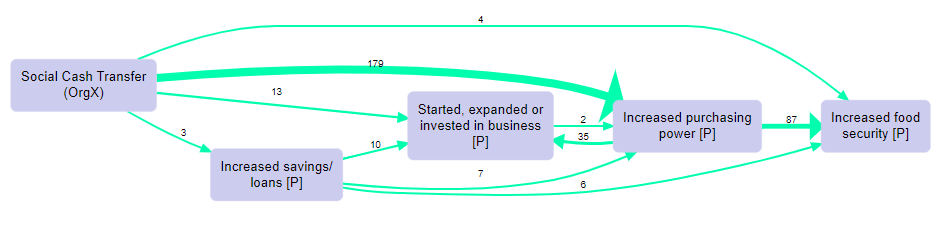
\includegraphics[width=6.77083in,height=\textheight]{_assets/simplify.png}
\caption{img}
\end{figure}

This Guide is for you if:

\begin{itemize}
\tightlist
\item
  you want to find out more about causal mapping as an approach (look for this symbol 📚)
\item
  you want to find out more about the \href{https://causalmap.app/}{Causal Map app} (look for this symbol 💻)
\item
  you are on, or have completed, the \href{https://bathsdr.org/about-the-quip/}{QuIP} Lead Evaluator training
\end{itemize}

\begin{center}\rule{0.5\linewidth}{0.5pt}\end{center}

If you are in a hurry (and who isn't?), look for overview sections and subsections marked with a ⚡.

This Guide accompanies Causal Map 2, the new version of Causal Map, and is valid from September 2021.

The \href{http://guide2.causalmap.app.s3-website.eu-west-2.amazonaws.com/}{old version of this Guide} covers the old version of Causal Map (the one hosted at go.causalmap.app).

\hypertarget{formatting-in-this-guide}{%
\section{Formatting in this guide\ldots{}}\label{formatting-in-this-guide}}

We display statements and quotes from them, respondents' actual words, in quote marks:

``Thanks to the financial support, I can now go to school''

We display factor labels with underlines, like this:

Able to go to school

When we display whole coded causal claims which include an arrow, we don't use the underlines:

Financial support ➜ Able to go to school

This first part of the Guide covers all the basic ideas of causal mapping. The second part covers some additional ideas, which correspond to the features enabled for those with ``Extra'' subscriptions to the Causal Map app.

\hypertarget{videos}{%
\section{Videos}\label{videos}}

Check out our small but growing library of \href{https://causalmap.app/course/causal-map-basics/}{short, focussed training videos}.

\hypertarget{license}{%
\section*{License}\label{license}}
\addcontentsline{toc}{section}{License}

This guide is licensed to you under \href{http://creativecommons.org/licenses/by-nc-nd/4.0/}{Creative Commons Attribution-NonCommercial-NoDerivatives 4.0 International License}.

\hypertarget{part-introduction}{%
\part{Introduction}\label{part-introduction}}

\hypertarget{x5}{%
\chapter{⚡ Your first 5 minutes with Causal Map}\label{x5}}

The rest of this \href{guide.causalmap.app}{Guide} will take you on a 🗺 \protect\hyperlink{quick-tour}{quick tour} of the app.

When you first login, you will be able to see a number of files in the dropdown list on the left-hand side.

\begin{figure}
\centering
\includegraphics[width=6.77083in,height=\textheight]{_assets/ZwspZWog6A.gif}
\caption{ZwspZWog6A}
\end{figure}

Some of these are standard template files everyone can see - so if you have simply been asked to log in to view a whole project, make sure you know the file name that you should be looking at. Alternatively, you may have been \protect\hyperlink{xinvite}{sent a link} to a specific filtered map.

Once you load a file you can see how data has been \protect\hyperlink{xcoding-panel}{coded}, look at transcripts using the \protect\hyperlink{xstatement-nav}{`book' buttons}, or create your own maps using the \href{xintro-filters}{filters}. Example 2 is a good place to start, it is the default file and so will already be loaded. You won't be able to change anything as you will have View Only access, but \protect\hyperlink{quick-tour}{take a look around} and have a play with the \protect\hyperlink{xintro-filters}{filters} and \href{x\#all-tables}{tables}.

If you want to try out some coding yourself, why not \protect\hyperlink{xown-copy}{copy an example file} and with the help of the \protect\hyperlink{xcoding-panel}{coding section} of this guide give it a go?

\hypertarget{xinvite}{%
\chapter{Just received an invite to view something in Causal Map?}\label{xinvite}}

Someone sent you a link like \url{https://causalmap.shinyapps.io/CausalMap2/?s=99} so you can view and explore their file?

Assuming they also remembered to give you permissions to view the file :smile: once you are logged in, the link will take you straight to a specific view of a specific file (a specific map or table) with a specific set of filters applied. You can then add or take away your own filters if you would like to explore further.

\hypertarget{moving-to-causal-map-2-from-causal-map-1}{%
\chapter{Moving to Causal Map 2 from Causal Map 1}\label{moving-to-causal-map-2-from-causal-map-1}}

\textbf{Read this if you have been using the legacy version of Causal Map (CM1) at go.causalmap.app}

All your files (and other files you had access to) from CM1 are accessible from within CM2. You will find them in the file chooser dropdown menu as before, but preceded by \texttt{cm1/...}

\begin{figure}
\centering
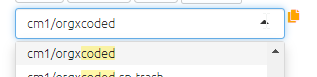
\includegraphics[width=6.77083in,height=\textheight]{_assets/image-20210914103154772.png}
\caption{image-20210914103154772}
\end{figure}

You can view and analyse these files in CM2 without needing to do anything.

You can't make changes to them from within CM2.

If you are still coding a file in CM1, changes you make will be visible from CM2 as soon as you refresh the page.

If you want, you can save a CM1 file in the new CM2 format so that you can continue to edit it in CM2 (as long as you have \emph{edit} or c\emph{opy}, not just \emph{view}, authorisation to the original file- see \protect\hyperlink{xpermissions}{here} for more details).

\begin{figure}
\centering

\includegraphics[width=6.77083in,height=\textheight]{_assets/image-20210921103613356.png}
\caption{image-20210921103613356}
\end{figure}

This creates a new file which is no longer connected to the original file.

You will find that \emph{coding} with the new platform is pretty much the same as coding in the old one. The Factor Editor aka multi-editor is still there but on the right hand side. But when it comes to \emph{analysis}, the new app can do much more.

The rest of this \href{guide.causalmap.app}{Guide} will take you on a 🗺 \protect\hyperlink{quick-tour}{quick tour} of the app.

You may also have been using the Causal Map \textbf{Viewer} at (\url{https://causalmap.shinyapps.io/CausalMapViewer/}). This has been superseded by Causal Map 2.

\hypertarget{are-causal-map-and-causal-mapping-for-me}{%
\chapter{📚 Are Causal Map and causal mapping for me?}\label{are-causal-map-and-causal-mapping-for-me}}

So, you've taken a look at the \textbf{\href{https://causalmap.app/the-app/}{features of the app}}, and you're getting excited about creating maps -- but is your project right for it?

Use Causal Map if you:

\begin{itemize}
\tightlist
\item
  have a relatively large amount of narrative data (enough to provide at least 20-30 causal links)
\item
  need help to organise a large number of links and summarise them into an overview or synthesis
\item
  have information from more than one source (for example different respondents, different documents, or different places in one document) and the information about the source is important to you: they aren't all interchangeable
\item
  are interested in possible differences between the sources and groups of sources -- and/or you don't necessarily have a preconceived idea of the contents or boundaries of the map.
\item
  want to capture what your sources actually say, systematically and transparently
\end{itemize}

Causal Map map is not suitable if you:

\begin{itemize}
\tightlist
\item
  only have a relatively small map which you can manage with traditional tools for drawing network diagrams (e.g.~PowerPoint, \href{http://kumu.io}{kumu.io} etc.)
\item
  need to analyse quantitative data and/or need to do precise mathematical modelling, e.g.~of future states of a system under certain conditions
\item
  would like to sketch out a plan (e.g.~Theory of Change or similar) without much reference to the different sources underpinning each link
\end{itemize}

\hypertarget{features-of-causal-map}{%
\chapter{Features of Causal Map}\label{features-of-causal-map}}

\hypertarget{main-features-of-causal-map}{%
\section{Main features of Causal Map}\label{main-features-of-causal-map}}

\begin{itemize}
\tightlist
\item
  Code causal claims in the form A --\textgreater{} B
\item
  Code multiple claims at once
\item
  Code additional claims as a continuation of previous claim (``\protect\hyperlink{xchaining-links}{chaining}'')
\item
  \protect\hyperlink{ximport}{Import data} (and meta-data about your sources) in different formats
\item
  Add \protect\hyperlink{xmemosandhashtags}{memos and hashtags}
\item
  See a summary of all statements from a specific source
\item
  View additional information about each statement (e.g.~question and respondent characteristics)
\item
  Create simple or \protect\hyperlink{xhierarchical-coding}{hierarchical factor labels}
\item
  Edit many factors and links at once in a \protect\hyperlink{factor-editor}{powerful bulk editor}
\item
  Filter the global map by: Current statement; Factor label; Link (quote, hashtag, memo etc); Statement (text, additional data e.g.~respondent characteristics)
\item
  \protect\hyperlink{xrobustness}{Trace paths} from one set of factors to another
\item
  Use the interactive viewer to edit your map
\item
  View and export print-quality maps
\item
  View all quotes for a specific view, and get a smart summary
\item
  Create detailed \protect\hyperlink{core-tables}{tables}: Factors; Sample; Questions; Closed questions
\item
  Calculate \protect\hyperlink{xrobustness}{\textbf{Robustness of Argument}} for causal paths between sets of factors
\item
  \protect\hyperlink{xroundtripping}{Download/export} your data in different formats
\item
  Share files with others for viewing or editing
\item
  Code additional properties of links like strength and certainty, or mark pairs of factors which are opposite to one another
\end{itemize}

\hypertarget{additional-new-features-in-causal-map-2}{%
\section{Additional new features in Causal Map 2}\label{additional-new-features-in-causal-map-2}}

\begin{itemize}
\item
  Anyone can use it, and it is free for small projects
\item
  Conditional formatting makes your findings more visible
\item
  \protect\hyperlink{xbundlefactors}{Bundle factors} together to make your map neater and easier to read
\item
  \protect\hyperlink{bundlelinks}{Bundle links} by attributes such as stakeholder, district, question and many more
\item
  Infinite versioning means you can restore any change made to a file from any timepoint. This isn't just backups, it is every single change
\item
  It is easier to import and manage your data
\item
  You can import a standard-format Excel file into CM2, meaning you can download a file, edit it, and upload it again (this is called ``\protect\hyperlink{xroundtripping}{round-tripping}''). You can also include any additional fields or columns you want and they will be imported and available for searching, conditional formatting etc
\item
  Build a map by importing any combination of tables or just some of them - factors, links, sources, questions and statements, in any order, at any time
\item
  All outputs transparently recreatable from the \protect\hyperlink{advanced-editor}{filters}
\item
  Share or save links to maps and filters
\item
  Clickable legends and ordinary-language explanations of filters
\item
  Merging maps means you can compare multiple maps:

  \begin{itemize}
  \tightlist
  \item
    You can use the merge\_map filter to temporarily merge other files into the current file if you wish. You can share a link to that merge and revisit it. Viewing a merge of file A and file B will take longer, so you will probably want to save the merged file as a new file
  \item
    The tables (factors, links etc) have a new field called factor\_map\_id etc, which you can use to visualise the merge e.g.~by presenting links in a different colour according to their source
  \end{itemize}
\item
  You can restore, lock, delete, archive and share any of your files
\item
  Log in to the same or different maps from the same or different accounts, including from multiple browser tabs
\item
  Collaborate on a file asynchronously
\item
  View, filter and sort all the tables - factors, links, sources, questions and statements - making up a map. These tables provide all the existing tables functionality plus more.
\item
  Delete factors and edit or delete links directly from the interactive map
\item
  Create a new blank file
\item
  \protect\hyperlink{xown-copy}{Clone an existing file} under a new name, containing all the current factors or only including the factors currently visible
\item
  New colour scales are colour-blind friendly and make sense when printed in black and white
\item
  Like Print View, if Interactive View is given a very big map with lots of links, it now bundles up the links so that it loads faster (you can still view a random quote from the bundle when you hover over a link)
\item
  When you edit a link, you are able to replace it with more than one link if you wish, e.g.~you can edit a link A→B and replace it with A→B and A→C by typing both B and C in the consequence factor box.
\end{itemize}

\hypertarget{glossary}{%
\chapter{⚡ 📚 Glossary}\label{glossary}}

\hypertarget{generic-terminology-for-causal-mapping}{%
\section{Generic terminology for causal mapping}\label{generic-terminology-for-causal-mapping}}

\begin{longtable}[]{@{}
  >{\raggedright\arraybackslash}p{(\columnwidth - 2\tabcolsep) * \real{0.15}}
  >{\raggedright\arraybackslash}p{(\columnwidth - 2\tabcolsep) * \real{0.85}}@{}}
\toprule
\begin{minipage}[b]{\linewidth}\raggedright
Term
\end{minipage} & \begin{minipage}[b]{\linewidth}\raggedright
\textbf{Definition}
\end{minipage} \\
\midrule
\endhead
\textbf{Active filter bar} & This is the first white bar in the filters panel, if your filter is there it is active. \\
\textbf{All filter bar} & This is the second white bar in the filters panel, if your filter is there it is not active, or it is active but can also be used again. \\
\textbf{Bundle} & You can bundle links or factors. Bundling factors merges factors containing a chosen word or phrase. You can also bundle links which are between the same influence and consequence factors, which are usually mentioned in different statements by different sources. A thicker line or a label can be used to show the number of links in the bundle. \\
\textbf{Causal links} & Causal links are the links between the consequence and influence factors. Each link represents a casual claim. \\
\textbf{Combining opposites} & When we combine any pairs of factors which are opposites. This means merging two factors which are identical apart from one starts with a `\textasciitilde{}', to indicate a negative. On print view the link will show green and pink to indicate that both the positive and negative of the factor is true. \\
\textbf{Consequence factor} & A causal factor at the end of a link, that has been influenced by another factor. \\
\textbf{Field} & Additional data associated with a statement such as respondent ID number, respondent age or question number. \\
\textbf{Flags} aka themes & A recurring subject found within the factor labels i.e.~farming or health. Often we use symbols like \# to make sure that the flags are uniquely searchable. \\
\textbf{Hierarchical coding} & Nested factors (see below) put factor labels in a hierarchy from more general to specific. \protect\hyperlink{simplifying}{See more here.} \\
\textbf{Hybrid format} & (Mostly used in QuIP/BSDR coding.) When importing data into Causal Map, a data table in hybrid format has some rows which are statements and some which are metadata. \\
\textbf{Influence factor} & A causal factor at the beginning of the link, that affects another factor. \\
\textbf{Mapfile}, \textbf{File} & When working in Causal Map, all your original data (the statements, source and question data) as well as the coding you have done (factors and links) are stored together in one file which we call a \textbf{mapfile}, or just \textbf{file}. \\
\textbf{Memos} & You can make short notes or memos on each statement, as well as about each causal link, each factor, each source, each question and the project globally. \\
\textbf{Nested factors} & Factor labels can be nested meaning there are higher level factors i.e New intervention; midwife training; hand washing instructions. \protect\hyperlink{simplifying}{See more here.} \\
\textbf{Original links} & Often, there is more than one link between any pair of factors. We can call these the original links especially when we bundle them together for display purposes so they visually look like one. In this case we can say that the bundled link on the map actually consists of several original links. \\
\textbf{Shortlink} & A weblink (URL) to a causal map which has been shortened, usually to make sharing it easier. You can easily make \protect\hyperlink{xshortlinks}{shortlinks} using a button in the app. \\
\textbf{Statement} & Refers to each individual piece of text to be coded in Causal Map, usually this is a sentence, a paragraph or a few paragraphs. Each statement has an ID; a number like 1, 2, 3 etc. \\
\textbf{Source} & Sources are where your statements come from, this could be respondents you have interviewed or documents you have collected. \\
\textbf{Weblink} & A complete URL like \url{https://causalmap.shinyapps.io/CausalMap2/} \\
\bottomrule
\end{longtable}

\hypertarget{part-getting-started}{%
\part{💻 Getting Started}\label{part-getting-started}}

\hypertarget{prerequisites-for-using-the-app}{%
\chapter{⚡ Prerequisites for using the app}\label{prerequisites-for-using-the-app}}

The app is tested on Chrome and Firefox on Mac and Windows, and Safari on Mac, and the new Edge on Windows, and it should work fine on Chrome, Chromium and Firefox on Linux.

You need a screen with a large resolution, preferably HD or better. It won't work well on tablet or phone. You will probably want to zoom out to about 90\% (in Chrome, press Ctrl -- once or twice) to make sure everything fits on the screen. You may also like to view the app ``full screen'' -- how to do this depends on your browser and operating system; on Chrome on Windows, press F11.

As Causal Map is a web application, you will also need a reasonably reliable internet connection.

\hypertarget{signing-up-and-signing-in-at-causal-map}{%
\chapter{⚡ Signing up and signing in at Causal Map}\label{signing-up-and-signing-in-at-causal-map}}

Start your journey at \url{https://causalmap.shinyapps.io/CausalMap2/}.

You can sign in with a Google account.

If you have a paid subscription, however you sign in, make sure the associated email is the same as the one for which you have a subscription. There are a variety of options when it comes to subscriptions, so have a \href{https://causalmap.app/subscriptions/}{look} and find the one that is right for you.

If someone has \protect\hyperlink{xpermissions}{shared files} with you, however you sign in, make sure the associated email is the one the files were shared to.

\hypertarget{collaborating-at-causal-map}{%
\chapter{Collaborating at Causal Map}\label{collaborating-at-causal-map}}

\hypertarget{collaboration}{%
\section{Collaboration}\label{collaboration}}

At the moment, you can log in to the same or different maps from the same or different accounts, including from multiple browser tabs -- so you can have two maps open at once.

Two different people \emph{can} edit the same file. However at the moment the results can be unpredictable and we recommend working asynchronously (taking it in turns.) If you are viewing a file while someone else edits it, you will have to refresh to see any changes they made.

\hypertarget{teams}{%
\section{Teams}\label{teams}}

\begin{figure}
\centering
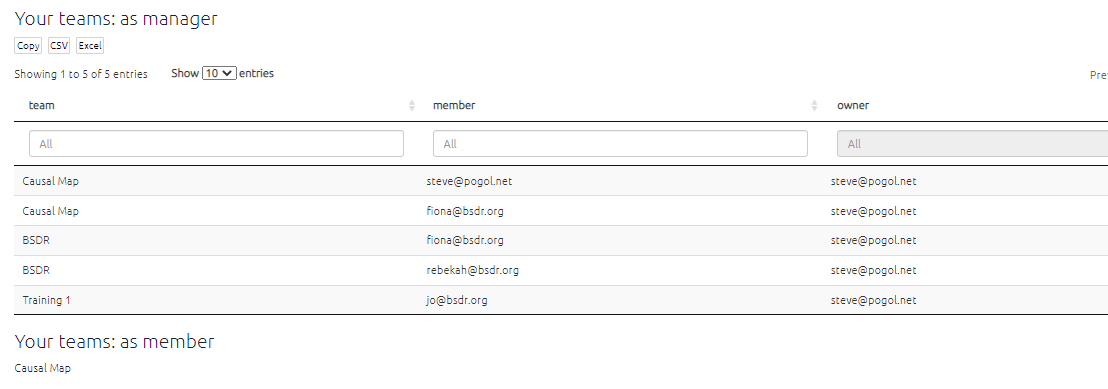
\includegraphics{_assets/image-20211106103853413.png}
\caption{image-20211106103853413}
\end{figure}

\begin{itemize}
\tightlist
\item
  You can create one or more teams and make other people members of that team
\item
  Other people can include you in their teams
\item
  Each team has an owner and a name, and one or more members
\item
  The names of teams you are a member of appear in sha
\item
  There is a special team called \texttt{global}: sharing a file with \texttt{global} means that any user of Causal Map gets access.
\end{itemize}

\hypertarget{quick-tour}{%
\chapter{⚡ Quick tour of the app}\label{quick-tour}}

The app has two parts, the \protect\hyperlink{xlhs}{left-hand side} and the \protect\hyperlink{rhs}{right-hand side}.

You can get help at any time by clicking on the little blue info buttons, like below. This will then open a panel displaying the relevant section of this guide.

\begin{figure}
\centering

\includegraphics{_assets/image-20210927115203506.png}
\caption{image-20210927115203506}
\end{figure}

\hypertarget{xlhs}{%
\section{The left-hand side}\label{xlhs}}

\hypertarget{getting-data-into-the-app}{%
\subsection{Getting data into the app}\label{getting-data-into-the-app}}

\begin{itemize}
\tightlist
\item
  Upload a map in the form of an \protect\hyperlink{xuploading-and-updating}{Excel file} (.xls or .xlsx).
\item
  In the file chooser, select any files to which you have access, which include an anonymised dataset from a \href{http://bathsdr.org/}{QuIP} study.
\item
  Follow a direct link sent to you by someone else to view a file with pre-defined filters applied and which you can then explore for yourself.
\item
  view maps created in the \href{http://causalmap.app/}{legacy version of Causal Map}.
\end{itemize}

\hypertarget{commands-and-buttons-to-apply-filters-to-your-map}{%
\subsection{Commands and buttons to apply filters to your map}\label{commands-and-buttons-to-apply-filters-to-your-map}}

The left-hand side of the app really only contains the text in the Advanced Editor (which you can view if you want, but close the window if it scares you).

\begin{figure}
\centering
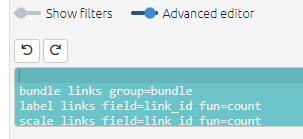
\includegraphics{_assets/image-20210914103354673.png}
\caption{advanced-editor}
\end{figure}

The text window uses a simple syntax for filtering and manipulating the maps and tables.

Nearly all the other buttons on the left-hand side are just ways to manipulate this text. Each line in this window is a filter which manipulates the existing map in some way. The lines in the windows are applied successively to the original map to produce the final map which is then displayed.

\hypertarget{xstatement-view}{%
\subsection{Do some coding (view one statement) or do some analysis (view many statements)?}\label{xstatement-view}}

\begin{figure}
\centering

\includegraphics{_assets/image-20211026110623336.png}
\caption{\#statement-toggle}
\end{figure}

These buttons add the correct filters to either view just one statement or many statements.

When you are coding, you will want to view just one statement, and when you want to explore and analyse the entire causal map or sections of it, you will want to view many statements.

(Even when you are viewing one statement, it is still possible to apply filters for example if the map associated with this one statement is quite large.)

\hypertarget{top-row}{%
\subsection{Top row}\label{top-row}}

Most people like to hide these filters when they are coding, so they hide the filters using the toggle.

\begin{figure}
\centering

\includegraphics{_assets/image-20210914103505559.png}
\caption{image-20210914103505559}
\end{figure}

But for analysing your map, you will want to open the filters panel.

\hypertarget{shortcut-buttons}{%
\subsection{Shortcut buttons}\label{shortcut-buttons}}

These buttons offer quick ways to add filters without going through a dialog panel.

\hypertarget{the-filter-buttons}{%
\subsection{The filter buttons}\label{the-filter-buttons}}

There are in three sections: analysis, conditional formats and simple formats. See the section on \href{https://guide.causalmap.app/all-the-filters.html}{filters}.

\hypertarget{xadditional-informati}{%
\subsection{Additional Information}\label{xadditional-informati}}

To see additional information about the statement you are currently viewing such as the \texttt{source\_id} and \texttt{question\_id} slide the info toggle.
\includegraphics{_assets/image-20211220153438354.png}

\hypertarget{rhs}{%
\section{The right hand side}\label{rhs}}

\begin{figure}
\centering

\includegraphics[width=6.77083in,height=\textheight]{_assets/image-20210914103654314.png}
\caption{image-20210914103654314}
\end{figure}

\hypertarget{not2}{%
\subsection{Interactive View}\label{not2}}

An interactive version of the map in which the elements can be moved around and also the upstream and downstream factors are highlighted when the user moves their mouse over them.

\hypertarget{not}{%
\subsection{Print View}\label{not}}

A print-quality version of the map with advanced layout.

\hypertarget{no-not-this-one}{%
\subsection{Factor editor}\label{no-not-this-one}}

Simply click on the factor you want to change and edit it. You can change one factor everywhere in the file or you can do it for each statement, by pressing the Split checkbox. Just remember to press update once you have made your changes and you are happy with them.

\hypertarget{tables}{%
\subsection{Tables}\label{tables}}

Several tables showing lists of factors, links and various metrics and which can be filtered and reorganised in marvellous ways. See the section on \href{https://guide.causalmap.app/all-the-tables.html}{tables}.

\hypertarget{FAQs}{%
\chapter{⚡ FAQs: Causal Map questions and troubleshooting}\label{FAQs}}

\hypertarget{logging-in}{%
\section{Logging in}\label{logging-in}}

There seems to be a problem with my current file and every time I refresh the page the app kicks me out again

Most likely there is a problem with your current file. Refresh the page, and click the button here as soon as it reloads.

\includegraphics{_assets/image-20211117201957585.png}
Wait a little to return to the main screen. Then try to load your file. If you still can't load it, use the blue feedback button on the far right to report the issue to our support team.

I can't log in

If you have the app open in more than one browser tab, close all those tabs and load the app again. If you still can't load it, contact our support team.

\hypertarget{setting-up}{%
\section{Setting Up}\label{setting-up}}

Is there a security audit for Causal Map?

Please see our T\&Cs at \url{https://causalmap.app/terms-and-conditions-for-the-causal-map-app/}

I've signed up but haven't received a validation code?

Firstly, the best thing to do is double check you have entered your email correctly - if your email is correct, then try sending the code again. Make sure to also check your junk/spam email folder. If none of these things work email us at \href{mailto:hello@causalmap}{\nolinkurl{hello@causalmap}}.

How do I import and export maps from Causal Map 2?

You can download your map from Causal Map 2 as an Excel file, tweak it and then upload it Causal Map 2.

I have done something wrong, how do I know which version to restore?

Have a look in the Updates tab. You can't actually restore the file from here but you can maybe guess which one you want by looking at the number of factors, the last coded statement etc.
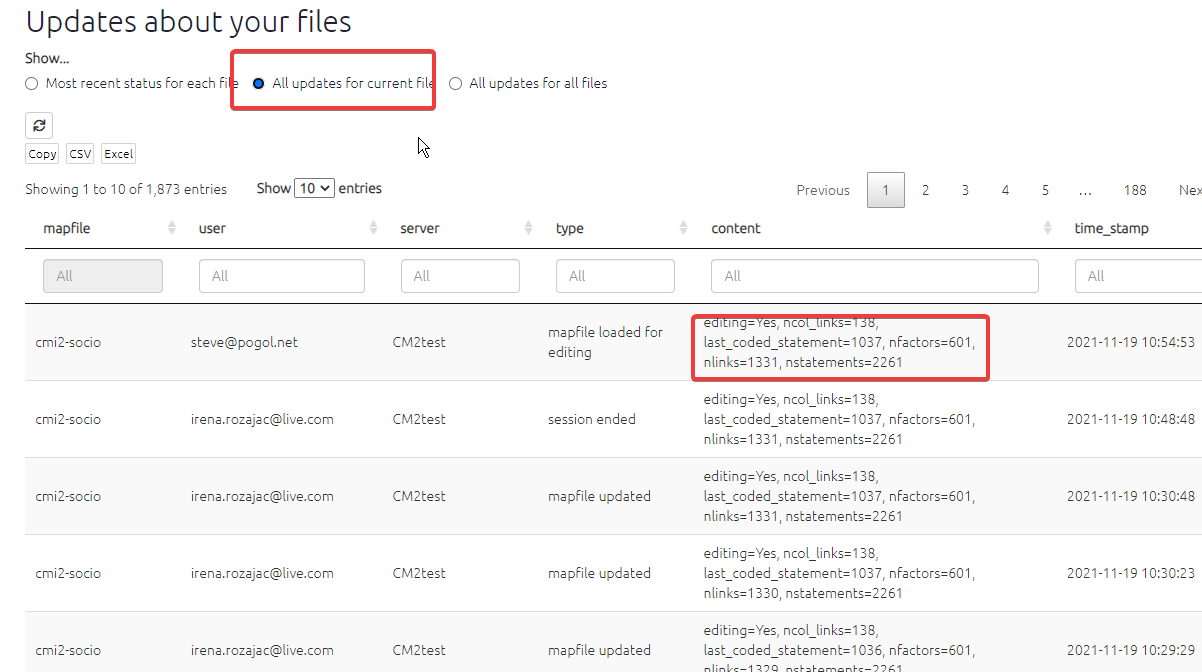
\includegraphics{_assets/image-20211119105900995.png}

I made changes to file access with the Files panel, but they aren't working

Refresh the browser and your changes should appear.

Can I upload data with special characters in e.g.~à, è, ù, б, ж ?

Yes, the app will import them.

\hypertarget{uploading-and-tweaking-data}{%
\section{Uploading and tweaking data}\label{uploading-and-tweaking-data}}

When I upload new or updated data into the app, does it matter what the spreadsheet file is called?

No.~The only thing that matters is what file you are uploading \emph{into} at Causal Map: the currently active file.

\hypertarget{coding}{%
\section{Coding}\label{coding}}

When I highlight a single word or very short phrase, why is the same word highlighted but in a different part of the statement?

If you highlight a very short piece of text which happens to appear (exactly the same) more than once in the statement, it is always the first occurrence of this piece of text which is actually highlighted.

I have some factors with no links at all, how can I get rid of them?

Sometimes you might want to keep these factors because they are part of a fixed codebook. But it you don't want them, go to the Data tab and click the link to delete them.

The quote doesn't match up with the statement number?

If you are looking at statement 99, looking also at factor editor, and click a quote to edit that link, which is actually say link 66 from statement 11, then the text from statement 11 will load up and link 66 will load up but the statement navigator above still says 99. That isn't wrong, it is just confusing! The filter you originally set to look at statement 99 hasn't changed.

Can I edit more than one link at a time?

No, currently you can only edit one link at a time.

Can I autofill influence factor label if its the same as the last consequence factor?

Yes, that is called chaining links! You can chain links by clicking the chain icon, after you have saved your previous link. If you would like more guidance check out this video.

I'm all zoomed out, how do I get a normal zoom level in my browser?

If you have Windows press ctrl and 0. If you have a Mac press option, command and 0.

Can I create more than one link at a time?

Yes. You can create multiple links at a time just by putting more than one factor in either or both boxes.If you want more information check out this short video.

How do I link two existing chains?

To link a chain a --\textgreater{} b --\textgreater{} c to a chain d --\textgreater{} e, highlight the part of the statement which provides the evidence and then code a link from c to d using the dropdowns as usual.

If a respondent makes the same causal claim twice, should I code it twice?

If they are just repeating the same point, don't bother. But if they are bringing different evidence for the same link, code it twice.

Should I put spaces after \texttt{;} in hierarchical coding? What about after \texttt{\textasciitilde{}} when coding opposites?

The convention is this: blah; blah

blah; \textasciitilde blah

etc, i.e.~we put a space after the ; but no space after the \textasciitilde{}

Can I trace paths from one factor to ``everything''?

No, because it doesn't really make sense \ldots. would you want to trace the paths to every single factor in the map? Or if not, which ones? (It would maybe make sense to ask about the impact of ``something'' on \emph{all the endpoints which have no more children}, but we are not sure how useful it would be.) What you'd have to do is say flag all the factors you are interested in (say by adding the flag ``!Outcome'') and then trace the paths from some input factor(s) to all of these, which you can easily do just by typing ``!Outcome'' in the box.

What do \texttt{unique} and \texttt{literal} mean?

You use \texttt{unique} and \texttt{literal} when you don't want to do any counting, you want to print or otherwise use the actual values. So if you have a bundle with sources a, a, b and c, and you want to print them as labels, then unique: source\_id will print a; b; c whereas litera: source\_id will print literally a; a; b; c

\hypertarget{known-bugs}{%
\section{Known Bugs}\label{known-bugs}}

When I highlight text which overlaps with a previously highlighted section no new highlight appears.

Unfortunately there is no easy fix for this bug but it is just cosmetic. You can check you have highlighted the right section by checking the text box below the factor label boxes contains the text you want to highlight. Once you have saved the link the highlight will appear on the statement.

When I use literal labels on my links e.g.~to list all the sources like ``AM1; AM3; AM5'', I can't use \texttt{wrap\ links} to wrap the link labels and insert line breaks, I just get some very long labels.

This is just the way the Causal Map functions work, we will fix it sometime, sorry.

\hypertarget{quip-questions}{%
\section{QuIP questions}\label{quip-questions}}

How do I import my QuIP project into Causal Map?

You must create an excel file with four columns. The column headers must be in this order; text/answers, source\_id, question\_code and question\_text. Then upload this to a blank file using the purple upload button for hybrid files. For more information see this section

\hypertarget{downloads}{%
\section{Downloads}\label{downloads}}

Example files, which can be used as templates, can be found and downloaded \href{https://drive.google.com/drive/folders/1wvifDQ0BXmAjSudTRUv9i_4JURpphD4v}{here}.

\hypertarget{part-the-app-panel-by-panel}{%
\part{💻 The app, panel by panel}\label{part-the-app-panel-by-panel}}

\hypertarget{xtop-menu}{%
\chapter{⚡ The top menu}\label{xtop-menu}}

This section is all about how to manage using the top menu to help you deal with the currently loaded file. Hover over the icons to see what they do.

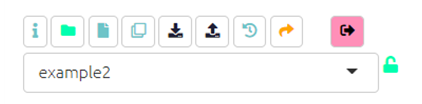
\includegraphics[width=6.77083in,height=\textheight]{_assets/image-20211025111815970.png}

You can use these buttons for quick fixes. There is also a dedicated \protect\hyperlink{file-manager}{File Manager} to manage all your files.

\hypertarget{xpermissions}{%
\section{Current File Manager}\label{xpermissions}}

Click the green File icon to manage your file.

\begin{figure}
\centering
\includegraphics[width=6.77083in,height=\textheight]{_assets/uBfaYOvRRH.gif}
\caption{uBfaYOvRRH}
\end{figure}

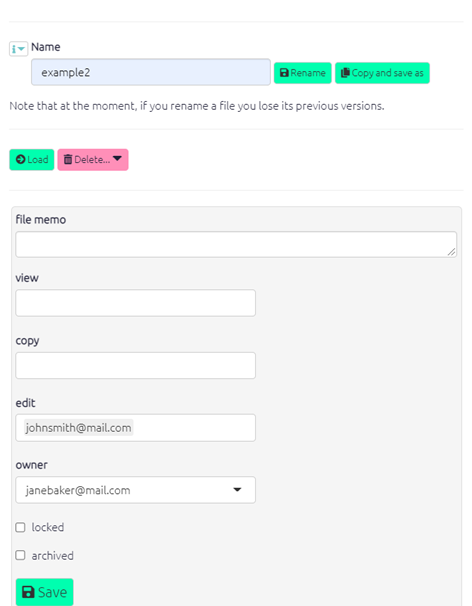
\includegraphics[width=6.77083in,height=\textheight]{_assets/image-20211025111538915.png}

\hypertarget{sharing-and-locking-files}{%
\subsection{Sharing and locking files}\label{sharing-and-locking-files}}

You can add any number of other Causal Map accounts into the ``copy'' and/or ``view'' boxes.

\begin{itemize}
\item
  ``Copy'' permission means that the other user can make their own copy of this file, which they can then edit.
\item
  ``View'' permission means that the other user can make only view the file.
\end{itemize}

You can also use this switch to lock the file. This means that no-one can change it, not even you, until it is unlocked again.

It is also possible to create larger groups of users. Ask us for help with this: \href{mailto:hello@causalmap.app}{\nolinkurl{hello@causalmap.app}}.

\hypertarget{file-memo}{%
\subsection{File memo}\label{file-memo}}

You can put information about your file in the \texttt{file\ memo} box, and it will be shown below the interactive map to tell other users what this file is about. You can use markdown to format the text, e.g.~start a line with \# to make level-1 heading. You can even include images using markdown.

\begin{figure}
\centering
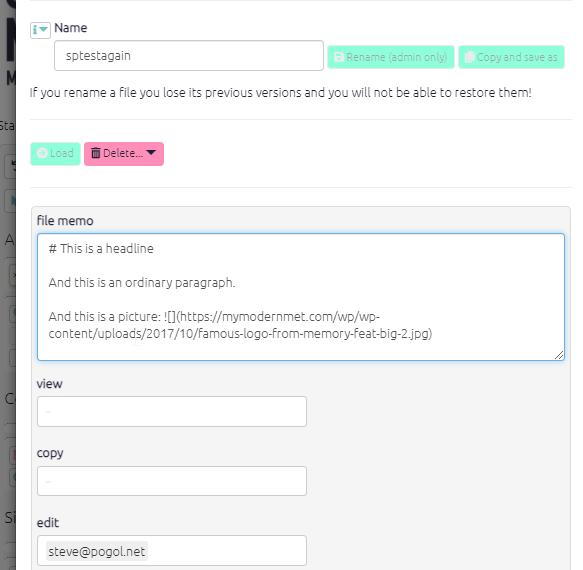
\includegraphics{_assets/image-20211103133030379.png}
\caption{image-20211103133030379}
\end{figure}

This is in addition to any ``newsflash'' information about updates which you add using the chat widget.

\hypertarget{xown-copy}{%
\section{⚡ Making your own copy of a file}\label{xown-copy}}

\href{https://player.vimeo.com/video/641927229}{\includegraphics{Guide-to-causal-mapping_files/figure-latex/unnamed-chunk-1-1.pdf}}
Copying a file in Causal Map is easily done. Simply load the file you want to copy using the dropdown menu. Then click the `Save As' button on the top left of your screen.

\includegraphics[width=6.77083in,height=\textheight]{_assets/5Najfi4Pr2.gif}

You can then append something to the end of the filename to make it yours:

\begin{figure}
\centering
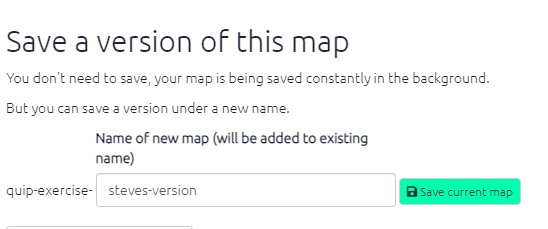
\includegraphics[width=6.77083in,height=\textheight]{_assets/image-20211001180419448.png}
\caption{image-20211001180419448}
\end{figure}

Click the `Save current map' button. This window will then close and your copy of the file will load up. You can now make changes to the file.

\hypertarget{restoring-a-previous-version-of-your-file}{%
\section{Restoring a previous version of your file}\label{restoring-a-previous-version-of-your-file}}

The app is continously saving your work and so you can restore your file to any prevision version, by clicking this icon 
\includegraphics{_assets/image-20211115175030770.png}. This will open the below panel where you can choose which timepoint you wish to revert your map to.

\begin{figure}
\centering
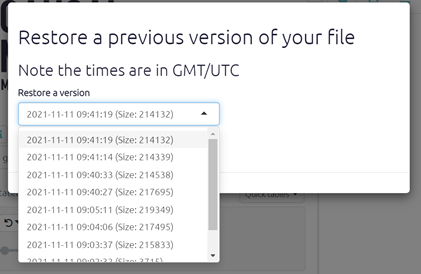
\includegraphics[width=6.77083in,height=\textheight]{_assets/image-20211115174934976.png}
\caption{image-20211115174934976}
\end{figure}

This panel shows a dropdown list of times when you made changes to the mapfile in GMT. Along with the size of your file which can help you identify which timepoint you want to revert to. It can be easy to forget what time you made alterations to your file, so if you're likely to want to restore a previous map it is best to note the time so that you can easily return to it.

\hypertarget{xshortlinks}{%
\section{Sharing a link using shortlinks}\label{xshortlinks}}

To share a link to a file click the orange arrow on the top panel. You can then add a title for this shortlink, to remind you of its content, but this is optional. The short link will be copied to your clipboard and anyone you send this to will be able to see your map with the current filters applied (providing they have the correct \protect\hyperlink{xpermissions}{permissions}).

\begin{figure}
\centering
\includegraphics[width=6.77083in,height=\textheight]{_assets/6vEfSLFOlx.gif}
\caption{6vEfSLFOlx}
\end{figure}

The server which a shortlink takes you to is (obviously?) the one in the shortlink itself. So \url{https://causalmap.shinyapps.io/CM2test/?s=138} takes you to the Test server whereas if you change the server name to \url{https://causalmap.shinyapps.io/CausalMap2?s=138} that will recreate the same filter on the Production server.

Shortlinks also store information about when the link was created.

\hypertarget{uploading-your-data}{%
\section{Uploading your data}\label{uploading-your-data}}

\begin{figure}
\centering

\includegraphics[width=6.77083in,height=\textheight]{_assets/image-20211115175648298.png}
\caption{image-20211115175648298}
\end{figure}

The above buttons relate to uploading your data, see \protect\hyperlink{xuploading-and-updating}{this section} for more information.

\hypertarget{chat-about-this-file}{%
\section{Chat about this file}\label{chat-about-this-file}}

By clicking on the icon of two speech bubbles, a panel containing chat about the file will appear. You can see the comments you and other people with access to this file have added. From here you can also add updates on this file, this function is useful when working collaboratively.

\begin{figure}
\centering
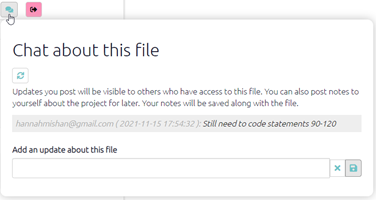
\includegraphics{_assets/image-20211115175519249.png}
\caption{image-20211115175519249}
\end{figure}

\begin{quote}
Why did I make this version of that file? Is it different from version xzy? Did we already import those new statements into this version??
\end{quote}

This panel can help with these kinds of problems. You and your colleagues -- anyone else with access to the current file -- can type notes and updates about the file. These updates will be listed here sequentially.

Also, these same notes and updates are listed in the main Updates panel, along with automatic updates about when files were opened and edited.

\begin{figure}
\centering
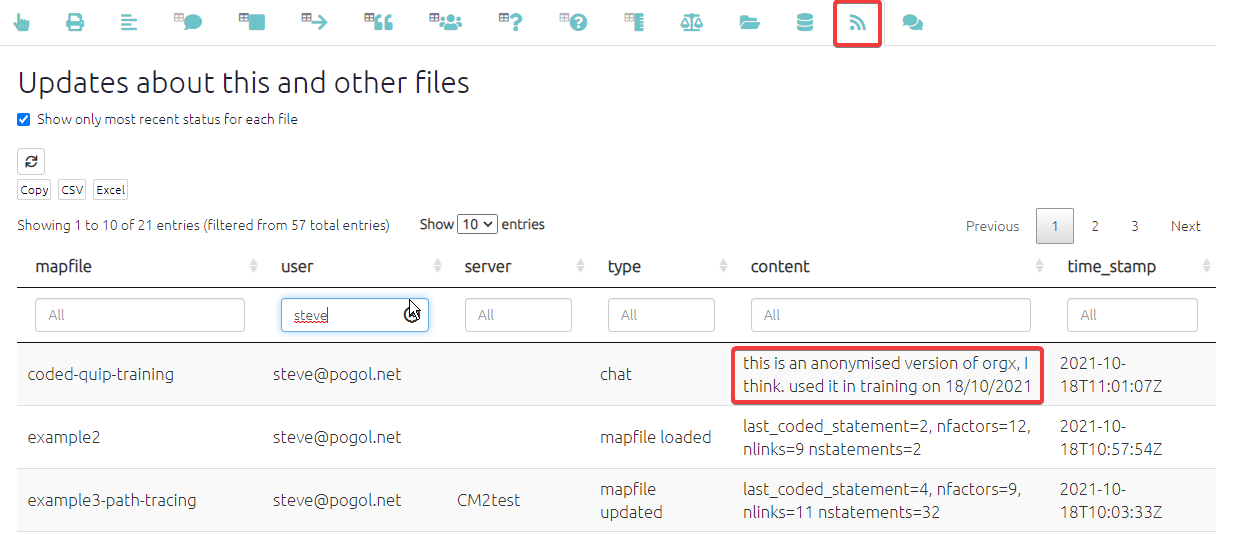
\includegraphics{_assets/image-20211018121359141.png}
\caption{image-20211018121359141}
\end{figure}

So you can use the filters just to search for manual and automatic updates about particular files, or on particular dates; or you can just search for type=chat to view recent chat about any files or some particular files:

\begin{figure}
\centering
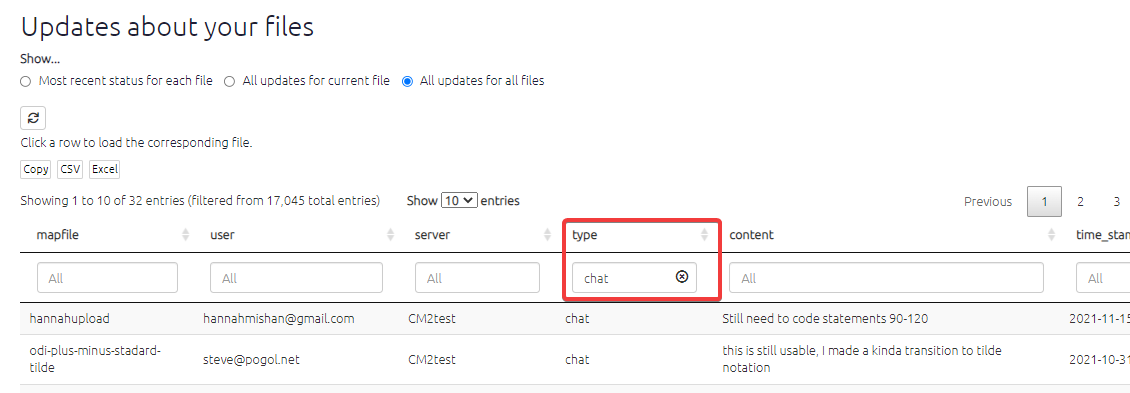
\includegraphics{_assets/image-20211122063223836.png}
\caption{image-20211122063223836}
\end{figure}

\hypertarget{xfile-manager}{%
\chapter{⚡ The File Manager}\label{xfile-manager}}

At the top of the page you will find information about your subscriptions, the files you have crested and any teams you manage.

Below, the file manager table allows you to see shows you all the files you have access to and what level of access you have i.e.~copy, view or edit access. You can also see details such as whether these files are locked, archived, any memos on the file and what access other users have to these files.

\begin{figure}
\centering
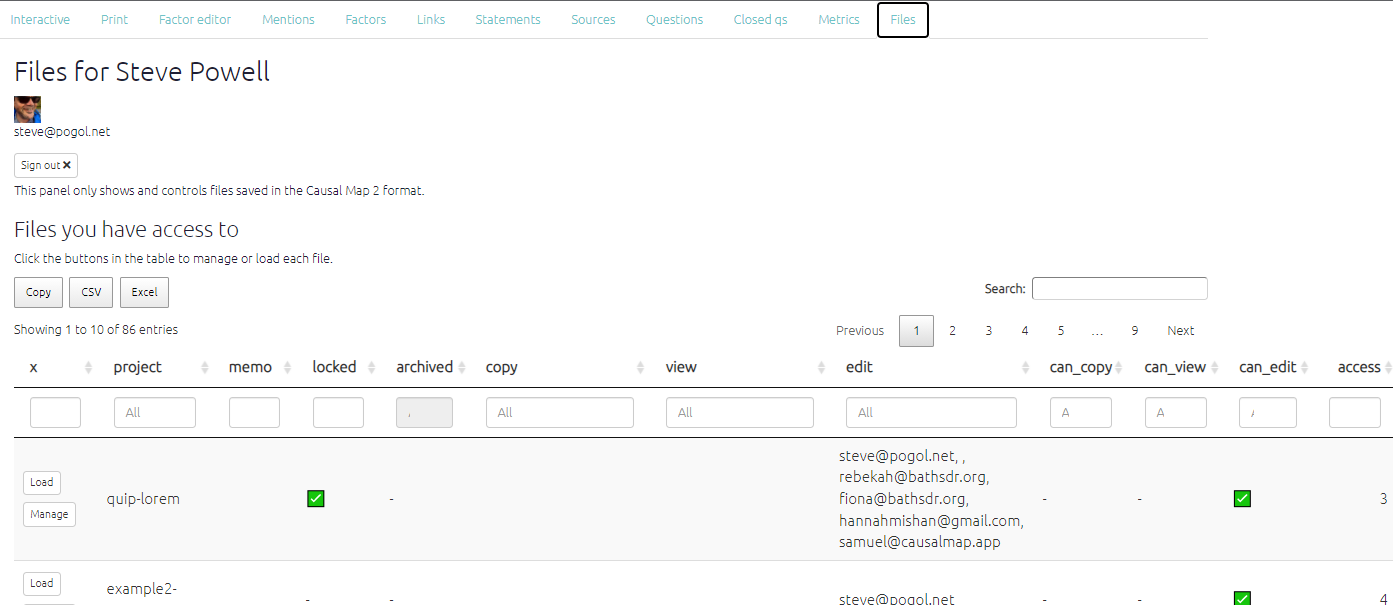
\includegraphics[width=6.77083in,height=\textheight]{_assets/image-20210927120502982.png}
\caption{image-20210927120502982}
\end{figure}

From this page you can either \texttt{load} the map or click \texttt{manage}to open the \protect\hyperlink{xpermissions}{file manager panel}.

\hypertarget{xstatement-nav}{%
\chapter{⚡ The Statement Navigator}\label{xstatement-nav}}

When you are looking at one statement at a time, you will see the navigation bar displayed below.

\begin{figure}
\centering

\includegraphics{_assets/image-20211105092246054.png}
\caption{image-20211105092246054}
\end{figure}

The \texttt{info} toggle opens additional statement info, i.e.~info for any fields which start with \#, for example you might have a field \#gender in your statements table.

\begin{figure}
\centering
\includegraphics{_assets/sm559T6lUE.gif}
\caption{sm559T6lUE}
\end{figure}

Boxes to edit the statement, question and source memos will also appear. Here you can add useful additional data which can be displayed on your map using the \href{xformatting-links}{label links} or \protect\hyperlink{xlabel-factors}{label factors} filters.

\begin{figure}
\centering
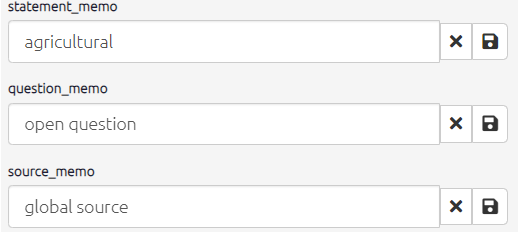
\includegraphics[width=6.77083in,height=\textheight]{_assets/chrome_xXrp2x0TKw.png}
\caption{chrome\_xXrp2x0TKw}
\end{figure}

By clicking on the green book icon you can see all the statements from all sources or the black book icon will show the transcript from the respondent whose statement you are currently viewing.

\begin{figure}
\centering

\includegraphics[width=6.77083in,height=\textheight]{_assets/image-20211108162324112.png}
\caption{image-20211108162324112}
\end{figure}

You can use the arrow and numbered button to skip through statements. If you want to skip to a particular statement the easiest way is to use the \href{xfind-statements-links}{find statements} filter. This will automatically be applied if you are viewing statements one at a time, so simply click on the filter and edit the number it is searching for.

\hypertarget{xcoding-panel}{%
\chapter{⚡ The Coding Panel: creating factors and links}\label{xcoding-panel}}

Qualitative causal mapping involves taking passages of text, e.g.~from interviews or documents, and identifying sections which make causal claims. We highlight each of these sections and specify a causal factor at each end of each link (for example Lost job or Went hungry). This means creating a new factor or reusing an existing one. Usually we create these factors inductively as we code, and revise and review and consolidate them as part of the process, as with any other kind of qualitative content analysis. This section is about how to create factors and their labels.

In Causal Map, a factor \emph{is} its label. Once you create a label, there is nothing else to add.

\hypertarget{creating-links-in-the-app}{%
\section{Creating links in the app}\label{creating-links-in-the-app}}

\href{https://player.vimeo.com/video/588851236}{\includegraphics{Guide-to-causal-mapping_files/figure-latex/unnamed-chunk-2-1.pdf}}

To code a causal link, - With your mouse, highlight a piece of text within the statement which makes a causal claim.

\begin{itemize}
\item
  Watch how that passage is copied for you into the ``Quote'' window below. (Usually you don't need to think about his window: you can edit the text if you really need to but it has to remain an exact quote of one part of the text or you will get a warning.) - Start to type the name of the influence factors at the \textbf{start} of the link(s) which you are going to make, in the first drop-down menu.
\item
  If there is an existing factor which matches what you want, you can select select it.
\item
  Otherwise you will create a new factor with the contents of what you have typed; finish what you have typed with a comma or a tab character if you want to continue to select or create another factor.
\item
  If you want to create more than one link, you can select or create additional factors in the same box.
\item
  When you have finished, press Enter.
\item
  Repeat the process in the other box to specify the factors at the \textbf{end} of the link (or ends of the links).
\item
  Press the green Save button which is now active.
\item
  The link is created in the Map window, colour-coded with the quote which is now highlighted on the left. If you mouse over the highlighted quote, the link in the map is activated.
\end{itemize}

For more information on how to edit an existing link \protect\hyperlink{xedit-factor-and-links}{see here}.

\textbf{NOTE}: factor names which contain semicolons \textbf{;}. get special treatment as they separate the different parts of \emph{hierarchical} labels.

After beginning to create links between factors, one will notice already-coded factors will appear in the dropdown menus in the to and from factor boxes. For added convenience:

\begin{itemize}
\tightlist
\item
  the most frequently coded factors will appear at the top of this list
\item
  if you are using hierarchical coding, top-level components will appear to be selected even if you have not used them explicitly so far. For example, if you have used the factors \texttt{health;\ mental} and \texttt{health;\ physical}, the factor \texttt{health} will appear even if you never used it explicitly. You can then easily create new nested factors such as \texttt{health;\ spiritual}by selecting \texttt{health} and then typing \texttt{;\ spiritual} with a leading ``;''. The app will automatically join these for you into the factor \texttt{health;\ spiritual}.
\item
  once you have selected an influence factor, the order of the choices available for the consequence factor will be silently updated, presenting at the top of the list the most frequently mentioned consequences of the influence factor you have chosen.
\end{itemize}

\hypertarget{xchaining-links}{%
\section{Chaining Links}\label{xchaining-links}}

\href{https://player.vimeo.com/video/588881701}{\includegraphics{Guide-to-causal-mapping_files/figure-latex/unnamed-chunk-3-1.pdf}}

Chaining links is easily done and useful when you have statement where one consequence leads to another, which leads to a third, and so on. To use this function simply click the chain icon below the consequence factor box and the app will automatically fill the influence box with the consequence from your previous link.

\begin{figure}
\centering
\includegraphics[width=6.77083in,height=\textheight]{_assets/md0XWSnpLr.gif}
\caption{md0XWSnpLr}
\end{figure}

\hypertarget{xmemosandhashtags}{%
\section{Using memos and hashtags}\label{xmemosandhashtags}}

\hypertarget{xlink-memos}{%
\subsection{Memos}\label{xlink-memos}}

Qualitative coding usually involves making notes and memos, and you can do this in Causal Map too.

This toggle opens both additional statement info, i.e.~info for any fields which start with \#, for example you might have a field \#gender in your statements table, and also shows the boxes to edit the memos. (In this example, there is no additional information.)

\begin{figure}
\centering
\includegraphics{_assets/esSnHL226V.gif}
\caption{esSnHL226V}
\end{figure}

\hypertarget{xhashtags}{%
\subsection{Hashtags}\label{xhashtags}}

Hashtags are available as a special kind of memo when coding a link: you can use them to provide any kind of additional information, for example:

\begin{itemize}
\tightlist
\item
  where a link is only relevant in a particular context
\item
  where a link is only a hypothesis
\item
  where a link is only projected for the future
\item
  to tag links you want to come back and review
\item
  to add other qualifying information like ``source seems unsure.''
\end{itemize}

As usual in Causal Map, you can apply one or more hashtags, and you can either select existing hashtags or create new ones on the fly.

Later, you can \href{https://guide.causalmap.app/analysis.html\#filtering-the-map-by-link-hashtag-memo}{filter the map} to show only links containing specific hashtags (or parts of hashtags), and also for links which do \emph{not} contain specific hashtags or parts of hashtags.

\hypertarget{interactive-view}{%
\chapter{⚡ Interactive View}\label{interactive-view}}

An interactive version of the map in which the elements can be moved around and also the upstream and downstream factors are highlighted when the user hovers over them.

\begin{itemize}
\tightlist
\item
  Drag the factors around.
\item
  Copy a map as an image by right-clicking on it.
\item
  Save a PNG image by pressing the button at bottom right.
\item
  Hover over factors to highlight the connected links and factors.
\item
  Hover over factors to display basic information about them and delete them from the entire map.
\item
  Hover over links to see the associated quote and other information.
\item
  Click on links to edit or delete them them.
\item
  Click on factors to focus on them.
\end{itemize}

\begin{figure}
\centering
\includegraphics[width=6.77083in,height=\textheight]{_assets/focus.gif}
\caption{image-20211001175928850}
\end{figure}

\begin{itemize}
\tightlist
\item
  Click on factors to edit the label or memo
\end{itemize}

\begin{figure}
\centering
\includegraphics[width=6.77083in,height=\textheight]{_assets/edit.gif}
\caption{image-20211001175928850}
\end{figure}

In both Interactive and Print view, if the factor labels have not been wrapped to any specific width, they are automatically wrapped to 22 characters.

When you have a lot of factors in your map, the selector in the top-right corner of the map can help locate them.

\begin{figure}
\centering
\includegraphics[width=6.77083in,height=\textheight]{_assets/nodeselect.gif}
\caption{image-20211001175928850}
\end{figure}

When you are viewing a single statement, the colour of the links corresponds to the colour of the highlighted sections of text.

\begin{figure}
\centering
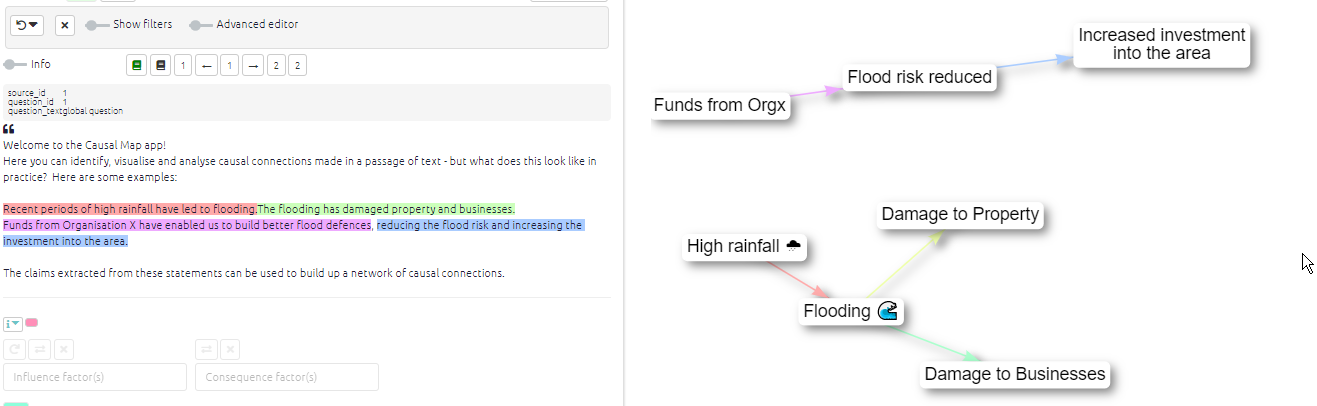
\includegraphics{_assets/image-20211116082854960.png}
\caption{image-20211116082854960}
\end{figure}

\hypertarget{print-view}{%
\chapter{⚡ Print view}\label{print-view}}

A print-quality version of the map with advanced layout. When you are viewing a single statement, the colour of the links corresponds to the colour of the highlighted sections of text.

\begin{itemize}
\item
  If you have edit permissions, you can edit a link by clicking on its label -- if there is no label, click the small dot where the label would be.
\item
  If you have edit permissions, you can edit a factor by clicking on its label.
\item
  If you hover over the link itself (which can be a bit tricky if the link is thin), you will see a tooltip displaying the names of the influence and consequence factors.
\item
  If you hover over the link label you will see a tooltip displaying the link\_ids of the influence and consequence factors.--\textgreater{}
\end{itemize}

\begin{figure}
\centering
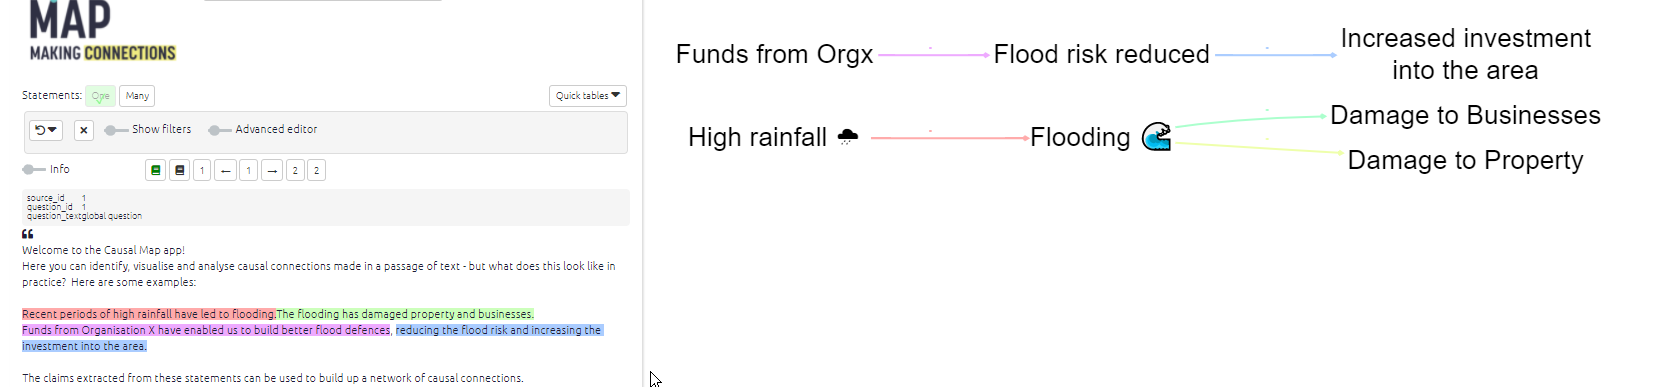
\includegraphics{_assets/image-20211116082645776.png}
\caption{image-20211116082645776}
\end{figure}

To change the format of the print view, use the \protect\hyperlink{xsimple-formats}{set print filter}.

🧪 You can now export your map as SVG using the export SVG button at bottom right.

🧪 You can now, experimentally, change the size of the Print map by double-clicking on it and/or using the \texttt{+} and \texttt{-} buttons. You can also drag it around, which is a bit weird \ldots{}

\hypertarget{xfactor-editor}{%
\chapter{The Factor Editor}\label{xfactor-editor}}

\hypertarget{editing-factor-labels-in-the-factor-editor}{%
\section{Editing factor labels in the Factor Editor}\label{editing-factor-labels-in-the-factor-editor}}

Click inside the editor and retype the factor labels however you want. You can rewrite entire lines, but you can't delete or add lines.

Then hit Update.

\begin{figure}
\centering
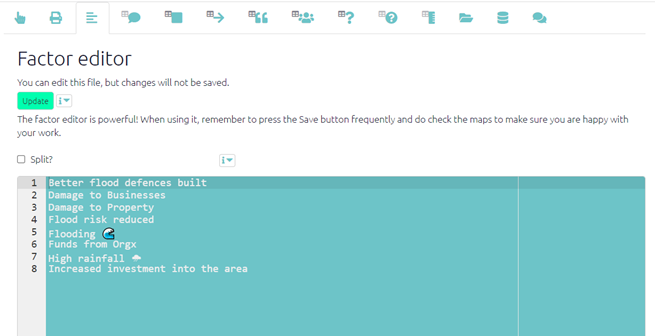
\includegraphics[width=6.77083in,height=\textheight]{_assets/image-20211007092925683.png}
\caption{image-20211007092925683}
\end{figure}

\textbf{TIP}: press Ctrl F (Cmd F on Mac) to find or Ctrl H (Cmd alt F on Mac) to replace.

\textbf{TIP}: Reformulate factor labels so that some common themes come \emph{first}.

\textbf{TIP}: Use flags like ``Problem!'' or ``\#innovation'', unique words which are easy to search for, to make it easy to find particular kinds of factor within the editor and elsewhere.

\textbf{TIP}: Merge your factors. You have two or more factors which are more or less the same?

\begin{itemize}
\tightlist
\item
  pick the best version, tweak it if necessary, and then copy the whole line
\item
  go to one of the other versions, and replace the label with the label you copied, taking care not to delete or add lines
\item
  repeat with any other similar lines, so that all the similar labels are now exactly the same
\item
  don't forget to press Update!
\item
  \ldots{} these factors with the common label will all be combined into one
\end{itemize}

Bear in mind that if you merge several factors into one, this may mean you get duplicate or triplicate links between the same pairs of factors.

\hypertarget{editing-factors-in-the-factor-editor-is-disabled-when-you-use-any-of-these-filters}{%
\section{Editing factors in the factor editor is disabled when you use any of these filters:}\label{editing-factors-in-the-factor-editor-is-disabled-when-you-use-any-of-these-filters}}

\begin{itemize}
\tightlist
\item
  combine opposites
\item
  zoom factors
\item
  remove brackets
\end{itemize}

(With these filters, it is impossible to make edits and the save button should be inactive, because any changes you made would be ambiguous.)

\hypertarget{split-recoding}{%
\section{\texorpdfstring{Split-recoding existing factors: Use the \textbf{Split} checkbox.}{Split-recoding existing factors: Use the Split checkbox.}}\label{split-recoding}}

Usually when you rename your factors, the names change everywhere. If you switch on ``Split'', each factor you rename will be split into a new factor (with the new name which is used only for the links in the current view/filter), and the original factor which is unchanged. This is useful for example if you find you have merged some ideas together too quickly into one factor and you want to split it back into two.

Suppose you have coded both ``I bought a cow''`` and ``I bought a sheep'' as \emph{bought livestock} and then you change your mind, you can go back to the statement with ``I bought a cow'', and in this tab you switch on ``Split'' and recode \emph{bought livestock} back to \emph{bought cow}. If you didn't switch on ``Split'', the other quote (``I bought a sheep'') would also be recoded as \emph{bought cow}, which isn't what you want.

The Split checkbox applies to whatever is in the current view - so you can use it to split-recode factors just within one statement, but also to split-recode factors in any filter, for example for statements from all the women, or all the sources from a particular region.

\hypertarget{advanced-editing-tips}{%
\section{Advanced editing tips}\label{advanced-editing-tips}}

\begin{itemize}
\tightlist
\item
  Go to the next mention of a selected word/sentence: \textbf{Ctrl K,or Cmd G on Mac}. Add SHIFT to these shortcuts to find the \emph{previous} mention.
\item
  Add next occurrence of selected word/sentence to multi-selection: \textbf{Ctrl-Alt-Right,or Cmd-Option-Right on Mac}. Use \textbf{Ctrl-Alt-Left / Cmd-Option-Left} to add \emph{previous} occurrence.
\item
  The app will help you consistently type words you have already used with autocomplete. Or just ignore it if you want.
\item
  Multicursor: Ctr alt Up/Down: edit multiple lines at once
\end{itemize}

\hypertarget{the-factor-editor-sidebar}{%
\section{The factor editor sidebar}\label{the-factor-editor-sidebar}}

The factor editor also has a sidebar, which shows more details for the factor currently under the cursor:

\begin{itemize}
\tightlist
\item
  The label
\item
  Any memo
\item
  Lists of influence and consequence factors

  \begin{itemize}
  \tightlist
  \item
    When hovering over the influence or consequence factors, the question\_id and quote
  \end{itemize}
\end{itemize}

\begin{figure}
\centering
\includegraphics{_assets/fe sidebar.gif}
\caption{image-20211001175928850}
\end{figure}

\hypertarget{xall-tables}{%
\chapter{⚡ All the tables}\label{xall-tables}}

From simply creating a table showing the total links to and from each factor to a visual representation of each respondent's response to a closed question. The possibilities are large - and increase with the amount of additional data your project has.

\hypertarget{tables_common}{%
\section{Features common to all the tables}\label{tables_common}}

Numerical tables are presented as \emph{heatmap tables}. The higher the number, the darker the colour of the cell will be.

\hypertarget{preset-tables}{%
\subsection{Presets}\label{preset-tables}}

If you want to keep things simple, try creating a table using one of the quick presets:

\begin{figure}
\centering
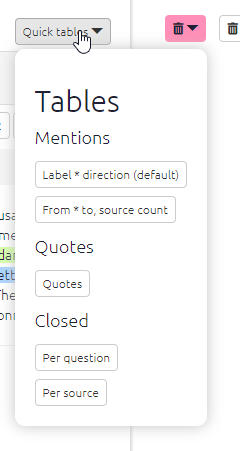
\includegraphics{_assets/image-20210914081424695.png}
\caption{image-20210914081424695}
\end{figure}

\ldots{} and the presets relevant to each table are also accessible from within that table:

\begin{figure}
\centering

\includegraphics[width=6.77083in,height=\textheight]{_assets/image-20210914081506509.png}
\caption{image-20210914081506509}
\end{figure}

\begin{center}\rule{0.5\linewidth}{0.5pt}\end{center}

\hypertarget{main-controls}{%
\subsection{Main controls}\label{main-controls}}

Each table has a set of controls, which are almost the same across all the tables.

\begin{figure}
\centering
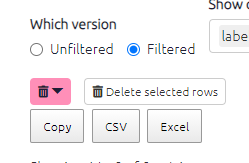
\includegraphics{_assets/image-20210914081641240.png}
\caption{image-20210914081641240}
\end{figure}

\begin{itemize}
\tightlist
\item
  When the \texttt{Which\ version} toggle is set as ``Filtered'', the tables respond to any filters you have applied in the left-hand panel of the app, just as the interactive maps do. The table shows data corresponding to the map as it is currently displayed.

  \begin{itemize}
  \tightlist
  \item
    If you want to see all the data in one table for the unfiltered map, switch this toggle to Unfiltered.
  \end{itemize}
\item
  You can copy the data from the tables into your clipboard by clicking \texttt{Copy} , and then you can then paste the data in Word or Excel to create your own tables, graphs, or visualisations.
\item
  Or save your table as \texttt{CSV} or \texttt{Excel}.

  \begin{itemize}
  \tightlist
  \item
    These buttons will export all the data in the current table, including columns which are hidden because you have not put them into the \texttt{Show\ columns} box.
  \end{itemize}
\item
  You can also screenshot the table if you prefer!
\end{itemize}

\hypertarget{adding-columns-grouping-counting}{%
\subsection{Adding columns, grouping, counting}\label{adding-columns-grouping-counting}}

You can also group the rows in the factor tables to show how the data presented differs between various respondent characteristics such as age, education, and sex. Simply select the desired filter from the Group rows filter.

When you put a field in the \texttt{count} box, your table will get an extra final column called \texttt{total}:

\begin{figure}
\centering
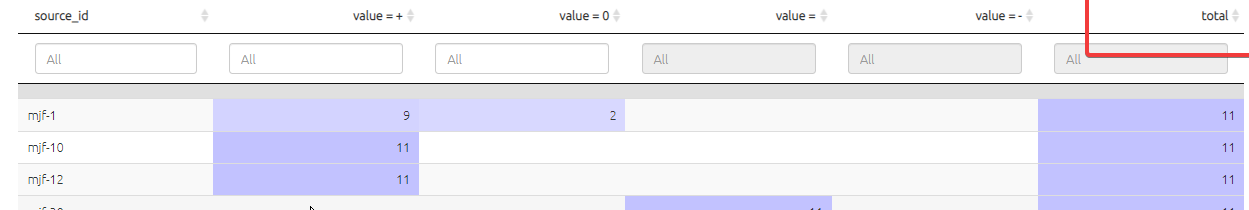
\includegraphics[width=6.77083in,height=\textheight]{_assets/image-20210914092140216.png}
\caption{image-20210914092140216}
\end{figure}

\hypertarget{search}{%
\subsection{Search}\label{search}}

You can search / filter the whole table using the box at top-right. And you can search / filter individual columns using the individual boxes. (These boxes are greyed out if all the values in the field are the same so there is nothing to search.)

\begin{figure}
\centering
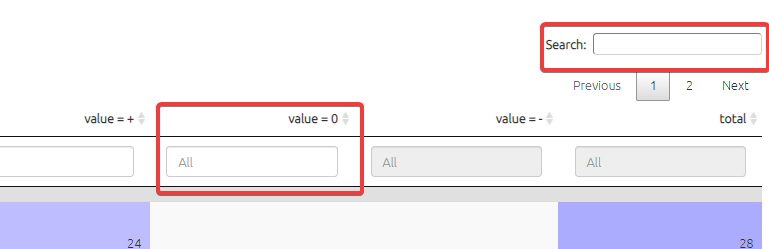
\includegraphics[width=6.77083in,height=\textheight]{_assets/image-20210914101220510.png}
\caption{image-20210914101220510}
\end{figure}

You can search a column of numbers by using the slider, or by typing an equivalent range:

\begin{figure}
\centering
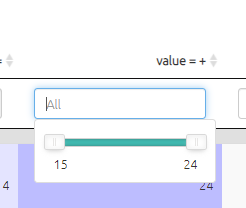
\includegraphics{_assets/image-20210914101522120.png}
\caption{image-20210914101522120}
\end{figure}

\ldots{} so if you type ``15\ldots15'' you will search just for the number 15:

\begin{figure}
\centering
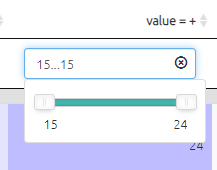
\includegraphics{_assets/image-20210914101553467.png}
\caption{image-20210914101553467}
\end{figure}

\hypertarget{sorting}{%
\subsection{Sorting}\label{sorting}}

You can sort the whole table by any column by clicking on the appropriate header:

\begin{figure}
\centering
\includegraphics{_assets/image-20210914101749080.png}
\caption{image-20210914101749080}
\end{figure}

\hypertarget{printout}{%
\section{🧪 Printout}\label{printout}}

Do you want some preformatted quotes for your report?

\begin{figure}
\centering
\includegraphics{_assets/oXugGeV2w2.gif}
\caption{oXugGeV2w2}
\end{figure}

Each table can also be shown as simple text for copying and pasting.

If you want quotes, go to the links table, click the 📘 button to display the printout, choose the columns you want. They will be shown in the Printout in the same order. Then just copy and paste.

\hypertarget{xthe-mentions-table}{%
\chapter{The Mentions Table}\label{xthe-mentions-table}}

\href{https://player.vimeo.com/video/\%5B596594094\%5D(https://vimeo.com/596594094)}{\includegraphics{Guide-to-causal-mapping_files/figure-latex/unnamed-chunk-4-1.pdf}}

This table is useful when looking at how many times factors have been mentioned in links. In the Factors table, you can display how many links are coming in and out of each factor overall, but you can't for example ask how many different \emph{sources} mentioned it, or in how many different districts.

This table loads by default with a preset; you will nearly always use this table with one of the two preset buttons at the top left. (The underlying data, which you can view if you clear the Group by and Count boxes, is a bit hard to understand, because it contains four rows for each link.)

\begin{figure}
\centering
\includegraphics[width=6.77083in,height=\textheight]{_assets/image-20211122131859032.png}
\caption{image-20211122131859032}
\end{figure}

The Direction field shows you the number of times each factors was reported as an influence factor and/or a consequence factor.

\begin{itemize}
\tightlist
\item
  From = how many times the factor was applied as an \textbf{influence} factor, i.e.~leading to another factor.
\item
  To = how many times the factor was applied as a \textbf{consequence} factor, i.e.~as a result of another factor.
\item
  Either = how many times the factor was mentioned in \textbf{either} direction.
\end{itemize}

Remember, in each case these counts depend on what you put in the Count box. You can count link\_id (which gives us the overall count, the highest number) or statement\_id, source\_id, district etc (which usually give a lower number).

The other preset \texttt{influence\ *\ consequence,\ source\ count} displays influence factors in the rows and consequence factors in the columns. As usual you can change what is counted by selecting a different field in the \texttt{Count} box.

This table is merely an overview which can help us to understand which factors are reported most frequently, and whether specific factors were more often cited as an influence or a consequence. To fully understand what the factors mean, they need to be seen in the context of the causal stories they appear in. This table can be useful for initial communication about which factor labels have been created and how often they have been applied, but do exercise caution when presenting this data as it only shows the factor in isolation, whereas when doing causal mapping we are most interested in the relationships between factors.

It is often interesting to see how many sources mentioned the factors without worrying about the direction, i.e.~whether they were mentioned as influence or consequence. That's what the ``Source counts'' preset is for. This uses the field \texttt{mentions} which is frankly a bit of a hack, as it only has one value, namely ``any'', but it serves to construct the table we wanted:

\begin{figure}
\centering
\includegraphics[width=6.77083in,height=\textheight]{_assets/image-20211122133447831.png}
\caption{image-20211122133447831}
\end{figure}

\hypertarget{xthe-factors-table}{%
\chapter{The Factors table}\label{xthe-factors-table}}

The factors table presents the factors applied during coding. There are columns for label, factor memo, and columns for any other fields you have provided, maybe ``domain'' for instance. The app also calculates some additional fields like:

\begin{itemize}
\tightlist
\item
  \texttt{betweenness} (how central is the factor in the map?)
\item
  \texttt{in\_degree} (how many links come in to this factor?)
\end{itemize}

This table is an overview which can help us to understand which factors are reported most frequently, and to view and understand metadata like memos. As usual, this table responds to any filters you have applied on the left-hand side and can be additionally sorted and filtered.

\hypertarget{xfactormemos}{%
\section{Factor memos}\label{xfactormemos}}

Factor memos are an important part of your Codebook. They appear:

\begin{itemize}
\tightlist
\item
  when you hover in interactive view
\item
  in the sidebar in the factor editor
\item
  in the factors table.
\end{itemize}

You can create and edit the memos from interactive view:

\begin{figure}
\centering
\includegraphics[width=6.77083in,height=\textheight]{_assets/edit.gif}
\caption{image-20211001175928850}
\end{figure}

\ldots{} or from the factors table:

\begin{figure}
\centering
\includegraphics[width=6.77083in,height=\textheight]{_assets/factors-table.gif}
\caption{image-20211001175928850}
\end{figure}

\hypertarget{xthe-links-table}{%
\chapter{The Links Table}\label{xthe-links-table}}

This table counts factors differently to the mentions table as it counts links rather than individual factor mentions. Each row represents one link and has columns for that link's influence factor and consequence factor, as well as many other columns. This table is also linked to the \protect\hyperlink{xthe-statements-table}{statements} and \protect\hyperlink{xthe-sources-table}{sources} tables. Use this table to show the links between factor labels. Information like the related quote is also available in this table, the easiest way to view this is to select the quotes preset.

\begin{figure}
\centering
\includegraphics[width=6.77083in,height=\textheight]{_assets/image-20211122150602045.png}
\caption{image-20211122150602045}
\end{figure}

\hypertarget{fields}{%
\subsection{Fields}\label{fields}}

\begin{itemize}
\tightlist
\item
  \texttt{from}. Contains numbers which match the factor\_ids of the factors.
\item
  \texttt{to}. Contains numbers which match the factor\_ids of the factors.
\item
  \texttt{statement\_id}. Contains numbers which match the statement\_ids of the statements.
\item
  \texttt{link\_memo}. For making notes about a link as you code.
\item
  \texttt{hashtags}. \protect\hyperlink{xhashtags}{Re-usable tags} which are usually common across several links, for example \#hypothetical or \#certain or \#check.
\end{itemize}

\hypertarget{xthe-statements-table}{%
\chapter{The Statements Table}\label{xthe-statements-table}}

This table makes searching for a specific statement easy. By clicking on a row in this table you will jump straight to the statement, meaning you can edit the associated factors in the left-hand-side panel. This table shows you all the statements in your map file. You can use the search bars to look for statements by their id or by a word/phrase in the text.

\begin{figure}
\centering
\includegraphics[width=6.77083in,height=\textheight]{_assets/image-20211122152257053.png}
\caption{image-20211122152257053}
\end{figure}

\hypertarget{fields-1}{%
\subsection{Fields}\label{fields-1}}

\begin{itemize}
\tightlist
\item
  \texttt{statement\_id}. A running number from 1 upwards.
\item
  \texttt{source\_id}. A code which matches the field \texttt{source\_id} in the \texttt{sources} table.
\item
  \texttt{question\_id}. A code which matches the field \texttt{question\_id} in the \texttt{questions} table.
\item
  \texttt{statement\_memo}. For making notes about a statement as you code.
\end{itemize}

\hypertarget{xthe-sources-table}{%
\chapter{The Sources Table}\label{xthe-sources-table}}

\href{https://player.vimeo.com/video/596519456}{\includegraphics{Guide-to-causal-mapping_files/figure-latex/unnamed-chunk-5-1.pdf}}

The sources table, when they are no filters applied, simply lists all of the respondents and any additional data collected about them (sex, age, location, education.) It also shows the interview type (individual or focus group) for each source. When filters are applied, the table will only present the relevant sources/respondents. If you are searching and filtering for a specific factor, this table will update and only show sources who reported that factor.

This table can be useful to check that all the sources have been imported into the app correctly. The table also provides a summary of the respondents which can be useful for presenting respondent demographics in the report, either in the sampling section or as an appendix.

\begin{figure}
\centering
\includegraphics[width=6.77083in,height=\textheight]{_assets/image-20211122152944416.png}
\caption{image-20211122152944416}
\end{figure}

\hypertarget{fields-2}{%
\subsection{Fields}\label{fields-2}}

\begin{itemize}
\tightlist
\item
  \texttt{source\_id}. A code which matches the field \texttt{source\_id} in the \texttt{statements} table.
\item
  \texttt{source\_memo}. For making notes about a source as you code.
\item
  Any other fields which you have imported.
\end{itemize}

\hypertarget{xthe-questions-table}{%
\chapter{The Questions Table}\label{xthe-questions-table}}

This table displays the text and ID for every question included in the questionnaire. It may also show any other additional data fields which are the same for each question, e.g.~questionnaire subsection or question group.

\begin{figure}
\centering
\includegraphics[width=6.77083in,height=\textheight]{_assets/image-20211122153204078.png}
\caption{image-20211122153204078}
\end{figure}

You may wish to include this table as an appendix in your report or as a reference point for looking up particular questions.

\hypertarget{xthe-closed-question-blocks-table}{%
\chapter{The Closed Question Blocks Table}\label{xthe-closed-question-blocks-table}}

\href{https://player.vimeo.com/video/596497752}{\includegraphics{Guide-to-causal-mapping_files/figure-latex/unnamed-chunk-6-1.pdf}}

There are two tables which provide a summary of the responses to the \textbf{closed questions} asked at the end of each QuIP questionnaire domain. The following symbols are used in the tables to represent the direction of change indicated by the response to the closed question:

\begin{longtable}[]{@{}lll@{}}
\toprule
\textbf{Symbol} & \textbf{Direction of change} & \textbf{Example responses} \\
\midrule
\endhead
\textbf{0} & No change & ``No change'' ``Stayed the same'' \\
\textbf{+} & Positive change & ``Better'' ``Improved'' ``Increased'' \\
\textbf{-} & Negative change & ``Worse'' ``Decreased'' \\
\bottomrule
\end{longtable}

The closed questions table gives an overview of how each \textbf{individual} respondent answered each closed question. The closed question summary table presents the \textbf{total respondent counts} for each direction of change. For every closed question you can see how many respondents reported positive, negative, or no change in that domain. You may wish to search and filter the statements to view only the closed question responses from a particular respondent group.

Why would I use this table?

These tables provide a snapshot of the overall trends of change across the domains, so they can be a helpful introduction and ``easing in'' to the findings - before diving deeper into the causal stories! The closed question responses can also provide interesting insights when compared to the open-ended responses, especially in cases where they might differ.

A full list of closed question responses can be found \href{https://guide.causalmap.app/importing-your-data-special-cases.html?q=recodes\#quip-recodes-for-closed-questions---live-link}{here}.

You can also add other additional data fields like respondent gender:

\begin{figure}
\centering
\includegraphics[width=6.77083in,height=\textheight]{_assets/image-20211008095846116.png}
\caption{image-20211008095846116}
\end{figure}

\hypertarget{xmetrics}{%
\chapter{The Metrics Table}\label{xmetrics}}

\hypertarget{summary}{%
\section{Summary}\label{summary}}

The metrics table displays a range of useful measurements about your data. These metrics respond to any filters that have been applied to your data, so consider whether you want to see these metrics \texttt{unfiltered} or \texttt{filtered}.

\begin{figure}
\centering
\includegraphics[width=6.77083in,height=\textheight]{_assets/WTcXlasgYI.gif}
\caption{WTcXlasgYI}
\end{figure}

\hypertarget{what-the-metrics-mean}{%
\section{What the metrics mean}\label{what-the-metrics-mean}}

There are quite a few metrics, some are more self-explanatory than others. The table below expands on the brief description given in the metrics table.

\begin{longtable}[]{@{}
  >{\raggedright\arraybackslash}p{(\columnwidth - 2\tabcolsep) * \real{0.14}}
  >{\raggedright\arraybackslash}p{(\columnwidth - 2\tabcolsep) * \real{0.86}}@{}}
\toprule
\begin{minipage}[b]{\linewidth}\raggedright
Metric
\end{minipage} & \begin{minipage}[b]{\linewidth}\raggedright
\textbf{Explanation}
\end{minipage} \\
\midrule
\endhead
\textbf{size} & The total number of links in the map. \\
\textbf{order} & The total number of factors in the map. \\
\textbf{links\_per\_factor} & The average number of links per factor. Usually, you want to have plenty of links per factor. \\
\textbf{n\_statments} & The number of statements in the map. \\
\textbf{n\_words} & The total number of words in all the statements. \\
\textbf{n\_coded\_words} & The number of words in coded phrases. \\
\textbf{n\_characters} & The number of characters in all statements. \\
\textbf{links\_per\_statement} & The number of links per statement. \\
\textbf{percent\_coded} & The percentage of statements which have been coded. \\
\textbf{adhesion} & The minimum edge connectivity or line connectivity. The minimum number of edges that if you deleted them would result in a disconnected map. If you have a disconnected map already, like most maps are, that number will be 0. However, if you have a map which loops, and all factors are both consequence and influence factors, that number will be 1. \\
\textbf{component\_count} & The number of unconnected components in the map. Do you have islands in your map? The app first identifies the components -- sets of factors which are all (``weakly'', i.e.~ignoring the direction of the links) connected to each other by some path; then counts how many separate components there are, i.e.~none of the factors in one component are connected to any of the factors in the other component(s). \\
\textbf{diameter} & The length of the longest geodesic or path between two factors. For example, the count for A-\textgreater B-\textgreater C-\textgreater D would be three as it's three links from A to D. This takes into account the direction of the arrows. \\
\textbf{reciprocity} & The proportion of mutual connections in the map. This calculates the proportion of factors in which both factors influence one another. The connection must be between two factors, feedback loops are not counted. \\
\textbf{min\_cut} & The minimum number of links that you would have to remove to split the map into two clusters. \\
\textbf{mean\_dist} & The mean number of links between all factors in the map. \\
\bottomrule
\end{longtable}

\hypertarget{xdata-manager}{%
\chapter{Data manager}\label{xdata-manager}}

This page gives you useful information about your mapfile. Ideally you want the page to look like the screenshot below, with all information in the relevant table. It is good to check this page to ensure your data is in the correct place, especially after you have \protect\hyperlink{ximport}{uploaded your data}.

\begin{figure}
\centering
\includegraphics[width=6.77083in,height=\textheight]{_assets/image-20211206102018607.png}
\caption{image-20211206102018607}
\end{figure}

\hypertarget{the-updates-panel}{%
\chapter{The Updates panel}\label{the-updates-panel}}

In this panel, you can see updates about all the files you have access to.

With the toggle at the top, you can select whether to show:

\begin{itemize}
\tightlist
\item
  The most recent status for each file
\item
  All updates for the currently loaded file
\item
  All updates for all files
\end{itemize}

You can also click on a row to load the corresponding file.

\begin{figure}
\centering
\includegraphics[width=6.77083in,height=\textheight]{_assets/file manager screenshot-16376049547992.png}
\caption{file manager screenshot}
\end{figure}

\hypertarget{part-creating-maps}{%
\part{Creating maps}\label{part-creating-maps}}

\hypertarget{top-tips}{%
\chapter{⚡Top tips if you have just starting coding}\label{top-tips}}

First of all, there's nothing to worry about, it's fun!

The versioning / backups feature is amazing so you can always go back to any version of your file at any earlier time point.

Also, the \protect\hyperlink{factor-editor}{Factor Editor} makes it easy to rapidly change one or many factors. And you can do it either globally, i.e.~changing one factor everywhere in the file, or you can do it for particular statements, if you press the Split checkbox.

Zoom your browser out so everything fits on your screen. Try pressing Ctrl 0 or Cmd 0 to get normal view, then press Ctrl - or Cmd - once or twice if your eyes can stand it.

Don't forget you can get more space while coding by pressing the little resize arrow at the top between left and right panels.

Don't forget you can see additional information about each statement, and make memos on the statement or the source by clicking the info toggle. \includegraphics[width=6.77083in,height=\textheight]{_assets/image-20211220153222953.png}

Normally you'll want to keep the Filters panel closed because it takes space.

Don't bother coding the same link more than once for the same source, unless they bring up distinctively different evidence each time.

It's okay not to code a statement at all. If there's nothing in it, or if people are just making vague and general statements.

You'll find you're constantly shifting between sometimes creating new factors, and then going back and reviewing them and merging them and organising them in the \protect\hyperlink{factor-editor}{Factor Editor}.

Don't forget you can combine two or more factors into one. Just by pasting the same label over all of them.

Don't forget when you want to search rapidly through already coded links through all of the statements, you can click on the rows in the \protect\hyperlink{the-links-table}{links table} or the \protect\hyperlink{the-statements-table}{statements table}. To go back to the relevant statements directly.

Don't forget that the app always knows what question a particular link is in response to, so you don't need to try to sneak the question information somehow into the factors and links, unless you want to.

Occasionally, someone will make a comment about something which is worth coding, even though there isn't actually a causal link. For example, they might make general comments about some outcome without saying what causes it. In this case just make a link like (no influence factor) --\textgreater{} some outcome. (But if you find you are doing this a lot, you might need to rethink your research design.)

Don't forget while coding you can view the map from the One statement view or the Many statement view.

If you are using \protect\hyperlink{xhierarchical-coding}{hierarchical/nested coding} (and you probably should) don't forget you can see the whole map zoomed out to the top level: just press the appropriate button in the Filters panel.

\hypertarget{creating-good-factor-labels}{%
\chapter{📚 Creating good factor labels}\label{creating-good-factor-labels}}

\href{https://player.vimeo.com/video/580212681}{\includegraphics{Guide-to-causal-mapping_files/figure-latex/unnamed-chunk-7-1.pdf}}

Remember that in general, factor names are case sensitive. So the app will not treat `funding' and `Funding' as the same.

You can use emojis 😍 and other special characters in your factor labels.

Also, semi-colons `;' you can use them if you want, but note that the app will then treat this factor label as \protect\hyperlink{xhierarchical-coding}{hierarchical}.

\hypertarget{actor-focused-labels}{%
\section{Actor-focused labels}\label{actor-focused-labels}}

Often you will find that it is easier and clearer if you formulate your labels to highlight who does what. So a formulation like ``advocacy on renewables'' might be better as ``NGOs conduct advocacy campaign on renewables''. If you do this, you may even find that you want to break this up into different actors, for example ``\textbf{NGOs} conduct advocacy campaign on renewables'' and ``\textbf{Politicians} pay more attention to renewables''. In particular, avoid using passive formulations like ``Advocacy is carried out'' or ``Awareness is raised''.

\hypertarget{formulating-factors-as-semi-quantitative}{%
\section{Formulating factors as ``semi-quantitative''}\label{formulating-factors-as-semi-quantitative}}

\hypertarget{relax-use-heterogeneous-in-vivo-factor-labels}{%
\subsection{Relax! Use heterogeneous, ``in-vivo'' factor labels}\label{relax-use-heterogeneous-in-vivo-factor-labels}}

It might be tempting to try to formulate all factor labels in a strictly similar way, using for example language like ``increased probability of \ldots{}'' or ``positive change in \ldots{}'' in every case. But it is difficult to identify and agree on a satisfactory template for doing this which will capture enough of the way people really make causal explanations (in the way that quantitative social scientists hope to measure everything just with continuous variables). This is always a balancing act, but we encourage you when in doubt to stick fairly close to the actual language your sources use (so-called ``in-vivo'' coding), and don't be \emph{too} worried if your factor labels are different from one another grammatically (e.g.~some express a difference like ``improvement in X'' and some do not.

The formulation of \textbf{factor labels} should fit the intended interpretation of the \textbf{causal links}. For example, most commonly B ➜ E is supposed to mean that B exerts in some sense an ``increasing'' or ``decreasing'' influence on E, then both B and E need to be formulated in a corresponding way. In order to ease interpretation, with a few exceptions, factors should be labelled and understood in such a way that it makes sense to say ``more of this'' or ``this happened as opposed to not happening'': we call these semi-quantitative factors.

Consequently you should avoid a factor label like Training courses, which might be understood as a mixed bag of various causal factors to do with training courses. We would usually prefer a label such as Training courses delivered or Quality of training courses which are easier to understand as things which can increase or decrease, or happen or not happen. You may even prefer to use labels like Quality of training courses improved or Improved quality of training courses, in which the \emph{difference made} is already included in the title.

\hypertarget{quip-specific-back-chaining}{%
\subsection{QuIP specific: back-chaining}\label{quip-specific-back-chaining}}

In QuIP projects, most of the interview material comes in response to questions about changes in the reference period, usually the last three years. QuIP questioning continues back up the causal chain, asking what was the reason for that? \ldots{} and the reason for that? That means that most influence factors will also be expressed as changes or differences (a change in F is explained by a change in E which is explained by a change in D\ldots.), whereas some are not (e.g.~``unemployment''). Some analysts will try to avoid coding this kind of claim (can something which has been around a long time explain a change in the last three years?) but you may decide that this distinction does not matter too much. If something really does describe a \emph{change} (e.g.~``became unemployed'') then it should be coded.

Most QuIP testimony begins with questions about whether things have got better or worse, so most causal factors, going back up the causal chain, are likely to be semi-quantitative too.

\hypertarget{examples-of-semi-quantitative-factors}{%
\subsection{Examples of semi-quantitative factors}\label{examples-of-semi-quantitative-factors}}

These are examples of factor labels where you can judge whether it happened more or less, whether it is higher or lower, or whether it happened versus not happened:

\begin{itemize}
\tightlist
\item
  Sold cow
\item
  Earthquake happened
\item
  (Had) good harvest
\item
  (Level of) bank account
\item
  (Level of) ethnic tolerance
\item
  Quality of seeds
\end{itemize}

In some contexts, we can also talk about the \emph{likelihood} of events, so ``if people get a good harvest they are less likely to sell their cow.''

It is also perfectly acceptable and sometimes necessary to use purely qualitative labels, e.g.~coping style, \href{https://guide.causalmap.app/creating.html\#examples-of-non-quantitative-factors}{see below}. However, this may limit some of the analysis and reporting tools available.

\hypertarget{opposed-pairs-of-causal-factors}{%
\section{Opposed pairs of causal factors}\label{opposed-pairs-of-causal-factors}}

What to do when some explanations use a causal factor phrased in a positive way and others use a similar causal factor but phrased the other way around?

``I feel good because my health is good.''

``My sister lost her job because her health is bad.''

We could code these:

Health improved ➜ Feel good

Health got worse ➜ Lost job

But we might feel we are missing the fact that the first factor in each case is arguably the same thing, just the other way around.

Solution 1: do nothing

This may mean you find yourself using pairs of opposing factors such as Better health and Worse health to capture the causal claims -- things which are in a sense the opposite of one another. You might decide that is fine anyway, because you are happy to have pairs of factors like this, or because you decide that the pair of factors are not really polar opposites at all and therefore you don't want to combine them. For example, illness is arguably not really simply the opposite of health but a quite different state with its own causal rules.

Solution 2: merge them

If you use more advanced coding styles involving ``strength,'' detailed in the ``Extra'' section of this Guide, you can avoid this by just using one factor like Better health.

Alternatively, `Health Improved' and `Health got Worse' could be coded as `Health Improved' and `\textasciitilde Health Improved' respectively, with `\textasciitilde{}' indicating the `opposite' of an improvement in health. The app will then treat links to Health Improved and \textasciitilde Health Improved separately. \href{https://guide.causalmap.app/coding-opposites.html\#combining-opposites}{More information on this can be found here.}

\hypertarget{formulating-factors-as-desirable}{%
\section{Formulating factors as desirable}\label{formulating-factors-as-desirable}}

If possible, especially when conducting evaluations or research for policy purposes, try to formulate these semi-quantitative factors so that for each one, \emph{more} of it can be broadly thought of as \emph{more desirable}, e.g.~Health, Wellbeing; and failing that, as something \emph{undesirable}, e.g.~Psychosocial Stress, Mortality. Including factors which primarily code something undesirable as well as factors which primarily code something desirable, is often very natural, but you might sometimes have to think more carefully when making reports and summaries.

Again, it is least useful, but also perfectly acceptable and sometimes necessary, to fall back to using factor labels which are ambiguous as to their desirability, e.g.~Moved house\emph{,} if there is a lack of information or in the case of factors which simply are neutral.

\hypertarget{examples-of-non-quantitative-factors}{%
\section{Examples of non-quantitative factors}\label{examples-of-non-quantitative-factors}}

These are examples of factors where it is very hard to quantify the occurrence in any way:

\begin{itemize}
\tightlist
\item
  Teaching style
\item
  Coping strategy
\item
  The content of the report
\end{itemize}

We call these non-quantitative factors. We might try to reword them as semi-quantitative factors like this:

\begin{itemize}
\tightlist
\item
  Helpfulness of teaching style
\item
  Positiveness of report
\end{itemize}

The diagram below is an acceptable causal map, even though the intervening two variables are an example of more qualitative rather than (semi-)quantitative labels. It tells us that the training did something to the teaching style, which did something relevant to the learning style, which improved student outcomes. We don't have a theory about the ``how'' of any of the arrows, and we don't (necessarily) suggest that teaching style or learning style are things which can be measured on a single scale from e.g.~``less'' to ``more.''

\hypertarget{using-flags-in-factor-labels}{%
\section{Using flags in factor labels}\label{using-flags-in-factor-labels}}

Hierarchical coding is one way to structure your coding. However, sometimes you don't want to think in terms of a strict hierarchy, or maybe you have an additional set of themes which cut across that hierarchy.

Flags are useful in either of these cases.

Flags are just sequences of characters within a factor label to which you have given a special meaning, and which are unique and easy to search for. These can include letters, emojis or phrases. You can do coding without any such flags if you want, but it can help when searching and filtering.

A quote like ``family situation is better now because of improved food availability'' can be coded like this:

\begin{quote}
More food --\textgreater{} Improved wellbeing
\end{quote}

Now, maybe you are asked also to keep track of any aspects of the project which have to do with nutrition. Nutrition is not really part of your system of factors, but you would like to be able to construct some maps just to look at this aspect. So you can write this:

\begin{quote}
More food \#nutrition --\textgreater{} Improved wellbeing
\end{quote}

Similarly, if Improved Wellbeing is one of the desired outcomes of the project, we might want to reflect that by adding a flag ``(Outcome)'' like this.

\begin{quote}
More food --\textgreater{} Improved wellbeing (Outcome)
\end{quote}

Then we can easily search for this and other desired outcomes.

A flag like ``men'' is not suitable because it is likely to appear elsewhere (e.g.~as part of ``women'' or ``management''). To get round this, add additional characters like a hash: ``\#men''; this makes the flag unique.

If you use curved or square brackets around your flags, you can use one of the app filters to hide the flags for specific maps if desired.

\hypertarget{xhanging-flags}{%
\subsection{Hanging flags}\label{xhanging-flags}}

A subtle trick is to use hanging flags which are additional hierarchical components. So rather than writing, say,

\begin{quote}
More food \#nutrition --\textgreater{} Improved wellbeing
\end{quote}

you write

\begin{quote}
More food; \#nutrition --\textgreater{} Improved wellbeing
\end{quote}

(note the \texttt{;} ), then if you ``zoom out'' to the top level of the hierarchy, the flag will be neatly hidden:

\begin{quote}
More food --\textgreater{} Improved wellbeing
\end{quote}

\hypertarget{flags-for-bundling-factors}{%
\subsection{Flags for bundling factors}\label{flags-for-bundling-factors}}

It is very convenient to use flags when you want to \protect\hyperlink{bundlefactors}{bundle factors}. This means you can easily collapse together one or more sets of factors sharing a common theme, regardless and independently of any hierarchical structure you are using.

\hypertarget{intervention-flags}{%
\subsection{Intervention Flags}\label{intervention-flags}}

The commissioner of an evaluation will nearly always want to be able to focus on their own interventions, so it is advisable to use a consistent label or category across all factors which are noted as project inputs in order to be easily searchable. These will usually be influence factors with no parents, i.e.~factors which have no incoming influence factors.

In the example below, both are similar interventions, but one is clearly attributable to an NGO.

``MSF gave us medicines which healed the children''

MSF gave medicines --\textgreater{} children healed

``Someone gave us medicines which healed the children''

Unknown actor gave medicines --\textgreater{} children healed

You have a range of options to flag this difference in the label and enable you to filter for all project-related interventions once the data is coded.

· All such interventions can be labelled with the NGO's name

· If you are doing nested coding, you can nest such factors within a higher-level factor like `Interventions;'

· And/or you can use a specific intervention flag, e.g.~\#Intervention. (QuIP has its own flags, {[}I{]} for Implicit and {[}E{]} for Explicit).

You can use any label you want as long as you are sure it is unique, it doesn't appear accidentally in other factor names, and you use it consistently.

\hypertarget{outcome-flags}{%
\subsection{Outcome Flags}\label{outcome-flags}}

Similarly, if you wish to flag up outcomes /consequences as either desired/desirable/valued, or the inverse, you can mark these in a way which makes them easy to identify. You could use symbols like ♥ etc. in the labels to designate this, or use use QuIP-style labels {[}P{]} for positive and {[}N{]} for negative. This can be helpful when undertaking analysis; for example, displaying direct and indirect links from some or all of the intervention factors to some or all of the positive outcome factors or highlighting or counting paths leading to all negative outcome factors, etc.

Again, you can use any label you want as long as you are sure it is unique, it doesn't appear accidentally in other factor names, and you use it consistently.

\hypertarget{coding-your-statements-in-context-referring-to-evidence-from-elsewhere}{%
\subsection{Coding your statements in context: referring to evidence from elsewhere}\label{coding-your-statements-in-context-referring-to-evidence-from-elsewhere}}

When coding data from an interview it is very important to see the whole interview as your source, and not fall into the trap of only coding the statement in front you, out of context. If your statements are split into separate questions (as is often the case with QuIP), it can be misleading to code just one statement in isolation, without taking account of what the respondent says earlier or later in the interview. For this reason we recommend that all analysts read the whole interview before starting to code, and start to formulate causal stories which fit across the whole interview. In some cases, you may prefer to have the whole interview as one statement, and to code it all in one place. This is absolutely possible, and just depends how the data is imported (whatever information is on one row in the .csv file is considered a statement). If, however, the interview is too long, or you would still prefer to code question by question, you need may want to refer to information provided in another statement when coding a link. This is not necessary but can be useful when sharing the file with a commissioner who may look at quotes associated with links, and not understand the rationale for coding without further context. The same applies for different parts of a paragraphs within one statement; you may want to highlight two separate parts of a longer statement.

If the quote is not exactly verbatim in the statement, the app won't let you save anything. (If this happens, just cancel the quote (press the X) and start again.) The app is really picky about this to ensure your quotes are accurate. However, this rule does not apply for anything between square brackets, a useful feature for this case. If the evidence for a link is mentioned in two different parts of a single statement, like this:

\emph{Yes, we got the help from OrgX. Sed ut perspiciatis unde omnis iste natus error sit voluptatem accusantium doloremque laudantium, totam rem aperiam, eaque ipsa quae ab illo inventore veritatis et quasi architecto beatae vitae dicta sunt explicabo. And because of that help, now I have a job. qui dolorem ipsum quia dolor sit amet, consectetur, adipisci velit. Ut enim ad minima veniam.}

You can use square brackets to remove the text you don't want. Highlight the whole piece of text you want to code, and then edit the quote in the quote window, replacing what you don't need with {[}\ldots{]}

\emph{Yes, we got the help from OrgX. {[}\ldots{]} And because of that help, now I have a job.}

Be careful not to introduce any new text or even spaces.

You can also use the same technique to add your own comment or quote from a statement elsewhere in the interview:

\emph{{[}this is my note{]} Neque porro quisquam est, qui dolorem ipsum quia dolor sit amet, consectetur, adipisci velit, sed quia non numquam eius modi tempora incidunt.}

Ellipses are also helpful to refer to another statement as part of your evidence:

\emph{{[}reference to statement 36: The whole village received help from Org X{]} Thanks to that help we received, we are now growing our own produce.}

\hypertarget{consolidating-and-editing-factor-labels}{%
\section{Consolidating and editing factor labels}\label{consolidating-and-editing-factor-labels}}

After you have created more than about 50 factors you will probably feel the need to start consolidating and renaming them and perhaps merging some.

If you look at the Mentions table in the app, you will probably find a lot of \emph{pairs} of factors each of which is used only once, as half of this particular pair, and don't appear linked into longer stories. We almost certainly will want to consolidate some of these factors by in some way merging them with others which have similar meaning.

Suppose you have 100 factors which are just mentioned once or twice. It's a lot of work to do all that coding, a lot of work for almost nothing, because those very infrequent factors (we call them ``tiddlers'') are unlikely to appear much in any reporting you do. With hierarchical coding, even infrequent factors can contribute to the bigger picture.

Before we even think about consolidating factors, do remember the golden rule that, \textbf{when coding a new link, always look at your existing factors and try selecting one of those before creating a new one.} Even if you think an existing factor isn't quite a perfect fit, you can use it and adjust the factor name later. Ideally you will always be able to think of labels for your factors which are at least general enough to cover a few different cases.

It can be helpful to reformulate factor labels so that some common themes come \emph{first}:

\begin{itemize}
\tightlist
\item
  ``communication difficulties - intercultural''
\item
  ``communication difficulties - lack of internet''
\end{itemize}

This is useful when the factors are listed alphabetically and can be a stepping-stone to formulating factors hierarchically.

Even when doing inductive coding, some people formulate factors with a theory in mind, with some higher-level factors like ``communication difficulties'' or ``resilient outcomes.'' However we have found that it is often most interesting when you let the theory emerge rather than by starting with a preconceived template in this way. Look at your factors periodically as you code and see if there are any obvious groups.

Also, our recommended way of having your cake and eating it - keeping the detail but seeing the general trends too -- is ``hierarchical coding.'' \href{https://guide.causalmap.app/creating.html\#simplifying-causal-maps-with-hierarchical-coding}{See below}.

\hypertarget{merging-multiple-factors-into-one}{%
\subsection{Merging multiple factors into one}\label{merging-multiple-factors-into-one}}

In some cases you will simply decide, in the face of too many factors, to merge \texttt{Engagement\ with\ communities} and \texttt{NGO\ engagement}into one, e.g.~\texttt{Engagement}.

If you have two factors like this which are very similar but not quite the same, you can sometimes keep some detail by using a composite label which explicitly mentions both i.e.\texttt{Engagement\ with\ communities/NGOs}.

\hypertarget{xedit-factor-and-links}{%
\chapter{Editing factors and links}\label{xedit-factor-and-links}}

It is likely that you will need to regularly review and edit your links, and there are various ways to do this in the app. You can also delete factors and links in the same way, however you cannot delete factors or links when certain filters are applied such as \texttt{combine\ opposites} and \texttt{zoom} as these filters represent multiple factors as one factor label.

\textbf{Editing links in the interactive tab}

Click on the link you want to change in the interactive view. Make any adjustments in the left panel, e.g.~change the influence factor (in the first box), and/or the consequence factor (in the second box). You can change the quoted text just by re-highlighting the correct passage in the statement panel above in the same way that you made the original highlight. Press the green Save button to finish editing.

\begin{figure}
\centering
\includegraphics[width=6.77083in,height=\textheight]{_assets/image-20211206150101705.png}
\caption{image-20211206150101705}
\end{figure}

\textbf{Editing factors in the interactive tab}

To edit your factor labels in the interactive view, just click on the factor and then `edit factor' to open the edit panel. Using this panel you can change the text of the individual factor or add a memo.

\begin{figure}
\centering
\includegraphics[width=6.77083in,height=\textheight]{https://bathsdr.org/wp-content/uploads/2021/11/Picture1.png}
\caption{img}
\end{figure}

\textbf{Edit factors in the Factors table}

To edit factors in the edit factors table, click on the row containing the factor you would like to alter. This will open the edit panel, as shown above. You can use the search function at the top of the factors table to find the factor you want to change.

\textbf{Edit factors and links in the Links table}

In the links table you can edit links and factors by clicking on the row containing the text you want to edit, this will open a panel asking what you want to do with this link. By clicking `edit interactive' in this panel you will be able to edit the link in the left-hand side panel, where you originally coded the statement.

\begin{figure}
\centering
\includegraphics[width=6.77083in,height=\textheight]{https://bathsdr.org/wp-content/uploads/2021/11/chrome_DjCOFel9yz.png}
\caption{img}
\end{figure}

You can also edit multiple factors using the \protect\hyperlink{xfactor-editor}{factor editor tab}.

\hypertarget{simplifying}{%
\chapter{📚 Simplifying causal maps with hierarchical coding}\label{simplifying}}

\hypertarget{summary-1}{%
\section{Summary}\label{summary-1}}

You can use a separator like ; to create nested factor labels, like this:

New intervention; midwife training ➜ Healthy behaviour; hand washing

We can read this separator as ``in particular'' or ``for example'':

New intervention, in particular the midwife training,

Or we can read it in reverse like this:

The midwife training, which is an example of / part of the new intervention

Factor labels can be nested to any number of levels, e.g.

New intervention; midwife training; hand washing instructions

The higher level factors can, within the same coding scheme, themselves be used for coding, e.g.~we could code ``this whole new intervention has also led to happier health providers'' like this:

New intervention ➜ Happier health providers

We can ``zoom out'' of a causal map containing nested factors to show a simpler, higher-level structure as a summary. This is done by re-routing links to and from the lower-level factors into their higher-level parents.

So then, loosely yet informatively and with certain caveats, accepting a loss of detail but affirming that the overall meaning is not distorted, we can deduce from the first example above the following causal map:

New intervention ➜ Healthy behaviour

Usually these higher-level factors will each be summaries of many lower-level factors.

\hypertarget{introduction}{%
\section{Introduction}\label{introduction}}

An analyst coding text to create a causal map is confronted with the same challenge as any qualitative researcher: identifying recurring themes in such a way as to help a larger picture emerge, while retaining important detail. Expressing factor labels in a hierarchical fashion can help solve this problem. But hierarchical labelling also enables a particular strength of causal mapping: it lets us ``zoom out'' to view a whole causal map from a higher-level perspective, merging causally similar concepts to give a simpler map with far fewer components. Formally, the process of zooming out produces a map which logically \emph{follows} \emph{from}, is \emph{implied by}, the original map. This chapter also introduces a smarter way to ``zoom out'' from a causal map, and explains how these features are implemented in the Causal Map app.

When conducting qualitative coding of any text, there is always a tension between wanting to keep the detail (e.g.~hand washing) but also to code in such a way that general themes emerge (e.g.~health behaviour). One way to do this is to organise the codes into a hierarchical structure, so that ``Hand washing'' is nested as part of ``Health behaviour''. This can be done (see e.g.~Dedoose, saturateapp.com) by using labels in which the hierarchy is directly expressed, for example ``Hand washing; health behaviour'' -- using semi-colons or some other convenient character to separate the levels of the hierarchy.

This approach is convenient for several reasons:

\begin{itemize}
\item
  A search for ``Health behaviour'' will find Health behaviour; Hand washing as well as Health behaviour; vaccinating children and other combinations.
\item
  It can be arbitrarily extended to any number of levels, e.g.~Health behaviour; Hand washing; Before meals
\item
  Related items appear next to each other when they are listed alphabetically
\item
  The hierarchical structure does not require that the analyst (whether using paper-and-pencil or software) maintains a separate set of ``parent'' codes; the higher-level codes are simply whatever is visible before the semi-colons. Higher-level codes can be created and changed on the fly without having to open a separate codebook or software interface.
\item
  It is possible to code directly at higher levels, for example using the code Health behaviour where no more details are given.
\end{itemize}

When reading a nested factor label aloud, the semi-colons could be substituted with ``\ldots{} and in particular \ldots.'', e.g.~``Health behaviour, and in particular Hand washing, and in particular Before meals''.

The way factor (labels) emerge during causal mapping is just a special case of the way codes emerge in any qualitative coding process, and nested coding is useful in ordinary qualitative data analysis as well as in causal mapping. However, hierarchical coding in causal mapping is particularly exciting because it allows us to do things like simplify a causal map to give a higher-level version of it with far fewer components.

\hypertarget{interpretation-of-the-separator}{%
\section{Interpretation of the ; separator}\label{interpretation-of-the-separator}}

A causal map coded using a hierarchical separator can be ``zoomed out'' given a specific interpretation of the \textbf{;} separator, as follows.

If we know

New intervention; midwife training ➜ Healthy behaviour; hand washing

then, loosely yet informatively and with certain caveats, accepting a loss of detail but affirming that the overall meaning is not distorted, we can deduce:

New intervention ➜ Healthy behaviour; hand washing

and

New intervention; midwife training ➜ Healthy behaviour

and even

New intervention ➜ Healthy behaviour

This actually reflects the dilemma of the analyst: with how much detail should I code the beginning (or the end) of this causal story? Expressing a factor as Health behaviour; Hand washing; Before meals shows that this is indeed to be understood as a kind of health behaviour, although of course not the whole of it. By using this approach, the analyst says: if you are just looking for the global picture, I am happy for this factor to be understood as Health behaviour.

When factors are nested like this within one another as part of a hierarchy, it is possible to give an overview and `zoom out' of the detailed data. This helps to simplify some of the analysis, enabling the user to focus on the links between the top-level groups rather than all the details. It follows that two factors like ``Y; X'' and ``Y; Z'' are \emph{causally similar enough to one another to merge into Y} at a more general level.

Expressing a factor in a form like ``Y; X'' \textbf{means} it can be replaced as needed with just ``Y'', accepting a loss of detail but affirming that the overall meaning is not essentially distorted. If you wouldn't be happy to accept this replacement, don't use the ``;'' to code this factor.

\hypertarget{semi-quantitative-formulations-work-best}{%
\section{Semi-quantitative formulations work best}\label{semi-quantitative-formulations-work-best}}

We already saw that causal mapping usually works best when the factors are semi-quantitative. The hierarchical approach also works best when the higher-level factors are themselves labelled such that also they are \emph{semi-quantitative}, \emph{causal} factors which could be used on their own -- in a way which themes or categories \protect\hyperlink{formulating-labels-semi-quantitative-factors}{see here} could not. Good examples would be:

\begin{itemize}
\item
  Social problems
\item
  Social problems; Unemployment
\item
  Social problems; Addiction
\item
  Psychosocial stressors
\item
  Psychosocial stressors; Fear of job losses
\item
  Psychosocial stressors; Pre-existing mental health issues
\end{itemize}

Here, ``Social problems'' and ``Psychosocial stressors'' are causal factors in their own right; they are not just themes or boxes to put factors into.

So we might have:

``The problem of unemployment is a psychosocial stress for many''

Social problems; Unemployment ➜ Psychosocial stressors

``When people get stressed they often turn to drugs``

Psychosocial stressors ➜ Social problems; Addiction

These could be combined into this story:

Social problems; Unemployment ➜ Psychosocial stressors ➜ Social problems; Addiction

If we zoom out of the above story, we could focus in on the higher-level factors and in this case we would get a vicious cycle:

Social problems ➜ Psychosocial stressors ➜ Social problems

\hypertarget{higher-level-factors-are-generalisations}{%
\section{\texorpdfstring{Higher-level factors are \emph{generalisations}}{Higher-level factors are generalisations}}\label{higher-level-factors-are-generalisations}}

Usually, we don't use higher levels merely to organise factors into themes which are not causally relevant.

Health; vaccinations law is passed

Health; mortality rate

These two items can be grouped into a \emph{theme} ``health'' but can hardly be understood as special cases of a more general causal factor, so it would be a mistake to use the semi-colon. Instead, it would be more suitable to include the word ``Health'' just as a \textbf{flag}, without the semi-colon.

In other words, \textbf{causal factors in hierarchies should usually be semi-quantitative}.

In spite of what we just said \protect\hyperlink{higher-level-factors-are-generalisations}{above}, sometimes you \emph{can} use higher-level factors just to group a mixed bag, like this:

Politics; increase in populism

Politics; shift to the left

Politics; shift to the right

Politics; more engagement from younger voters.

The higher-level factor Politics is not in any sense a generalisation of these very disparate factors. However, we can at least think of it as a `mixed bag'. If we roll the map containing these stories up to level 1, we'll see this `mixed bag' factor Politics as a cause and effect of other factors. It will be a bit hard to interpret, but we can live with it as long as we remember that it is a mixed bag rather than a semi-quantitative summary.

\textbf{All the factors within one hierarchy should be desirable, or undesirable, but not both.}

Generally speaking, make sure that the \textbf{sentiment of a more detailed factor is interpretable in the same way as the factor higher up in the hierarchy}. Ideally \emph{all} the detailed factors within a hierarchy should be broadly \emph{desirable,} or all \emph{undesirable}, but not both. For example, you don't want to nest something undesirable into something desirable. E.g. you don't want to formulate a factor like this:

Stakeholder capacity; Teachers; Lack of skills.

Because capacity would normally be understood as something desirable, and lack of skills would not. Try to reformulate as:

Stakeholder capacity; Teachers; Presence of skills.

One limitation to this way of expressing the hierarchy as part of the factor label is that you can't make one factor belong to two different higher-level concepts. For example, you could understand a particular midwife training both as causally part of a new intervention but also perhaps as causally part of an institution's in-service training programme or an individual's workload, but you can't code it as both ``New intervention; midwife training'' and ``In-service training; midwife training'' at the same time.

This limitation is because of the meaning of the semicolon: the ; in ``Y; X'' means that this label can be replaced as needed with just ``Y'' , accepting a loss of detail but affirming that the overall causal story is not essentially distorted. If a hierarchical label had more than one parent, we wouldn't know which parent to ``roll up'' the factor into.

\hypertarget{hierarchical-coding-as-a-way-of-coping-with-a-large-number-of-factors}{%
\section{Hierarchical coding as a way of coping with a large number of factors}\label{hierarchical-coding-as-a-way-of-coping-with-a-large-number-of-factors}}

Usually analysts are faced with the quandary of either having too many which they lose track of, or merging them into a smaller number of factors and losing information. With nesting, you can have your cake and eat it; it is similar to the process of recoding an unwieldy number of factors into a smaller number of less granular items, but with the advantage that the process is reversible; the information can be viewed from the new higher level but also viewed from the original, more granular level. For example, we can count that the higher-level factor component ``Health behaviour'' was mentioned ten times, while retaining the information about the individual mentions of its more granular components.

\hypertarget{themes}{%
\section{Themes}\label{themes}}

When the analyst wants to group certain factors into a theme (like ``health'') which is not itself a causal factor, hierarchical nesting should not be used. Instead, text flags like ``\#Environment'' or ``{[}Environment{]}'' or just ``Environment'' can be used to create themes simply by adding the text flag to the factor label, e.g.~

Soil loss (Environment)

Eco training courses for NGOs (Environment)

or even a symbol:

Soil loss 🌍

Eco training courses for NGOs 🌍

We can still search and filter with text tags, even with icons, as long as they are unique. This practice has nothing to do with nesting or causal hierarchies, although it can be used in parallel with them.

\hypertarget{re-usable-factor-components-as-text-flags}{%
\section{Re-usable factor components as text flags}\label{re-usable-factor-components-as-text-flags}}

Sometimes your factors relate to each other in ways which are not just hierarchical. For example:

\begin{itemize}
\item
  Activities completed; Training; Health
\item
  Activities completed; Distribution; Health; First-aid kits
\item
  Outcomes achieved; Health; First-aid skills
\end{itemize}

These are three (hierarchical) factors in which ``health'' appears in different places. In this example, ``Health'' appears only as a ``component'' of other factors. Although on its own it might look like a mere theme rather than a causal factor, it plays a role in differentiating the causal factors in which it participates, e.g.~``Activities completed, in particular training, in particular on health''; and because ``Health'' is used across hierarchies, it functions as a text flag \protect\hyperlink{using-flags-in-factor-labels}{see here} and can be used as part of searches, lists and counts of factors, etc.

Isn't that a contradiction? Didn't we just say that ``Health'' is not to be used on its own as a factor because it is just a theme and is not expressed in a semi-quantitative way? No, because here the word ``Health'' does not function as only a theme but as a way of differentiating causal factors: all the actual factor labels in which it participates are correctly expressed in a semi-quantitative way. So Activities completed; Training; Health is intended as a causal factor about the extent of completion of activities, in particular training activities, and in particular health training activities.

\hypertarget{xhierarchical-coding}{%
\chapter{💻 Hierarchical factors in Causal Map}\label{xhierarchical-coding}}

\hypertarget{creating-labels}{%
\section{Creating labels}\label{creating-labels}}

Factors can optionally be expressed as part of a hierarchy by using semi-colons. If you want to use a different separator like ``\textgreater{}'' or ``/'', you can change that in the settings.

For readability, it is usual to leave a space after the semi-colon, but this makes no difference to the functionality.

\hypertarget{relabelling}{%
\section{Relabelling}\label{relabelling}}

In Causal Map, the process of renaming the factors into this kind of hierarchical structure can be conveniently carried out in the \protect\hyperlink{xfactor-editor}{factor editor panle} tab which is a simple text editor where you can edit anything you have created during coding. If you select factors, as in the image below, it will list the currently visible factor labels, sorted alphabetically.

\begin{figure}
\centering
\includegraphics[width=6.77083in,height=\textheight]{_assets/image-20210115215958559.png}
\caption{image-20210115215958559}
\end{figure}

Here it is easy to ``move'' an (incorrectly labelled) factor

Health behaviour; understanding of germ theory

to something like

Health knowledge; understanding of germ theory

or

Real-world knowledge; health; understanding of germ theory

simply by retyping it, without worrying about whether the corresponding higher-level path (``Real-world knowledge; health'') exists already.

This editor has many features such as global search and replace, and multiple cursors, which make it easy to rapidly edit many factor labels.

Using this panel you can also combine several factors into one and split one factor into several.

\hypertarget{additional-calculated-fields}{%
\section{Additional calculated fields}\label{additional-calculated-fields}}

The app \protect\hyperlink{xcalculated-fields}{adds some fields} for using hierarchies. One of them is \texttt{top\_level\_label} which gives just the top level for each factor. Here it is being used to group factors in terms by their top level component.

\begin{figure}
\centering
\includegraphics[width=6.77083in,height=\textheight]{_assets/image-20211004182832447.png}
\caption{image-20211004182832447}
\end{figure}

\hypertarget{additional-functionality-in-the-create-edit-links-panel}{%
\section{Additional functionality in the Create \& Edit Links panel}\label{additional-functionality-in-the-create-edit-links-panel}}

Once you have created at least one hierarchical factor, i.e.~one with a ``;'' in its label, the \emph{influence factor} box and \emph{consequence factor} box have some additional functionality to help you. Now, when you start to type, the list of existing factors which you can choose from is extended to include existing factor components, even if they have not (yet) been coded as such. This means it is easier to add new detail to existing or implied higher-level factors.

\begin{figure}
\centering
\includegraphics[width=6.77083in,height=\textheight]{_assets/image-20211005153410088.png}
\caption{image-20211005153410088}
\end{figure}

\begin{itemize}
\tightlist
\item
  Suppose you want to create a new factor ``Health behaviour; wearing a mask'' and you know there is an existing higher-level factor ``Health behaviour'', you can select ``Health behaviour'' from the list and then just add ``; wearing a mask'' with a leading semi-colon. These two fragments will be combined into a new factor label. This is quicker and ensures you don't end up with different spellings of the higher-level factors.
\item
  This second component can itself have a semi-colon, so you can do this: \texttt{health\ behaviour} \texttt{;\ hand\ washing;\ before\ meals} .
\end{itemize}

\hypertarget{search-with-nested-factors}{%
\section{Search with nested factors}\label{search-with-nested-factors}}

The same principle applies in the Search and Filter Factors box: you can see factors you have already used but also implied higher-level factors (like ``Health behaviour'') and other factor components, beginning with a semi-colon.

\hypertarget{zooming-out}{%
\section{Zooming out}\label{zooming-out}}

\begin{figure}
\centering
\includegraphics[width=6.77083in,height=\textheight]{_assets/image-20210115220039190.png}
\caption{image-20210115220039190}
\end{figure}

Assuming we have a causal map which has used nested coding, as in the small map shown above, how do we take advantage of this coding to ``zoom out''?

If we define the ``level'' of a factor as the number of semicolons in its label plus 1, here is the same map, zoomed out to level 2 (i.e.~a maximum of one semi-colon per factor).

\begin{figure}
\centering
\includegraphics[width=6.77083in,height=\textheight]{_assets/image-20210115220051522.png}
\caption{image-20210115220051522}
\end{figure}

Here is the same map, zoomed out to level 1 (i.e.~there are no semi-colons at all).

\begin{figure}
\centering
\includegraphics[width=6.77083in,height=\textheight]{_assets/image-20210115220101258.png}
\caption{image-20210115220101258}
\end{figure}

\textbf{A warning}: for convenience, in both of these diagrams, the set of links between each pair of factors are displayed as one, with a number to tell us how many links there actually are. But most generally, we must not assume that links can in fact be combined in this way without caveats; it could be, for example, that some of them express increasing, and some decreasing, influences.

Another, related, warning: causal mapping as described here is a \emph{qualitative} process. While zooming in and out can be very useful, it should never be used mechanically. For example, if we had the information ``my daughter went to the new training course and now she is quite obsessed about washing her hands, she just won't stop'', we might code this as ``Health behaviour; hand washing; obsessive'' but we would certainly pause before zooming out without further thought. Perhaps this new behaviour belongs somewhere quite different. To a qualitative researcher, narrative is not additional colour, but raw data.

\hypertarget{smart-simplification}{%
\section{Smart simplification}\label{smart-simplification}}

A weakness of the above approach is already visible in the example, so simplification goes one step further. In many cases we may be happy to see all the factors ``rolled up'' to the top level but in the above example, ``Health behaviour; hand washing'' dominates. ``Health behaviour'' itself is only mentioned once in the raw data, and there is only one other mention of it as a higher-level component, in relation to vaccinations. What can we do about this?

Another way to simplify a causal map is just to hide factors and/or links which are mentioned less frequently. Often it is hard to view a full causal map, especially because of the presence of very many of what we could call ``tiddlers'': factors with just one or two mentions. But this is unsatisfactory because it throws away information. This won't help us, but can we combine the two approaches?

A smarter approach is achievable with this simple algorithm: step by step, ``roll up'' the least frequent factor by one level, and stop when the desired level of generality has been reached, i.e.~when the number of remaining factors is satisfactorily small.

This is an improvement over zooming because it retains detail where it is necessary and removes it where it is not. It will roll up lots of infrequent, granular factors into their parents but only if they are infrequent; if you have a very granular factor like ``health behaviour; hand washing'' which actually has a lot of mentions, then it won't get rolled up. It will also completely remove infrequent top-level ``tiddlers'' which cannot be rolled up into anything else. It is also welcome because the process can be stopped at any desired stage to get just the right level of detail.

The above example can be rolled up to this:

\begin{figure}
\centering
\includegraphics[width=6.77083in,height=\textheight]{_assets/image-20210115220119217.png}
\caption{image-20210115220119217}
\end{figure}

This is an improvement because it still has a small number of factors, retaining frequently-mentioned factors but wrapping up infrequently-mentioned detail into higher-level concepts.

Not all causal information is always retained: Infrequent factors which are either already top-level, with no nesting, or which already ``contain'' a few rolled-up factors but are still infrequent, cannot be simplified further and will be hidden from the map.

\#\# How can I view just the factors where I have applied hierarchical coding?

Sometimes you only want to use hierarchical coding for a few of your factors. To view just those, you could create a mini map including just the factors which you have hierarchically coded (and one step up or down from them), by searching for \texttt{;} in the factor labels, but then zooming the factors out to just see the top level.

\begin{figure}
\centering
\includegraphics{_assets/image-20211123171313757.png}
\caption{image-20211123171313757}
\end{figure}

\ldots{} which is equivalent t

\begin{figure}
\centering
\includegraphics{_assets/image-20211123171257000.png}
\caption{image-20211123171257000}
\end{figure}

\hypertarget{viewing-the-top-level-labels}{%
\section{Viewing the top level labels}\label{viewing-the-top-level-labels}}

In the factors table, you can view your top level factors even when not applying filters.

\begin{figure}
\centering
\includegraphics{_assets/image-20211123170740657.png}
\caption{image-20211123170740657}
\end{figure}

\hypertarget{simplifying-zooming-out-and-filtering-out-less-frequent-links-and-factors-in-the-app}{%
\section{Simplifying (zooming out, and filtering out less frequent links and factors) in the app}\label{simplifying-zooming-out-and-filtering-out-less-frequent-links-and-factors-in-the-app}}

\textbf{Why would I use this filter?}
An unfiltered causal map can be quite overwhelming to begin with as it is presenting all the causal links which have been coded, so this filter can be a good place to start. By filtering out links/factors which have only been mentioned once or twice, the map becomes more manageable, easier to make sense of, and displays only the most frequent stories of change/causal pathways.

\hypertarget{strength-adding-additional-information-like-strength-of-a-link-in-a-causal-map}{%
\chapter{📚 Strength: Adding additional information like strength of a link in a causal map}\label{strength-adding-additional-information-like-strength-of-a-link-in-a-causal-map}}

Let's keep it simple.

Causal mapping involves modelling people's causal claims and beliefs as links or arrows between factors. In Part 1 we argued that a causal mapping approach is represented first and foremost by sets of rules which say \emph{how} causal information is encoded by specific features of the elements of the map. In this second Part, we will present some new rules for encoding causal claims within causal maps. We will see that there is no one perfect set of features we can use for encoding all or even a satisfactorily broad selection of all possible causal claims. Even with some quite basic possible features like encoding the ``strength'' of a causal link, it is not hard to dream up a range of similar but different sets of rules for encoding and manipulating causal maps using this feature. To encode strength of a link, should we use numbers from 0 to 1, or maybe from -1 to +1? If several links point to a factor, should we simply add up the strengths, or use some function which keeps the value of the factor somewhere lower than 1? And so on.

These kinds of problems are common to all attempts to model phenomena. But the problem is particularly acute with causal mapping, especially in causal evidence mapping, where we try to encode many individual claims or beliefs. For example, when viewing actual causal claims we sometimes (but not very often, unless the sources are academics) come across claims about how a set of two or more factors interact to influence another in a way which cannot be captured just by sets of individual links: one of many phenomena sometimes called ``non-linear''. For example, ``you need fuel AND oxygen AND a spark to get a fire''. The trouble is, are we going to activate a whole new set of conventions and rules just to cope with this minority of causal claims? Probably not.

In practice, we suggest that any one causal map should select an only \emph{one} approach (only \emph{one} set of rules for encoding causal ideas with specific features of the map's elements) and that this approach should be no more complicated than is necessary to encode most of the causal claims. Mixing approaches within a single map is endlessly tiresome and complicated. It is not a good idea to introduce an additional feature (like ``C is necessary but not sufficient for E'') just to cope with a minority of causal claims in the map.

\hypertarget{coding-opposites}{%
\chapter{📚 Coding opposites}\label{coding-opposites}}

\hypertarget{summary-2}{%
\section{Summary}\label{summary-2}}

\begin{figure}
\centering
\includegraphics{_assets/image-20211210144453107.png}
\caption{image-20211210144453107}
\end{figure}

13 people say they got stressed (the first section of the link is green) and therefore performed well (second section is red), another person said they also got stressed but performed well (both sections green) and 3 people said they did not get stressed and performed well. The border of the factor ``performed well'' is mostly red because most people mentioned \emph{not} performing well.

\begin{center}\rule{0.5\linewidth}{0.5pt}\end{center}

In the first part of this Guide we have dealt only with undifferentiated links which simply say ``C causally influences/influenced E'' or more precisely ``Source S claims/believes that C causally influences/influenced E''. We call this ``barebones style'' causal mapping. There is nothing more to this kind of causal map than links between factors. No other features are used.

Barebones-style mapping can be interpreted in two different ways:

\begin{itemize}
\tightlist
\item
  As in QuIP, to show causal influences between past events. It is an open question to what extent these causal claims can be generalised. It is possible to parse a link from C to E as saying not only that C is something which has the causal power to influence E but also that in some sense C happened and did in fact influence E, i.e.~made a difference to it.
\end{itemize}

\begin{figure}
\centering
\includegraphics{_assets/image-20210115220956355.png}
\caption{image-20210115220956355}
\end{figure}

\begin{itemize}
\tightlist
\item
  To show only causal influences between factors, without recording what did or does happen.
\end{itemize}

\begin{figure}
\centering
\includegraphics{_assets/image-20210115221010548.png}
\caption{image-20210115221010548}
\end{figure}

In Part 1 of this Guide we did in fact also introduce an additional convention, hierarchical coding, in which the ``;'' separator is used to encode the idea that C; D can be read ``D, an example of C'' and that at a suitable level of abstraction we can approximate C; D as C.

\hypertarget{combining-opposites}{%
\section{Combining opposites}\label{combining-opposites}}

This section presents a simple and powerful way of dealing with ``negative'' factors such as \texttt{poor\ health} which are in some sense the opposite of existing ``positive'' factors such as \texttt{good\ health}.

\href{https://player.vimeo.com/video/636997200}{\includegraphics{Guide-to-causal-mapping_files/figure-latex/unnamed-chunk-8-1.pdf}}

In some kinds of causal mapping and systems diagramming, more sophisticated approaches are used in which the factors are considered to be variables and the links between them can have positive or negative strength. The approach we present here is a simpler alternative.

Here is an example of quite barefoot QuIP-style coding in which we have not used strength at all. Nevertheless there are the beginnings of some ideas about (and issues with) polarity: for example, we have \texttt{fit}and \texttt{not\ fit}.

\includegraphics[width=6.77083in,height=\textheight]{_assets/121006.png}

We've all done this kind of coding, with classic examples being coding for both employment and unemployment or for both health and illness. This could for example be two different stories about two different people; or it could be different aspects of or periods within one person's life.

This barefoot style on its own is unsatisfactory. We haven't told the app that being fit is represented with a somehow positive and somehow negative factor. So can't join them up. We can't compare the way that being fit leads to happiness and on the other hand not being fit leads to unhappiness (and to visiting the doctor). \textbf{We can't for example deduce that running might make visits to the doctor less likely.} Also, if we produce a table or do other analyses focused on healthy habits, we might miss data on the closely related unhealthy habits.

The first step forwards is to follow this convention:

\begin{quote}
To signal that two factors are \emph{opposites} we formalise the idea we already instinctively used in the above example, where we used the word ``not'' for one of each pair. Formally, we will code them in the form ``\textasciitilde Y'' and ``Y''. The \texttt{\textasciitilde{}} may appear at the start of a factor label. This already ensures that when we search for ``Y'' we will also find ``\textasciitilde{} Y''.

In the \protect\hyperlink{xfactor-editor}{factors-editor panel}, these two factors will be listed next to each other - the alphabetical listing will ignore the \texttt{\textasciitilde{}}.
\end{quote}

We talk about \emph{opposites} rather than positive/negative or plus/minus because that frees us from any implications about valence or sentiment: smoking is the opposite of not smoking, health is the opposite of not health / ill health / illness.

Where there is some kind of valence or sentiment involved, we do suggest using the \texttt{\textasciitilde{}} sign for the negative member of the pair. But it wouldn't make any difference to the app.

So the same map would look like this, using \texttt{\textasciitilde{}} instead of \texttt{not}.

\includegraphics[width=6.77083in,height=\textheight]{_assets/121007.png}

Non-hierarchical coding with opposites is easy:

\begin{itemize}
\tightlist
\item
  Eating vegetables
\item
  \textasciitilde Eating vegetables
\item
  Smoking
\item
  \textasciitilde Smoking
\end{itemize}

When you press ``combine opposites'',

\begin{figure}
\centering
\includegraphics[width=6.77083in,height=\textheight]{_assets/image-20210115221340684.png}
\caption{image-20210115221340684}
\end{figure}

the app tries to combine any pairs of factors which are opposites. It looks at all the factors which begin with a \textasciitilde{} and takes off the \textasciitilde{} where there was one - a process which we call ``flipping'' the factor. But it only does this if there is in fact such an opposite already coded in the file as currently filtered, otherwise there wouldn't be any point.

\includegraphics{_assets/121008.png}

So now there are for example two factors combined into the ``fit'' factor and two into the ``happy'' factor. The ``not'' factors have their incoming and outgoing links preserved, but when a factor is flipped to match up with its opposite, the part of the link next to that factor is now coloured red. So the lower link from fit to happy is red because the factor at each end of the link has been flipped from ``\textasciitilde Y'' form to ``Y'' form; the influence factor was originally \emph{not fit} and the consequence factor was originally \emph{not happy}. So there is no danger of thinking that this is really just another case of the other link, i.e.~of fitness leading to happiness.

So, a link has two polarities: a \emph{from} polarity and a \emph{to} polarity. From a quantitative point of view, the \emph{strength} of the link is their product (if the signs are the same, it's a plus, if they are not, it's a minus). So both arrows from fit to happy have ``plus'' strength, but they are not the same because one is in a sense a negative example of the other.

This lower link from fit to happy has the same ``plus'' strength as the one above it but it does not represent the same information. In fact, \textbf{no information is lost when you press the ``combine opposites'' button; you can still always read off the original map from it.}

But there is more: the \emph{border colour} can reflect the overall polarity of the factor: if there were many mentions of ``\textasciitilde Fit'' and only a few mentions of ``Fit'', the border will be nearly red; if there were equal numbers the border will be white, and the more the positive mentions there were, the greener the border will be.

If a factor has a red border, that means that at least mostly, its \emph{opposite} was mentioned. So in this example, happy has a grey border because it was mentioned once and its opposite was mentioned once. Fit has a slightly red border because it has one incoming and one outgoing plusses, and one incoming and two outgoing minuses.

However this reflects information which is actually already visible in the diagram. A second possibility is to use the same green-red scale to reflect the proportion of factors contributing to a factor which have been flipped: this information can not otherwise be deduced from the map. It becomes particularly relevant when coding opposites within a hierarchy, see below. However this colour scheme might be misinterpreted, as it is only affected by the number and polarity of factors which have been collapsed and not by the number of links.

The total of the numbers on the arrows (here all the numbers are 1 so they are not shown) into and out of a factor is its citation count. But now we have additional information and its citation count is also equal to the number of times it was mentioned in plus form and the number of times it was mentioned in the opposite form.

\hypertarget{filtering}{%
\subsection{Filtering}\label{filtering}}

When you combine opposites, the app gives you additional combined fields (in the links and factors tables) which you can use to display and filter your maps in various ways. For example, you can keep only links in which come from or to \emph{positively} formulated factors: \texttt{find\ links\ field=flipped\_bundle\ value=FALSE\textbar{}FALSE\ operator=equals} .

\begin{figure}
\centering
\includegraphics[width=6.77083in,height=\textheight]{_assets/image-20211004181207511.png}
\caption{image-20211004181207511}
\end{figure}

\hypertarget{opposites-coding-within-a-hierarchy}{%
\section{Opposites coding within a hierarchy}\label{opposites-coding-within-a-hierarchy}}

When using hierarchical coding, the sign ``\textasciitilde{}'' may appear at the start of a factor label \emph{and/or at the start of any component in a factor label}.

Here is a similar story, now coded hierarchically. In this example, we only see \texttt{\textasciitilde{}} at the beginning of the factors, not yet within them.

\begin{figure}
\centering
\includegraphics[width=6.77083in,height=\textheight]{_assets/image-20210520204204501.png}
\caption{image-20210520204204501}
\end{figure}

When you press ``combine opposites'', the app tries to combine any pairs of factors which are opposites. It looks at all the factors which begin with a \textasciitilde{} and \emph{flips each component}, taking off the \textasciitilde{} where there was one, and inserting one where there was not. But again it only does this if there is in fact such an opposite already coded in the file as currently filtered, otherwise there wouldn't be any point, because there is nothing to combine.

\begin{figure}
\centering
\includegraphics[width=6.77083in,height=\textheight]{_assets/image-20210520204312492.png}
\caption{image-20210520204312492}
\end{figure}

Here is the same example, but also ``zoomed out'' to the top level.

\begin{figure}
\centering
\includegraphics[width=6.77083in,height=\textheight]{_assets/image-20210520204412557.png}
\caption{image-20210520204412557}
\end{figure}

A quantitative social scientist might solve this problem by flipping the polarity of the negative examples, coding them as positive but using minus strengths for the connections. So smoking influences good health but with a minus strength. However this always seems somehow unsatisfactory and is complicated to do. It is particularly unsatisfactory when \emph{both} ends of the arrow are flipped in this way so that we code the influence of being unfit on being unhappy as a green arrow from fitness to health!

By default in print view, links in the same bundle, i.e.~with the same from and two factors, are no longer always displayed as one, with the frequency noted as a label. If we were using the quantitative approach, some of the links in the bundle may have minus rather than plus strength, etc, and we would have to somehow form some kind of average to arrive at an overall strength score, which is not at all satisfactory. Now, the links are only counted together if they have the same \emph{from} and \emph{to} polarities. So there can be up to four different links from one factor to another in Print view.

\hypertarget{opposites-coding-within-components-of-a-hierarchy}{%
\section{Opposites coding within components of a hierarchy}\label{opposites-coding-within-components-of-a-hierarchy}}

Sometimes we need to use the \texttt{\textasciitilde{}} sign within the components of a hierarchy.

\begin{itemize}
\tightlist
\item
  \textasciitilde Healthy habits; \textasciitilde eating vegetables
\end{itemize}

is the opposite of

\begin{itemize}
\tightlist
\item
  Healthy habits; eating vegetables
\end{itemize}

Not eating vegetables, which is an example of unhealthy behaviour, is the opposite of eating vegetables, an example of healthy behaviour.

\begin{itemize}
\tightlist
\item
  \textasciitilde Healthy habits; smoking
\end{itemize}

is the opposite of

\begin{itemize}
\tightlist
\item
  Healthy habits; \textasciitilde smoking
\end{itemize}

Smoking, which is an example of unhealthy behaviour, is the opposite of not smoking, an example of healthy behaviour.

So here we add one more causal claim to our above example, at the bottom:

\begin{figure}
\centering
\includegraphics[width=6.77083in,height=\textheight]{_assets/image-20210520221327950.png}
\caption{image-20210520221327950}
\end{figure}

The healthy habit of not smoking leads to being fit.

So the app correctly detects that not smoking is the opposite of smoking:

\begin{figure}
\centering
\includegraphics[width=6.77083in,height=\textheight]{_assets/image-20210520221457238.png}
\caption{image-20210520221457238}
\end{figure}

The two arrows at bottom left (one all green, one all red) show that there is one example of this particular healthy habit leading to fitness, and the complementary example in which the opposite of this habit leads to the opposite of fitness.

Zoomed out to the top level:

\begin{figure}
\centering
\includegraphics{_assets/image-20210520221754476.png}
\caption{image-20210520221754476}
\end{figure}

The app makes it easy to code opposites; while coding, when you have loaded any factor into either of the boxes, pressing the ``flip'' button above will flip the factor into its opposite.

\begin{figure}
\centering
\includegraphics{_assets/image-20210520222023504.png}
\caption{image-20210520222023504}
\end{figure}

\begin{figure}
\centering
\includegraphics{_assets/image-20210520222347827.png}
\caption{image-20210520222347827}
\end{figure}

\hypertarget{two-tone-links}{%
\subsection{Two-tone links}\label{two-tone-links}}

In Print view, when combining opposites the links can be two-tone, with a different colour at each end.

\begin{figure}
\centering
\includegraphics[width=6.77083in,height=\textheight]{_assets/image-20211104180458325.png}
\caption{image-20211104180458325}
\end{figure}

In Interactive view, two-tone links are not possible. The first and last cases above are the same as in Print view, but in the second and third cases the links are grey.

With larger files you will often want to bundle the links between each pair of factors. When you combine opposites you will want to combine the links into so-called flipped bundles. There can be up to four flipped bundles between each pair of factors just like in the table above.

\hypertarget{combining-opposites-and-strengths}{%
\subsection{Combining opposites and strengths}\label{combining-opposites-and-strengths}}

We are deliberately \textbf{not} falling Into the trap of somehow trying to aggregate the different \emph{strengths} to say for example ``there are 6 plus links from advocacy to compliance and 1 minus link so this is like 5 plus links because 6 - 1 = 5''. We don't have evidence for an aggregated strength; we have aggregated evidence for a strength. Aggregating different pieces of \emph{evidence} for links with different strengths is not the same as aggregating links with different strengths. So our more conservative approach preserves information.

It's also possible that someone says ``I know this intervention works not only because the intervention made me happier but also because I saw the people who didn't get it and they are definitely not happier as a result''. In this case, we might code both arrows, intervention ➜ happy and not intervention ➜ not happy.

\hypertarget{two-tone-links-1}{%
\subsection{Two-tone links}\label{two-tone-links-1}}

In Print view, when combining opposites the links can be two-tone, with a different colour at each end.

\begin{figure}
\centering
\includegraphics[width=6.77083in,height=\textheight]{_assets/image-20211104180458325.png}
\caption{image-20211104180458325}
\end{figure}

In Interactive view, two-tone links are not possible. The first and last cases above are the same as in Print view, but in the second and third cases the links are grey.

With larger files you will often want to bundle the links between each pair of factors. When you combine opposites you will want to combine the links into so-called flipped bundles. There can be up to four flipped bundles between each pair of factors just like in the table above.

\hypertarget{reversible}{%
\section{Reversible?}\label{reversible}}

Combining opposites is not quite reversible: that there is more information in the combined map than in the uncombined map.

\begin{figure}
\centering
\includegraphics{_assets/image-20211213101029192.png}
\caption{image-20211213101029192}
\end{figure}

\href{causalmap.shinyapps.io/CM2test/?s=364}{Above} (the links are labelled with source ids), you don't know whether source 12 mentioned the whole route from ``got stressed'' to ``felt good'', whereas \href{causalmap.shinyapps.io/CM2test/?s=365}{below} you can see that this is \emph{not} the case.

\begin{figure}
\centering
\includegraphics{_assets/image-20211213100907521.png}
\caption{image-20211213100907521}
\end{figure}

So, sometimes you might want to check the uncombined map.

Combining opposites is a (mild) kind of simplification and every simplification is a potential \protect\hyperlink{xtransitivity-trap}{transitivity trap}.

\hypertarget{combining-opposites-and-strengths-1}{%
\subsection{Combining opposites and strengths}\label{combining-opposites-and-strengths-1}}

We are deliberately \textbf{not} falling Into the trap of somehow trying to aggregate the different \emph{strengths} to say for example ``there are 6 plus links from advocacy to compliance and 1 minus link so this is like 5 plus links because 6 - 1 = 5''. We don't have evidence for an aggregated strength; we have aggregated evidence for a strength. Aggregating different pieces of \emph{evidence} for links with different strengths is not the same as aggregating links with different strengths. So our more conservative approach preserves information.

It's also possible that someone says ``I know this intervention works not only because the intervention made me happier but also because I saw the people who didn't get it and they are definitely not happier as a result''. In this case, we might code both arrows, intervention ➜ happy and not intervention ➜ not happy.

\hypertarget{graded-factors-differences-of-degree}{%
\section{Graded factors: differences of degree}\label{graded-factors-differences-of-degree}}

With coding of opposites we decided to not do any parametric coding e.g.~by applying some quantity to the \emph{links} but instead to capture the idea in the factor labels and, where necessary, do some tricks to make the app itself to combine opposite factors. We can use the same idea to capture \emph{gradation} in a barebones way, given that we rarely have any kind of very comparable or numerical information in causal mapping.

Suppose that usually training leads to increased skills and then we have one piece of information that the training did lead to increased skills but not by very much. Then following the way we introduced the \texttt{\textasciitilde{}} sign, we \emph{could} use a qualifying sign like, say, \texttt{@} in front of the factor label: training held → \citet{skills} increased. However, we recommend \textbf{coding gradations by using hierarchical coding}:

training held --\textgreater{} skills increased; small.

After all, a small skills increase is still a kind of skills increase.

\hypertarget{philosophical-discursion-coding-with-propositions}{%
\section{Philosophical discursion: coding with propositions}\label{philosophical-discursion-coding-with-propositions}}

On the one hand, with the app we want people to be able to code using their own philosophy and we just provide a broad range of compatible tools. But it's also good to have a recommended style and today we are talking about that.

The most important task is also to help depict the causal stories that people are actually telling us in a way which is intuitively readable in the overall map and in filtered maps and reports.

Nearly all causal mapping uses, in some sense, variables. And the thinking behind causal map as an app comes from this tradition. Although we softened the idea to talk about semi quantitative variables, which are just in some sense, ``more'' or ``less'', but cannot usually be numerically measured. Nevertheless, when you have variables, then the links between them are in some sense functions, telling you how the level of the variable at the far end of the arrow is controlled by the variable at the start of it. For example, increasing or decreasing. And, indeed, with the app as it is now, we can do that by coding as strength between minus one and plus one on the arrow. And this is a perfectly workable way to do coding. And to some extent, the app also uses that information for synthesis and visualisation.

You can also call this ``parametric'' coding: a parameter is some kind of number on each arrow, which tells you how strong it is.

We also have the ability to put something like qualitative parameters or hashtags on the arrows. These are simply ways to enable us to filter certain arrows or sets of arrows into or out of a map. But they're definitely not numerical, so you can't do any kind of calculation with them.

However, we've moved to a still more primitive or barebones way of understanding what we already do in most QuIP coding
which we think better reflects what people actually say and is not parametric at all, i.e.~the boxes are not any kind of variable not even semi quantitative variables, but propositions in the sense of declarative statements like ``sold cow'' or ``income increased''. These are simply short sentences, which can be true or false. So our usual causal claim, will be between
two propositions or sentences. This way, we don't need to make any kind of distinction between factors which
code true/false events like ``the law is passed'' and factors which are somehow semi quantitative like ``amount of income'', because we collapse both into simple propositions. So for example, ``new tax law passed --\textgreater{} had less income'', both of which are true/false propositions. This approach would seem to be just stupidly easy. And it carries a lot less logical baggage with it. So we don't need to worry about the type or nature of the factors or the type or nature of the links between them. Because the links are simply uninterpreted. And just mean, causally influenced, nothing else. This way, a causal map is nothing but structural and encodes only the information about what influences what in some way or other. (It may also be closer to the way we think in terms of the theory of cognitive schemata but that is another story\ldots).

Probably 90\% of claims within a set of relatively wide ranging QuIP interviews can be coded, and in fact are coded, this propositional way, without any further ado, no need to rethink ``got more cash'' as ``level of cash''.

The problem of course, comes when we get factors which in this way are coded differently, but somehow seems to relate to the same thing. A classic example would be ``income increased'' and ``income decreased''

(There is a related issue about the extent that these are referring to the same thing, for example, are we talking about one household here or several households or a whole country or whatever, and if each respondent is talking about their own household, can we merge this information, etc \ldots.)

With a strength-based variable-based way of coding, we can encode them with a single variable and differing strengths.
Whereas with propositional coding, it might somehow be a common variable but it's coded with two different labels. And we had no formal way of connecting increased income with decreased income.

(We can imagine almost a social history of measurement and the social construction of variables in the sense of Wittgenstein's
language games at the beginning of the Philosophical Investigations, where people use propositions like ``income decreased'' and ``income increased'' without worrying about it, and then when it comes to maybe making financial plans for the future to realise that we have to have some kind of arithmetic which enables us to combine these ideas in a more formal way.)

The point is that in causal mapping of the kind that we do, these occasions are relatively rare. And most of the time we can make do with the propositional approach which is just simpler and faster and more natural in most cases.

There could be much more focused QuIP protocols designed by academics to tease out whether people think X is necessary for Y or only sufficient, etc, but we aren't addressing that here.

So in short, with propositional coding, Decreased Income is coded as \textasciitilde Increased Income and you can have your cake and eat it: sometimes view this as a separate factor, but when you want you can flip it and combine it with Increased Income, and the app will remember what you flipped when doing summaries etc, e.g.~colouring the links differently.

Of course, it isn't just oppositely named factors like income increased in income decreased: a big challenge in causal coding is also differences of degree. And also the claim of zero influence.

\hypertarget{zero-influences.}{%
\subsection{Zero influences.}\label{zero-influences.}}

We still have no way to encode a zero influence.

\hypertarget{tricky-coding-challenges}{%
\chapter{📚 Tricky coding challenges}\label{tricky-coding-challenges}}

\href{https://docs.google.com/spreadsheets/d/1aRCKmuLO3rJR5gXo6-hW_WuOHRAJQ-DzJsUdgO44JCE/edit\#gid=0}{Here is a spreadsheet with some tricky coding challenges}

\hypertarget{part-filters}{%
\part{💻Filters}\label{part-filters}}

\hypertarget{xintro-filters}{%
\chapter{⚡ Introduction to filters}\label{xintro-filters}}

\href{https://player.vimeo.com/video/618270513}{\includegraphics{Guide-to-causal-mapping_files/figure-latex/unnamed-chunk-9-1.pdf}}

\hypertarget{commands-and-buttons-to-apply-filters-to-your-map-1}{%
\section{Commands and buttons to apply filters to your map}\label{commands-and-buttons-to-apply-filters-to-your-map-1}}

The left-hand side of the app really only contains the text in the advanced editor (which you can view if you want, but close the window if it scares you).

\begin{figure}
\centering
\includegraphics[width=6.77083in,height=\textheight]{_assets/image-20210914103354673.png}
\caption{advanced-editor}
\end{figure}

The text window uses a simple syntax for filtering and manipulating the maps and tables.

Nearly all the other buttons on the left-hand side are just ways to manipulate this text. Each line in this window is a filter which manipulates the existing map in some way. The lines in the windows are applied successively to the original map to produce the final map which is then displayed.

\hypertarget{statement-toggle-do-some-coding-view-one-statement-or-do-some-analysis-view-many-statements}{%
\section{Statement Toggle: Do some coding (view one statement) or do some analysis (view many statements)?}\label{statement-toggle-do-some-coding-view-one-statement-or-do-some-analysis-view-many-statements}}

\begin{figure}
\centering
\includegraphics[width=6.77083in,height=\textheight]{_assets/00600-tour0.png}
\caption{\#statement-toggle}
\end{figure}

This pair of buttons add the correct filters to either view just one statement or many statements.

When you are coding, you will want to view just one statement, and when you want to explore and analyse the entire causal map or sections of it, you will want to view many statements.

(Even when you are viewing one statement, it is still possible to apply filters for example if the map associated with this one statement is quite large.)

\hypertarget{toggles-to-show-and-hide-filters}{%
\section{Toggles to show and hide filters}\label{toggles-to-show-and-hide-filters}}

Most people like to hide these filters when they are coding, so they hide the filters using the toggle.

\begin{figure}
\centering
\includegraphics[width=6.77083in,height=\textheight]{_assets/image-20210927121323395.png}
\caption{image-20210927121323395}
\end{figure}

But for analysing your map, you will want to open one or the other.

\hypertarget{restore-filters}{%
\section{Restore Filters}\label{restore-filters}}

This panel is useful for restoring previous filters.

\begin{itemize}
\tightlist
\item
  On the left is a list of filters you applied previously in the current session. Select the one you want and press the green Restore button.
\item
  On the right is a list of filters which have been saved (by you or someone else) for the current file, as well as the date and time and the ID of the user. Select the one you want and press the green Restore button. So you can use the shortlink button not only for sharing with others but also for saving your favourite filters for this file.
\end{itemize}

\begin{figure}
\centering
\includegraphics{_assets/image-20211030111014931.png}
\caption{image-20211030111014931}
\end{figure}

\hypertarget{shortcut-buttons-1}{%
\section{Shortcut buttons}\label{shortcut-buttons-1}}

\begin{figure}
\centering
\includegraphics[width=6.77083in,height=\textheight]{_assets/image-20210914103505559.png}
\caption{image-20210914103505559}
\end{figure}

These buttons offer quick ways to add filters without going through a dialog panel.

\hypertarget{the-filter-buttons-1}{%
\section{The filter buttons}\label{the-filter-buttons-1}}

The filter buttons are in three sections: analysis, conditional formats and simple formats.

You will find the filters that are activated in the white bar just below their section heading labelled \texttt{active}. You can click these buttons to edit, rearrange the order or delete the filter.

All analysis buttons are in the bar below, labelled \texttt{all}. You will find a tick on the button if it has been activated. With the analysis filters you can click on the filters in the bar to activate them again.

\begin{figure}
\centering
\includegraphics[width=6.77083in,height=\textheight]{_assets/2kEPB9ZsQ9-16375962552001.gif}
\caption{2kEPB9ZsQ9}
\end{figure}

\hypertarget{filters-overview}{%
\chapter{Filters -- overview}\label{filters-overview}}

These filters apply powerful filters which change the structure of the unfiltered map. Each filter can be applied more than once and they can (to some extent) be moved up and down.

For example suppose you want to show only links from statements in which the word ``women'' appears in the \texttt{text} of the statement. So to apply a \texttt{find\ statements} filter, you click the button with that name. A dialog will appear, once you have filled in the panel, and you click \texttt{Apply\ filter}.

\begin{figure}
\centering
\includegraphics[width=6.77083in,height=\textheight]{_assets/image-20210929183023486.png}
\caption{image-20210929183023486}
\end{figure}

A new button with an explanation appears in the active bar. The corresponding button below it gets a green tick to show it is in use, but you can click it again to apply another, different statements filter, for example to find links from all statements in which ``women'' appears and which were mentioned by \emph{men}:

\begin{figure}
\centering
\includegraphics[width=6.77083in,height=\textheight]{_assets/image-20210929183317105.png}
\caption{image-20210929183317105}
\end{figure}

In this case, you are searching not the \texttt{text} of the statement but the \texttt{sex} of the source who made this statement.

\hypertarget{find-factors}{%
\section{Find factors}\label{find-factors}}

\hypertarget{searching-and-filtering-factors}{%
\subsection{Searching and filtering factors}\label{searching-and-filtering-factors}}

To find factors which \texttt{contain} the word \texttt{Cash} in their \texttt{label}, click \texttt{find\ factors} and type to select factors which you want to find.

\begin{figure}
\centering
\includegraphics[width=6.77083in,height=\textheight]{_assets/image-20210929183453016.png}
\caption{image-20210929183453016}
\end{figure}

\begin{itemize}
\tightlist
\item
  Select one or more pre-existing factors. Press \texttt{enter} to accept
\item
  And/or just type fragments of text like \texttt{Cash} which might match several factors; type a tab to complete
\end{itemize}

The map changes:

\begin{figure}
\centering
\includegraphics[width=6.77083in,height=\textheight]{_assets/image-20210929184054292.png}
\caption{image-20210929184054292}
\end{figure}

\begin{itemize}
\tightlist
\item
  All factors matched by the search are, by default, \emph{highlighted}.
\item
  Only the factors matched by the search and those upstream and downstream (left and right) of them are shown, as many steps as set by the \texttt{Upstream\ steps} and \texttt{Downstream\ steps} sliders.
\end{itemize}

Factors are only matched if the search term uses the same case, e.g.~``Farming'' will not match ``farming'' or ``FARMING''.

For a more visual representation: The following examples demonstrate how applying different upstream and downstream step filters affect the causal pathways presented in the map.

\textbf{Searching for text `Cash'}

One step upstream -- zero steps downstream

One step upstream -- two steps downstream

This analysis function is particularly useful for searching for important factors such as intervention activities or intended programme outcomes. This filter is best applied once you know which factors are of importance or interest.

\hypertarget{xfind-statements-links}{%
\section{Find statements, find links}\label{xfind-statements-links}}

These filters enable you to filter the causal map to factor in additional data or respondent/source characteristics.

As each statement is only from one source, filtering for all statements where, say, gender = female is the same as filtering for all links where gender = female.

To use these filters, select a data field from the dropdown menu.

\begin{itemize}
\tightlist
\item
  The options available will vary depend on the data you have collected, a typical additional data field might be respondent ID, age, or sex, for example.
\item
  You can select one or more values (e.g.~several age groups or several respondents).
\item
  If you are looking for a particular statement, which you know the id for, you can search for \texttt{statement\_id} to view that statement. Or you can search for all statements with \texttt{statement\_id} greater than, say, 100.
\item
  \textbf{TIP}: As well as selecting pre-existing values for your search, you can also just type fragments of text which might match several values. So for example, if you are searching question numbers, and you have the questions e1, e3 and e5, instead of selecting all of them you can just type ``e'': all the values where this text appears are included in the filter. But be careful that this does not match other values which you did not intend.
\item
  \textbf{TIP}: You can use multiple filters all at the same time.
\end{itemize}

Once you've selected your field, then type/select the specific criteria you want to filter by (i.e.~individual respondent, age category, male/female) into the Filter by\ldots{} search box. Use the arrows to the right of the search box to toggle between the different options. You can add more than one value (e.g.~several age groups or several respondents).

\hypertarget{find-links}{%
\subsection{Find links}\label{find-links}}

There are a lot of useful filters specifically for links. For example, rather than using \texttt{select\_links} to select the most frequent simple bundles of links, you can be more specific by choosing only simple bundles containing more than a certain number of original links. The field you need is called \texttt{simple\_frequency}, i.e.~the number of links in each simple bundle. So if there are only 74 links in the bundle of links between factor X and factor Y, this bundle will not show up if you use the following filter:

\begin{figure}
\centering
\includegraphics{_assets/image-20211119190916671.png}
\caption{image-20211119190916671}
\end{figure}

\hypertarget{find-hashtags}{%
\subsubsection{Find hashtags}\label{find-hashtags}}

You can filter for links which contain (or do not contain) a certain hashtag. Note that if a specific link contains more than one hashtag, e.g.~\texttt{doubtful} and \texttt{future} you can just that specific link by selecting that specific combination of hashtags from the dropdown, e.g.~\texttt{doubtful,\ future}.

\hypertarget{highlight-only}{%
\section{🧪 Highlight only}\label{highlight-only}}

Maybe you want to just highlight the factors or links you find, but not remove the others. You can do this with the advanced editor, adding \texttt{highlight\_only=TRUE}:

\texttt{find\ factors\ value=risk\ operator=contains\ highlight\_only=TRUE}

\texttt{color\ factors\ field=found\ lo=white\ hi=\#7FC97F}

You can use any of the normal conditional formatting options, e.g.~\texttt{color\ factors\ field=found\ lo=blue\ hi=red} - the hi colour will be used for factors which match the search, and the lo colour for those which do not.

This is a useful way to highlight factors which have the opposites symbol \texttt{\textasciitilde{}}:

\texttt{find\ factors\ value=\textasciitilde{}\ highlight\_only=TRUE}

\texttt{color\ borders\ field=found}

At the moment you can't use this to colour factor background by one criterion and colour factor borders by another (because they both use the hidden field called \texttt{found}).

\hypertarget{remove-brackets}{%
\section{Remove brackets}\label{remove-brackets}}

This filter hides any tags or other words written between different kinds of brackets. So instead of this:

\begin{figure}
\centering
\includegraphics[width=6.77083in,height=\textheight]{_assets/image-20211007095656078.png}
\caption{image-20211007095656078}
\end{figure}

you see this:

\begin{figure}
\centering
\includegraphics[width=6.77083in,height=\textheight]{_assets/image-20211007100224853.png}
\caption{image-20211007100224853}
\end{figure}

\hypertarget{excluding-factors-links-statements-sources-and-questions-with-notcontains-and-notequals}{%
\section{\texorpdfstring{Excluding factors, links, statements, sources and questions with \texttt{notcontains} and \texttt{notequals}}{Excluding factors, links, statements, sources and questions with notcontains and notequals}}\label{excluding-factors-links-statements-sources-and-questions-with-notcontains-and-notequals}}

\begin{figure}
\centering
\includegraphics{_assets/image-20211017203030093.png}
\caption{image-20211017203030093}
\end{figure}

\begin{figure}
\centering
\includegraphics{_assets/image-20211017203439458.png}
\caption{image-20211017203439458}
\end{figure}

\begin{figure}
\centering
\includegraphics{_assets/image-20211017203255902.png}
\caption{image-20211017203255902}
\end{figure}

Note how, logically enough, following a search for factors which do not contain a certain phrase, all the remaining factors have by default a coloured background.

You can exclude statements, sources etc in the same way. Or you could filter for all links which do not contain the hashtag \texttt{doubtful} with this filter:

\texttt{find\ links\ field=hashtags\ value=doubtful\ operator=notcontains}

\hypertarget{trace-paths-trace-robustness}{%
\section{Trace paths / trace robustness}\label{trace-paths-trace-robustness}}

\begin{figure}
\centering
\includegraphics{_assets/image-20211017130102189.png}
\caption{image-20211017130102189}
\end{figure}

\begin{figure}
\centering
\includegraphics{_assets/image-20211016141204775.png}
\caption{image-20211016141204775}
\end{figure}

This analysis function is a powerful tool which enables you to view full causal pathways and to interrogate the relationships between specific causal factors. See the next section for more information on how to use the \protect\hyperlink{xrobustness}{tracing robustness}.

\hypertarget{bundlefactors}{%
\section{Bundle factors}\label{bundlefactors}}

Bundling factors allows us to combine multiple factors into one box. This can be useful if we want to see the influences or consequences of factors with similar attributes. To use this function you just type in the search box what you want the factor label to contain and the app will bundle all the labels containing that text into one. Remember to use the exact spelling and case that is in the factor labels you want to combine. The below screenshot shows all factors including the words `improved health' bundled into one factor label.

\begin{figure}
\centering
\includegraphics[width=6.77083in,height=\textheight]{_assets/image-20211206170740020.png}
\caption{image-20211206170740020}
\end{figure}

\hypertarget{combine-opposites}{%
\section{Combine opposites}\label{combine-opposites}}

Combining opposites formats factors so that opposites are displayed in one factor label. Negatives are identified by `\textasciitilde{}' and must have exactly the same phrasing as their counterpart. In Print view the links are automatically colour coded - red for the negative relationship and green for the positive, so you can clearly see the causal relations.

\begin{figure}
\centering
\includegraphics[width=6.77083in,height=\textheight]{_assets/Combined opposites.png}
\caption{Combined opposites}
\end{figure}

\hypertarget{filtering-group-by-group}{%
\section{Filtering group by group}\label{filtering-group-by-group}}

When you use an \texttt{equals} filter you are usually filtering for a particular group, for example all men or all statements from a particular district. In this case, ``next'' and ``previous'' buttons appear after the full-text description of the filter, as in the figure below. You can use these buttons to click from men to women, or to click through the districts. As in the example, you can use more than one such filter simultaneously.

\begin{figure}
\centering
\includegraphics{_assets/image-20211017211332397.png}
\caption{image-20211017211332397}
\end{figure}

These ``next'' and ``previous'' buttons appear when using equals filters with links, factors or statements (except when filtering statements by statement\_id, as in this special case the next and previous buttons are already visible in the statement navigation panel below).

\hypertarget{xrobustness}{%
\chapter{📚 Tracing paths and calculating robustness}\label{xrobustness}}

\hypertarget{summary-3}{%
\section{Summary}\label{summary-3}}

\hypertarget{howtotracepathsandrobustness}{%
\subsection{How to trace paths and calculate robustness}\label{howtotracepathsandrobustness}}

Tracing paths allows you to view full causal pathways and to analyse the relationships between specific causal factors. You will find the \texttt{trace\ robustness} filter in the \texttt{analysis} filters section.

\begin{figure}
\centering
\includegraphics[width=6.77083in,height=\textheight]{_assets/Irgj26EgMI.gif}
\caption{Irgj26EgMI}
\end{figure}

This will open the \texttt{trace\ robustness} panel which asks you to select how many steps to trace and which factors to trace from and to. Type one or more factors to begin your path (these are the \texttt{origin} factors) and which factor or factors you want the path to end at (the \texttt{target} factors). If necessary, move the slider to select how many steps down you want the path to go.

\includegraphics[width=6.77083in,height=\textheight]{_assets/image-20211025151626916.png}

🧪 If you want you can also leave either (but not both) factor selectors blank, e.g.

\begin{itemize}
\tightlist
\item
  to search from some specific factor or factors to ``anywhere'', or
\item
  to search from ``anywhere'' to some specific factor or factors.
\end{itemize}

🧪 (However, at the moment you can not trace robustness if either factor selector is blank.)

Once you click \texttt{apply\ filter} your map will appear, as below. Orange indicates the origin(s) of the path, purple the target factor(s) and green any factors in between.

\begin{figure}
\centering
\includegraphics[width=6.77083in,height=\textheight]{_assets/image-20211016141204775.png}
\caption{image-20211016141204775}
\end{figure}

In this example, there are causal paths from the two external factors to the two outcomes. In real-life examples, these paths may be much harder to follow, so their are best seen and shown by using path tracing, as it simplifies the map and highlights the intervening factors between the two factors.

A path length of 1 will only show the one step in the causal chain from/to your chosen factor, i.e.~A ➜ B. A path length of 2 will also show the next step in the causal chain (if there is one!), i.e.~A ➜ B ➜ C.

Path tracing is the prerequisite for calculating Robustness.

It is \href{\%7B\#xrobustness-by-field\%7D}{also possible} to count, for example, how many sources mentioned a complete path.

\hypertarget{how-to-calculate-robustness}{%
\subsection{How to calculate robustness}\label{how-to-calculate-robustness}}

Once you have applied the \protect\hyperlink{howtotracepathsandrobustness}{trace path filter}, you can find the robustness calculations in the \texttt{robustness} tab. Here is the table for the example above.

\begin{figure}
\centering
\includegraphics[width=6.77083in,height=\textheight]{_assets/UpSR4OnxP6.gif}
\caption{UpSR4OnxP6}
\end{figure}

\begin{figure}
\centering
\includegraphics[width=6.77083in,height=\textheight]{_assets/image-20211017130218716.png}
\caption{image-20211017130218716}
\end{figure}

In this tab you will find a table displaying the number of links between your \texttt{origin} and \texttt{target} factors. A larger number means more evidence; more pieces would have to be deleted until we gave up the hypothesis that the Origin factors influence the Target factors at all.

For example, in the top row of the table above you can see that there is more evidence that rainfall influenced both of the targets compared to the influence of loss of forests. In the first column, you can see that there is more evidence of the influence of external factors on people moving away than on people getting angry.

The \protect\hyperlink{howtoanalyseobustness}{following section} will expand on how to understand these figures.

\hypertarget{analysingrobustness}{%
\section{Understanding robustness}\label{analysingrobustness}}

Robustness identifies how many pieces of evidence (individual mentions of individual links) would have to be deleted so that there is no longer any path from the Origin factors to the Target factors. It is important to understand a large number does \emph{not} necessarily mean that this path is \emph{strong} in the sense that the Origin factors have a \emph{large} effect on the Target factors. It says there is plenty of evidence for the path, \emph{whatever its strength}.

Subtotals are provided for each Origin factor, when there is more than one, and/or for each Target factor, when there is more than one; it can be useful to compare the amount of evidence for the impact of each Origin factor (and/or Target factor).

These numbers are not very useful on their own. But they are useful for comparisons.

\hypertarget{amount-of-overlap}{%
\section{Amount of overlap}\label{amount-of-overlap}}

If you look at the robustness of the path from interventions B and C to an outcome E, one thing you can do is compare the sum of the score for the two sets of paths and compare it with the overall score. If the overall score is more or less the same as the larger of the score for B and the score for C, you can assume that the (evidence for the) intervention paths overlap - so if the score for B is larger, you could say that C uses many of the same paths. But if the overall score is more like the sum of the two, you can deduce that the interventions work more independently. So for example if you are already funding intervention B, and you have to decide whether to fund C or D, and your causal map says that the score from C to E and from D to E are similar, you'd want to look at the pairs - you'd want to look at B plus C to E and compare it with B plus D to E. B + D might have a much larger score than C +D, because C shares many paths with B, but D doesn't. So you'd want to fund D, as the combination of B and D would be more robust.

Of course, in principle you can see all of this just by looking at the maps and to what extent B, C and D share paths to E. But sometimes it is hard to see and this metric anchors a narrative description in actual numbers.

\hypertarget{xrobustness-by-field}{%
\section{\texorpdfstring{Tracing paths and calculating robustness \emph{by field}}{Tracing paths and calculating robustness by field}}\label{xrobustness-by-field}}

\hypertarget{tracing-paths-by-field-e.g.-by-source}{%
\subsection{🧪 Tracing paths by field, e.g.~``by source''}\label{tracing-paths-by-field-e.g.-by-source}}

Don't fall into the \protect\hyperlink{xtransitivity-trap}{transitivity trap}!

The trouble with the existing maps is that if you ask for paths from A to C, it might include links from sources which never actually mentioned any complete path from A to C. It might even be that there is no complete path from A to C in the sense that no single source mentioned any such path in its entirety.

By default, path tracing shows all the paths from the origin (set of) factors to the target (set of) factors which can be constructed using information from \emph{different sources}. But sometimes this is not what we want. We only want to see paths which were actually mentioned in their entirety by individual sources. It is easy to construct a single such map from origin to target for a single source. And if we are interested in more than one source, we can combine those maps to construct a shared map for that group of sources.

By setting the field to \texttt{source\_id} you only show links which are part of a complete path which at least one individual source mentioned in its entirety. The width of the links can be set to a new metric, namely the number of sources whose complete evidence included that path: who mentioned a complete path which ends at the consequence factor of the link. So you could for example set the width of the links to this new metric but for comparison set the link label to a familiar metric (e.g.~\texttt{count:\ link\_id}): the total number of mentions of the link (regardless of which source they are from, i.e.~including sources which never mentioned this link as part of a whole path).

Even these maps can still be misleading: you must not assume that any arbitrary path you can trace through the map was actually mentioned by one particular source. You only know that \emph{each of its links} was \emph{part of some path} which was mentioned in its entirety by some source.

\hypertarget{calculating-robustness-by-field-e.g.-by-source}{%
\subsection{🧪 Calculating robustness by field, e.g.~``by source''}\label{calculating-robustness-by-field-e.g.-by-source}}

Just because there is a lot of evidence for all the different parts of a path does not mean that any one source, or type of source, actually mentioned all those parts.

For this reason, \texttt{trace\ robustness} also lets you ask that question.

\begin{figure}
\centering
\includegraphics{_assets/image-20211119164551704.png}
\caption{image-20211119164551704}
\end{figure}

For example you can put \texttt{source\_id} in the box in order to count how many sources mentioned at least one entire path from the source to the target factor(s).

This is important because it's usually more credible to ask how many people mentioned all the bits of some path than to ask how many pieces of evidence are there altogether.

Or you could put \texttt{District} to find out, looking at each district individually, there is evidence (possibly assembled from different sources within that district) for the path.

\hypertarget{conditional-formats}{%
\chapter{Conditional formats}\label{conditional-formats}}

Conditional formats calculate and visualise information in your map.

The buttons in this section apply conditional formats to the map after it has (optionally) been transformed in the analysis section. Each filter can only be applied once, so when you click an inactive button in the bottom row it becomes active and moves to the top row, and when you delete it from the top row it appears again in the bottom row.

\hypertarget{xformatting-links}{%
\section{Conditional formatting for links}\label{xformatting-links}}

Conditional formatting gives you more options with links than with factors. It applies to:

\begin{itemize}
\tightlist
\item
  scale links
\item
  colour links
\item
  label links
\end{itemize}

\begin{figure}
\centering
\includegraphics[width=6.77083in,height=\textheight]{_assets/image-20211015124001957.png}
\caption{image-20211015124001957}
\end{figure}

When you click one of the buttons, you are asked how you want to colour, scale or label the links - the choices are the same.

\begin{figure}
\centering
\includegraphics[width=6.77083in,height=\textheight]{_assets/image-20211015123343545.png}
\caption{image-20211015123343545}
\end{figure}

For example, to label the links you can

\begin{itemize}
\tightlist
\item
  count the number of links (\texttt{count:\ link\_id})
\item
  count the number of sources who mentioned a link (in a bundle of links with the same influence and confluence factors) (\texttt{count:\ source\_id})
\item
  print the source\_id for every link in a bundle of links (\texttt{unique:\ source\_id})
\item
  print literally every source\_id, including duplicates, on each link in a bundle of links (\texttt{literal:\ source\_id})
\item
  count the number of villages in which this link was mentioned, assuming you have a field like village\_id (\texttt{count:\ village\_id})
\end{itemize}

\begin{figure}
\centering
\includegraphics[width=6.77083in,height=\textheight]{_assets/image-20211125133948533.png}
\caption{image-20211125133948533}
\end{figure}

(Here is an \href{causalmap.shinyapps.io/CausalMap2/?s=165}{example} of labelling the links with the IDs of the sources. This can be very useful if you want to know if the same people who mentioned one link mentioned another.)

You can repeat this filter more than once - for example to label bundles of links by gender and by simple frequency: uncheck \texttt{Clear\ previous\ labels?}.

\begin{figure}
\centering
\includegraphics[width=6.77083in,height=\textheight]{_assets/image-20211129183025439.png}
\caption{image-20211129183025439}
\end{figure}

You can also opt to add the name of the field to the label, so you could have a label like \texttt{Gender:\ Female,\ source\_id:\ x12}.

\begin{figure}
\centering
\includegraphics[width=6.77083in,height=\textheight]{_assets/image-20211129183301311.png}
\caption{image-20211129183301311}
\end{figure}

Similarly you might want to colour your links with a continuous scale of colours according to:

\begin{itemize}
\tightlist
\item
  the total number of links (\texttt{count:\ link\_id})
\item
  the total number of sources who mentioned a link (in a bundle of links with the same influence and confluence factors) (\texttt{count:\ source\_id})
\end{itemize}

Or you might want to colour your links with a discrete scale of colours according to a non-numerical value:

\begin{itemize}
\tightlist
\item
  show a different colour for every source (\texttt{unique:\ source\_id})
\end{itemize}

The app works out for you if your scale is numerical or discrete, so you don't need to worry about that.

See also the special section on \protect\hyperlink{percent}{conditional formatting with percentages}.

Also, much of this formatting only makes sense in terms of bundles of links from one factor to another. The app will bundle the links for you in these cases.

\hypertarget{xlabel-factors}{%
\section{Label factors}\label{xlabel-factors}}

You can label your factors, as well as your \protect\hyperlink{xformattinglinks}{links}. Labelling your factors is a useful way of adding detail and clarity to your maps. Click on the label factors buttons to open up the filter panel. The app will then ask you to choose which label(s) to add to your l factors. Options include frequency, size, and zoom level.

Normally you will want to add this additional information to the existing factor label, but if you want you can check the box to \texttt{Clear\ previous\ labels?}

\includegraphics[width=6.77083in,height=\textheight]{_assets/image-20211108160835333.png}\{width=650\}

\hypertarget{bundlelinks}{%
\section{Bundle links}\label{bundlelinks}}

Similarly to bundling factors you can also bundle links. This is really helpful to keep your map neat and easy to read. To start with, you can simply bundle all the links between a pair of factors into the ``simple bundle'', represented as just one arrow; you will probably want to make the size or colour of this depend on the number of links in the bundle.

Also, you can bundle the links between any pair of factors into more than one bundle, for example one bundle for each gender or district.

If your map is large the app will automatically apply this filter when you are viewing all statements.

\hypertarget{colours}{%
\section{Colours}\label{colours}}

\begin{itemize}
\tightlist
\item
  if the field is numerical, the values of that field will be assigned to a colour gradient with the given low, medium and high colours. If you specify white or grey as the low point, the mid point will be ignored.
\item
  otherwise, if the field is not numerical, the values of that field will be assigned random colours up to a maximum of eight.
\end{itemize}

\hypertarget{xfixed-colours}{%
\subsection{Fixed colours}\label{xfixed-colours}}

Sometimes you might want to set a specific colour for all your factors, or links, or factor borders. This is a bit tricky to set using the buttons, but you can specify a colour easily using the advanced editor:

\texttt{color\ factors\ fixed=pink}
\texttt{color\ borders\ fixed=gray}
\texttt{color\ links\ fixed=coral}

You can use any \href{https://www.w3schools.com/colors/colors_names.asp}{html colour} like red, pink, aliceblue, beige \ldots{} and also hex colours like \#eee, \#00000033 etc.

\hypertarget{mark-links-for-continuity-print-view-only}{%
\section{🧪 Mark links for continuity (Print View only)}\label{mark-links-for-continuity-print-view-only}}

This filter is experimental and the details will certainly change.

The \protect\hyperlink{xtransitivity-trap}{transitivity trap} can make it a challenge to interpret your maps. Some people (or somebody) said that improved hygiene led to reduction in mosquito environments, and some people said reduction in mosquito environments led to improved health, but \emph{was this the same or different people}?

\includegraphics[width=6.77083in,height=\textheight]{_assets/image-20211215081735743.png}\{width=650\}

Add the filter \texttt{mark\ links} (there is no button for it, you have to type it) provides the following diagnostics:

\includegraphics[width=6.77083in,height=\textheight]{_assets/image-20211215081328481.png}\{width=650\}

The incoming (bundles of) links to every factor (actually to every factor with outgoing links) are labelled a, b, etc, including when links are bundled e.g.~by gender. Then the outgoing links are marked with say \texttt{a} if at least one of the sources who mentioned the outgoing link also mentioned link \texttt{a}.

So we can see that none of the people who said that improved hygiene led to reduction in mosquito environments also said that reduction in mosquito environments led to improved health: there is no label at all on the arrow going out of reduction in mosquito environments. There is no source continuity.

Note that the labels get re-used for each factor, so the \texttt{a}s and \texttt{b}s here are related:

\begin{figure}
\centering
\includegraphics[width=6.77083in,height=\textheight]{_assets/image-20211215083702603.png}
\caption{image-20211215083702603}
\end{figure}

but the \texttt{a}s here are not:

\begin{figure}
\centering
\includegraphics[width=6.77083in,height=\textheight]{_assets/image-20211215083737009.png}
\caption{image-20211215083737009}
\end{figure}

This also works with all the other fields, e.g.~you can type \texttt{mark\ links\ field=statement\_id} in order to test statement continuity, which is a stricter test of continuity. source\_id is default so you don't need to type it specially.

Yes, it is a bit difficult to communicate this in a report. But it is important for interpretation. Of course a chain without source continuity isn't an invalid chain per se, it's just something to be aware of.

We will probably also add a simpler metric for outgoing links which does not distinguish between the incoming links, something like ``Percentage of sources who mentioned a link leaving factor F who mentioned any of the links entering F''. This metric could be used to colour or scale the links, or perhaps be printed on the tail of the links.

\hypertarget{show-continuity}{%
\section{🧪 Show continuity}\label{show-continuity}}

\hypertarget{summary-4}{%
\subsection{Summary}\label{summary-4}}

\includegraphics[width=6.77083in,height=\textheight]{_assets/image-20211222121147473.png}\{width=650\}

Above, the links are labelled with the sources.

The ▭ open half-box at the end of the first link tells us that at least half but not all of these stories stop here: less than half the sources mentioned any link \emph{out of} K.

The ◼ filled box at the start of the second link tells us that all of these stories are continuations: all these sources mentioned some link \emph{into} K.

The ▂ filled half-box at the end of the second link tells us that at least half but not all of these stories continue: Bob mentioned some link out of L, but Carla did not.

The ▢ open box on the link from L to N tells us that this story is not a continuation: Donna did not mention any link \emph{into} L.

There is no UI for this filter yet. You can just type

\texttt{show\ continuity}

in the advanced editor.

\begin{center}\rule{0.5\linewidth}{0.5pt}\end{center}

The four kinds of boxes are (possibly aggregated) indicators of continuity, with respect to sources, between stages in a path.

If you want to look at say statement continuity rather than source continuity (the default), type

\texttt{show\ continuity\ field=statement\_id}

If you want to see numbers (see examples below) rather than symbols (see examples further below; symbols are the default) then type:

\texttt{show\ continuity\ type=label}

\begin{figure}
\centering
\includegraphics[width=6.77083in,height=\textheight]{_assets/image-20211216162518175.png}
\caption{image-20211216162518175}
\end{figure}

Here, the 0.9 says that 90\% of the sources mentioning the link to \textasciitilde performed well also mention the link \emph{from} \textasciitilde performed well. The 1 says that 100\% of the sources mentioning the link \emph{from} \textasciitilde performed well also mention the link \emph{to} \textasciitilde performed well. And the zeros below say that there is no source continuity at all.

What this doesn't tell you is, when there are more than one incoming link, which of them have sources which continue to the outgoing link (that is what the bs and cs are for in \texttt{mark\_links}). It's just an aggregate.

But what happens with filters which actually transform the map: zoom, bundle factors and combine opposites? Zoom can create its own version of the transitivity trap, if we \href{https://causalmap.shinyapps.io/CM2test/?s=415}{have}:

\begin{quote}
eating lemons --\textgreater{} health; no scurvy
\end{quote}

and

\begin{quote}
health; fitness --\textgreater{} fast runner
\end{quote}

\begin{figure}
\centering
\includegraphics[width=6.77083in,height=\textheight]{_assets/image-20211216190724734.png}
\caption{image-20211216190724734}
\end{figure}

we should be very careful when concluding (when zooming)

\begin{quote}
eating lemons --\textgreater{} health --\textgreater{} fast runner
\end{quote}

\ldots{} and indeed, \href{https://causalmap.shinyapps.io/CM2test/?s=416}{showing continuity} highlights this error:

\begin{figure}
\centering
\includegraphics[width=6.77083in,height=\textheight]{_assets/image-20211216190609563.png}
\caption{image-20211216190609563}
\end{figure}

\hypertarget{showing-continuity-with-arrowtypes}{%
\subsection{Showing continuity with arrowtypes}\label{showing-continuity-with-arrowtypes}}

Printing actual numbers (from 0 to 1) on the arrows can be very confusing. So the default is to use symbols.

\begin{itemize}
\tightlist
\item
  white box: 0
\item
  half white box: \textless= 0.5
\item
  half full box: \textgreater{} .5
\item
  full box: 1
\end{itemize}

\begin{figure}
\centering
\includegraphics[width=6.77083in,height=\textheight]{_assets/image-20211220172600085.png}
\caption{image-20211220172600085}
\end{figure}

\includegraphics[width=6.77083in,height=\textheight]{_assets/image-20211220171759409.png}\{width=650\}

\begin{figure}
\centering
\includegraphics[width=6.77083in,height=\textheight]{_assets/image-20211216195218720.png}
\caption{image-20211216195218720}
\end{figure}

\begin{figure}
\centering
\includegraphics[width=6.77083in,height=\textheight]{_assets/image-20211216200541572.png}
\caption{image-20211216200541572}
\end{figure}

\hypertarget{xcalculated-fields}{%
\section{Calculated fields}\label{xcalculated-fields}}

The app adds some pre-calculated fields for you and adds them to the tables.

You can use these in various ways to construct filters. For example you can add \texttt{frequency} to your factor labels, or filter the map to show only bundles of links consisting of only one link (\texttt{find\ links\ field=source\_frequency\ value=2\ operator=less}).

\begin{figure}
\centering
\includegraphics[width=6.77083in,height=\textheight]{_assets/image-20211210114813958.png}
\caption{image-20211210114813958}
\end{figure}

Some examples of calculated fields:

\hypertarget{links-table}{%
\subsection{Links table}\label{links-table}}

\begin{itemize}
\tightlist
\item
  \texttt{simple\_frequency} is just the number of links in each bundle
\item
  🧪 \texttt{source\_frequency} is the number of different sources in each bundle
\item
  \texttt{simple\_bundle} which is just the influence and consequence labels strung together like this: ``influence / consequence''.
\item
  \texttt{before\_id} gives the ids of any links immediately before the current link (i.e.~which point \emph{to} the factor at the \emph{start} of the current link), and likewise for \texttt{after\_id}. This information is useful when calculating source continuity.
\end{itemize}

\hypertarget{factors-table}{%
\subsection{Factors table}\label{factors-table}}

\begin{itemize}
\tightlist
\item
  \texttt{frequency} aka ``degree'' is the total number of incoming and outgoing links.
\item
  Other network statistics

  \begin{itemize}
  \tightlist
  \item
    \texttt{betweenness}
  \end{itemize}
\item
  Fields for use with hierarchies:

  \begin{itemize}
  \tightlist
  \item
    \texttt{top\_level\_label} which gives just the top level for each factor.
  \end{itemize}
\end{itemize}

\hypertarget{when-combining-opposites}{%
\subsection{When combining opposites}\label{when-combining-opposites}}

When you combine opposites, the app gives you additional combined fields (in the links and factors tables) which you can use to display and filter your maps in various ways. For example, you can keep only links in which come from or to \emph{positively} formulated factors: \texttt{find\ links\ field=flipped\_bundle\ value=FALSE\textbar{}FALSE\ operator=equals} .

There are many more.

These fields are calculated at the start, so if you, say, filter for bundles with at least 10 links and then add filters which filter out, say, all the older people, you might get bundles with fewer links remaining.

\hypertarget{xsimple-formats}{%
\chapter{Simple formats}\label{xsimple-formats}}

These filters change basic visual elements of your map to make it clearer to interpret. The data itself is not affected.

\hypertarget{fixed-colours-for-links-factors-and-factor-borders}{%
\section{Fixed colours for links, factors and factor borders}\label{fixed-colours-for-links-factors-and-factor-borders}}

See \protect\hyperlink{xfixed-colours}{here}.

\hypertarget{wrap-factorlink-labels}{%
\section{Wrap factor/link labels}\label{wrap-factorlink-labels}}

Changing the wrap length of your labels can help make your map clearer and easier to read. As with other sliders, you might find it helpful to keep the filter panel open whilst you select your label length!Click on the wrap factor/link labels buttons to open their respective filter panels. Simply adjust the slider to your chosen length for your labels. \includegraphics{https://lh3.googleusercontent.com/I4TIZreXFvlVnwTbnbGTT5tUArPT7uCTKKIcw04Qaf-5rBhNEt4iOclOPhE-OfhNCuR0nQl1UjS8WvsAeFActSg-bqlPDIEruh58tnrnNVTJ1M-E8hgJYycyOFz8JA}

\hypertarget{xcluster-factors}{%
\section{Cluster factors}\label{xcluster-factors}}

Sometimes you might want to visually show how factors in the map are similar to one another, without bundling them into one. By clustering similar factor labels, you can highlight similarities and/or differences in the way certain factors interact with other factors in the map without losing any of the details of your factor labels. For example, the screenshot below shows factors containing `Flood' and `Damage' clustered together, highlighting the link between flooding and damage.\includegraphics{https://lh4.googleusercontent.com/TzfYzls-sesVhZ_a4MjGTmjsnwYuAlrcK_byWq1oIJoU6UIsCwW_fNOA_6pHNvnHHTh3uPpxC3MN1S5qhYz55R_IeJEmfiCbPli6mcM7hghY_tSnS7mWxk_Nw4QDgg}

Click on the cluster factors button to open the filter panel. Simply type in the word/phrase that the factors you want to be clustered contain. Once you click apply filter, all factors containing your chosen text will be positioned close to one another and surrounded by a grey box in the print view of the map. \includegraphics{https://lh5.googleusercontent.com/3dw2jADin2hUaI9GVCXLmHQijteQttv64EU0bY2hhjBlNomd22q4KMQzHCbPi_eHSaRJnKyZ4_zOa0POgnL7mv4o9WaOoMxVelxVg0asyBUV9XlFRVXTE-9XNnQWng}

\begin{figure}
\centering
\includegraphics[width=6.77083in,height=\textheight]{_assets/chrome_gLbx3qswR1.png}
\caption{chrome\_gLbx3qswR1}
\end{figure}

\hypertarget{set-print-format}{%
\section{Set print format}\label{set-print-format}}

\hypertarget{layout}{%
\subsection{Layout}\label{layout}}

The setting ``layout'' makes a huge difference. Usually you will want ``dot'' layout which lays out your map in a left-to-right direction.

However, other layouts can be useful, for example when you are looking just at the ego network for a single factor, i.e.~just the factors immediately adjacent to it, searching just for that one factor and one step up or down, the ``circo'' layout can be very helpful.

The screenshot below shows the circo print layout with 1 step up and 1 step down from Farm production.\includegraphics{https://lh5.googleusercontent.com/v2o1MhKbKXJjx85cDve0p0Rl6tbHQR-xvsAUhz6e8M95CD8IXQwsK0C-yzfrCHyM5u6_FQA-goHdTKnk-KuDBNBQCQaEu-ALjlARENLOg8eD6igucdMJLCotCe8xXg}

\textbf{How do I use this filter?}

Click on the set print format button to open up the filter panel. There are various options for map layouts which you can try out. There is also a horizontal separation slider which you can adjust to select how far apart your factor labels are, if the number is higher your links will appear longer and your factor labels will be further apart. This is another filter where it would be helpful to keep the panel open so that you can see how your selections are affecting your map.

\begin{figure}
\centering
\includegraphics{https://lh3.googleusercontent.com/ct0w5WwrBVDTBGauAwH44-v4_zL-QWs9w5axEEB0tmqHnhLDvtq0iTPC-NrHpFyjJ-wjA5eW01cvZl_aKONFZUrehSNq_zFLPbsLiHDtRuKqoWTmgSrPG__amGijbQ}
\caption{img}
\end{figure}

\hypertarget{what-is-the-logic-behind-the-causal-map-filters}{%
\chapter{What is the logic behind the Causal Map filters?}\label{what-is-the-logic-behind-the-causal-map-filters}}

\hypertarget{keeping-it-simple}{%
\section{Keeping it simple}\label{keeping-it-simple}}

It's easy to end up with complicated filters. It can get hard to explain to someone else (or even understand yourself) what is going on. Ideally you should have a clear model of what you are doing and be fairly consistent about it, and be able to explain and defend it. There is no difference on this point between qualitative and quantitative analyses.

\hypertarget{xautocorrect}{%
\section{Autocorrect}\label{xautocorrect}}

The app does quite a bit of autocorrect for you. It enforces the filter logic. You will sometimes see lines in the Advanced Editor moving around, deleting themselves etc.

An example:

You can't have more than one \texttt{set\ print} filter, but you can have more than one \texttt{find\ factors} filter.

Another example:

🧪 The app needs to delete preceding \texttt{label\ links} filters in some cases, but not if preceded by another \texttt{label\ links} filter if \texttt{clear\_previous=TRUE}.

The point is to let you chain labels together if you want say source count and also gender, but to delete extraneous label links filters if you are \emph{not} chaining the labels.

\hypertarget{where-do-these-islands-come-from}{%
\section{Where do these islands come from?}\label{where-do-these-islands-come-from}}

\textbf{It's a really frequent problem that you do either a path tracing or a ``find factors containing blah and two steps down etc'' and then ``select \ldots{}'' to reduce number of factors or links, and then you get islands of stuff which don't seem to be related.}

If you ensure that your select filters come earlier, you never get these islands and the resulting map makes sense as a product of the find or trace filter which you did.

This might seem a bit back to front, because in your working steps you usually apply a Find and then try to simplify it. It is also a bit strange in the sense that the numbers on the Select filter aren't as easy to guess. But it works.

In the same vein, it often makes sense to put any ``find links'' or ``find statements'' filters, e.g.~looking for a particular village, right at the start.

Causal Map in any case enforces an ordering of the filters:

\begin{enumerate}
\def\labelenumi{\arabic{enumi})}
\item
  Analysis filters (each of these can appear more than once)
\item
  Conditional formatting filters (each of these can only appear once)
\item
  Simple filters (each of these can only appear once)
\end{enumerate}

\hypertarget{xanalysis}{%
\chapter{Analysing causal maps}\label{xanalysis}}

Various kinds of software are available to simplify the task of viewing and filtering a causal map, especially for larger maps. For example, \href{http://gephi.org}{gephi.org} is a good choice for very rapidly manipulating even very large maps - much larger than Causal Map can handle.

A causal map can be filtered to show only some parts of it. Some submaps are well-known from network analysis, for example the ``ego network'' for a particular factor is the part of the map which includes only those factors directly connected to it. This is something like searching for that particular factor.

A related approach is to specify one set of Source factors and another set of Target factors and to display only the links along paths which lead from a Source factor to a Target factor. This is called an ``etiograph'' in a seminal organisational analysis of Utrecht Jazz Orchestra (Bougon, Weick, \& Binkhorst, 1977).

\hypertarget{comparing}{%
\chapter{📚 Analysis: comparing maps between particular groups}\label{comparing}}

\hypertarget{filtering-by-respondent-group}{%
\section{Filtering by respondent group}\label{filtering-by-respondent-group}}

We code a causal map on the basis of text data. That text data can be usefully broken up into statements, usually of a length between a paragraph and a page. Each statement usually has ``\textbf{additional data}'' associated with it, for example the ID or gender of the respondent, the text of a question to which this statement is an answer, the page and name of the document from which this statement comes, etc. When we code a causal claim within a statement, we can associate the resulting link with the additional data. That means that for every link, we should know the additional data, e.g.~the gender of the respondent, etc.

We call the set of statements corresponding to a particular value of a particular additional data field a ``\textbf{group}''. This definition of ``group'' is quite broad and does not have to refer only to respondents, e.g.~the group for ``question 3'' is the subset of all the data relevant to that question.

It is easy to filter a causal map by this additional data. This idea goes back at least to (Ford \& Hegarty, 1984). For example, here is one map filtered to show all and only the links mentioned by with female respondents. We call these the \textbf{per-value maps}, e.g.~the map consisting of all links mentioned by women. However, often the maps for different groups are quite similar as a large proportion of links are shared. When there are many links as in this example, the resulting filtered maps can be uninformative.

\begin{figure}
\centering
\includegraphics{_assets/image-20210115220243930.png}
\caption{image-20210115220243930}
\end{figure}

There may still be a bewildering hairball of links. We can apply techniques like \href{https://causalmapdocumentation.blot.im/simplifying-causal-maps-with-hierarchical-coding}{hierarchical coding} to ``zoom out'' of the map, or simply show only the most frequent factors. This map shows the top five factors for women:

\begin{figure}
\centering
\includegraphics{_assets/women.png}
\caption{Causal Map}
\end{figure}

And this map shows only the top five factors for men (there were far fewer men in this project).

\begin{figure}
\centering
\includegraphics{_assets/men.png}
\caption{Causal Map}
\end{figure}

This is disappointing. The maps are almost identical, though the frequencies are different. We might have a feeling that the men's answers do indeed differ from the women's, but how can we be sure? Does this pair of maps prove that there are no interesting differences?

These are important problems:

\begin{itemize}
\item
  Which, if any, features of the map for one group are interestingly different from the map for another?
\item
  Are there in fact any relevantly different sub-groups within our data? When we have many additional data fields (gender, age, education level, parental occupation, size of village as well as question number, interviewer ID, etc), how can we focus on the most interesting differences? Is it \emph{worth our time} looking at separate maps for different sub-groups like different villages or genders?
\end{itemize}

\hypertarget{showing-distinctive-maps-for-each-group}{%
\section{\texorpdfstring{Showing \emph{distinctive maps} for each group}{Showing distinctive maps for each group}}\label{showing-distinctive-maps-for-each-group}}

One solution is to display only features which are distinctive for each group. This means the map for this group, which usually includes all links coded for statements from that group, now excludes any of those links if the factor at each end of the link is not \textbf{distinctive} for that group. The factor ``increased income'' is \textbf{distinctive} for men if it is mentioned significantly more often by men than by women taking into account the baseline, i.e.~the total number of times men mentioned any factor at all. (For example, maybe there are more men than women, or they talk more, or both.)

A slightly more technical discussion, which can be skipped:

\emph{This means that for binary fields like (gender in this particular study), if there are links from factor F to factor G in the distinctive map for women, there cannot be any links between these factors for men. On the other hand, factor F may appear in both maps even though it is not distinctive for either group, but if it does so this is only because in each sub-map it is connected to a factor which is distinctive for that group.}

\emph{More generally, we look at whether the proportion of mentions of a given factor from a given group compared to all the mentions (i.e.~including those by the other values of the same additional data field, e.g.~the other villages, the other gender) is significantly higher than the baseline, i.e.~the overall proportion of mentions of all factors by this group compared to the other values. Is (Mentions of factor F by this group / Mentions of factor F by all groups) significantly higher than (Mentions of any factor by this group / Mentions of any factor by any group)?}

\emph{Given a filtered set of statements, do the usual calculation to get what links would have been shown in the normal view, i.e.~which links are coded in the current statements, i.e.~create the variable shown vs not-shown for each link. Group all the links into co-terminal bundles (with the same from and to factor). Create the table which has IDs of bundles in the rows and two columns, the number of shown links and the number of not-shown links within each bundle. Run a chi squared test on this table and mark a bundle as ``distinctive'' if the standardised residual for the ``shown'' cell is greater than a given cut-off value.}

This idea takes a bit of getting used to. A distinctive map for a group filters out all links between pairs of factors which are both not distinctive for that group. That is the same thing as saying that it shows all the factors which are distinctive for that group, plus factors which are linked to those factors.

Why don't we just stop there, and simply display only the factors which are distinctive for a group? Why do we add factors which they are linked to, even if not distinctive? The trouble is that there might be a factor which was very distinctive for the group, but was not linked to any other factors which were distinctive, and would therefore disappear from the map (or we would have to display it floating on its own, which is not appropriate for a map of causal \emph{connections}). In practice this step does not make much difference, and it is usually acceptable to think of a distinctive map as simply a map consisting of factors which are distinctive for that group.

It is also possible, especially with smaller maps, that there are no links which are distinctive for a particular additional data field like gender. This suggests that there are no very interesting differences between the groups. It is also possible that there is a distinctive map for one group, e.g.~women but not for men, or vice versa.

To continue the example, we can follow the algorithm and produce the distinctive maps for men and women. These maps even without any further filtering are interesting and readable in their own right, but as there are around 40 factors in each map, here we show the maps filtered further for only the most frequent factors.

Distinctive map for women, showing the top seven factors.

\begin{figure}
\centering
\includegraphics{_assets/image-20210115220338421.png}
\caption{image-20210115220338421}
\end{figure}

Distinctive map for men, showing the top seven factors, also filtering out a few links with just one mention:

\begin{figure}
\centering
\includegraphics{_assets/image-20210115220351694.png}
\caption{image-20210115220351694}
\end{figure}

Here, some of the paths in the map for men, from VSL to Increased savings and thence to Increased assets, would be certainly worth following up, as well as the paths to and from ``Increased purchasing power'' in the map for women.

As usual, we should treat the maps just as a gateway into the data, an invitation to read and understand the quotes in more detail and in context.

To repeat, the ``distinctive map'' for a group is \emph{not} a good summary of everything that was said by that group. It is a good summary of what was said by that group more often than the other groups.

\hypertarget{filtering-statements-and-groups-for-comparisons-in-causal-map}{%
\section{💻 Filtering statements and groups for comparisons in Causal Map}\label{filtering-statements-and-groups-for-comparisons-in-causal-map}}

When \protect\hyperlink{filtering-the-map-by-statement-source-question}{filtering statements} it is easy, for example, to show the causal map just for specific \textbf{groups}, e.g.~the female respondents, for which the additional data field ``gender'' is equal to ``female'': you can cycle through the values using the arrow buttons, and you can flip through the statements for each group using the ``previous'' and ``next'' buttons in the statement pager.

\hypertarget{percent}{%
\section{Percentages}\label{percent}}

\begin{figure}
\centering
\includegraphics{_assets/image-20211018181718019.png}
\caption{image-20211018181718019}
\end{figure}

It's very useful to bundle many links between every pair of factors into different bundles, one for each gender, say, or one for each village. Then you can compare how many times this particular connection was mentioned by each group (if you count link\_id) or how many sources in each group mentioned the connection (if you count source\_id). You can print this number as the label for each link, or you can scale or colour the link according to it.

However, if the base number of sources in each group is different -- for example, if there are many more women than men -- these numbers can be hard to deal with. In this situation, we recommend using percentages of the baseline for each group rather than absolute counts.

There are many \protect\hyperlink{caveat-numbers}{caveats} to using counts and percentages of mentions of causal links and factors in causal mapping, as they arise (or don't arise) during conversations and are not answers to questions directly asked of respondents.

\hypertarget{percentages-in-the-app}{%
\subsubsection{💻 Percentages in the app}\label{percentages-in-the-app}}

The details of how to do make these calculations are quite open; at the moment, the app uses the relevant baseline within the current map. So if you want to display ``source count'', or the number of sources who mentioned each link, and bundle the links by gender, the app takes as the baseline \emph{the source count for each gender in the current map}. So if 7 women and 5 men mentioned a connection between X and Y, and altogether 14 women and 10 men mentioned anything in the whole map, then the percentage will be 50\% on each

If you use percentages for labels, the label shows both the raw number and the percentage.

If you use percentages for colour or width of the links, the percentage is used rather than the raw number.

\hypertarget{part-uploading-and-updating-data}{%
\part{💻 Uploading and updating data}\label{part-uploading-and-updating-data}}

\hypertarget{uploadandupdate}{%
\chapter{⚡ How to upload and update your data -- Overview}\label{uploadandupdate}}

The following section will answer your questions and direct you to the relevant sections whatever you are doing with your data, whether it is downloading, modifying or appending. If you are interested in a more in-depth explanation of uploading and updating data in the Causal Map app, please read the subsequent sections.

\hypertarget{how-to}{%
\section{How to\ldots{}}\label{how-to}}

Upload new statements to a new project

Create an excel xlsx file, name the work sheet `statements', input your statements and name the column above your statements `text'. Next upload your excel file to the app. Click here for more information.

Upload a causal map which just contains links (an ``edge list'')

Your data must be in an Excel xlsx file with a single tab called `links', containing just two columns called \texttt{from\_label} and \texttt{to\_label} which contain the names of your factors. Next upload your excel file to the app. Click here for more information.

Add new statements to an existing file where you have already done some coding

Just download the file, add new rows in the statements tab, and upload it again.

Add new information about sources to a file you have already started coding

If you previously only had the column \texttt{source\_id} in your statements table, but you now want to add information about your sources: Create an Excel file with a single tab called \texttt{sources} with the correct source\_ids (they match the unique source\_ids in the statements table). Then upload just this file, and all your other data including factors and links will be retained.

Fix some of the data you already uploaded

Time to do some ``roundtripping''! Just download the file, fix the data in any of the tabs \texttt{factors}, \texttt{links}, \texttt{statements}, \texttt{sources} or \texttt{questions}, and upload it again. Don't \emph{delete} any rows unless you know what you are doing.

Upload data from a PDF

We have an app for that! Simply convert your PDF to excel and upload this in the normal manner to the app. Click here for more information.

Upload data from a Word document

Copy your text from the word document into an excel, in a format ready for uploading. Click here for more information.

Upload closed questions

In the Sources table, ensure all closed questions are in the sources tab. The app will then recognise these questions as closed questions and feed them into the closed questions table and recode a fixed set of words into + positive, - negative and 0 neutral. Click here for more information.

\hypertarget{core-tables}{%
\chapter{Core tables in Causal Map}\label{core-tables}}

\begin{figure}
\centering
\includegraphics{_assets/image-20210913215748583.png}
\caption{image-20210913215748583}
\end{figure}

Each table has the following types of field:

\begin{itemize}
\tightlist
\item
  ID field
\item
  Standard fields e.g.~statement\_memo. Users enter data into these fields.
\item
  Custom fields which users can add, as long as their names are not reserved field names
\item
  System fields like \emph{frequency} which are added by the system. These are not included if you download a file and are ignored when uploading a file.
\end{itemize}

These are the standard fields. You can add other custom fields too if you wish, and they will be available to the app.

\hypertarget{the-main-five-tables-and-the-most-important-fields-columns}{%
\section{The main five tables and the most important fields / columns}\label{the-main-five-tables-and-the-most-important-fields-columns}}

\hypertarget{factors}{%
\subsection{Factors}\label{factors}}

\begin{itemize}
\tightlist
\item
  \texttt{label}. Has to be unique - you can't have two factors with the same label
\item
  \texttt{factor\_id}. This is just a number like 1, 2 etc. This number doesn't change even if the label does.
\end{itemize}

\hypertarget{links}{%
\subsection{Links}\label{links}}

\begin{itemize}
\tightlist
\item
  \texttt{from}. Contains numbers which match the factor\_ids of the factors.
\item
  \texttt{to}. Contains numbers which match the factor\_ids of the factors.
\item
  \texttt{statement\_id}. Contains numbers which match the statement\_ids of the statements.
\item
  \texttt{link\_memo}. For making notes about a link as you code.
\item
  \texttt{hashtags}. Re-usable tags which are usually common across several links, for example \#hypothetical or \#certain or \#check.
\end{itemize}

\hypertarget{statements}{%
\subsection{Statements}\label{statements}}

\begin{itemize}
\tightlist
\item
  \texttt{statement\_id}. A running number from 1 upwards.
\item
  \texttt{source\_id}. A code which matches the field \texttt{source\_id} in the \texttt{sources} table.
\item
  \texttt{question\_id}. A code which matches the field \texttt{question\_id} in the \texttt{questions} table.
\item
  \texttt{statement\_memo}. For making notes about a statement as you code.
\end{itemize}

\hypertarget{sources}{%
\subsection{Sources}\label{sources}}

\begin{itemize}
\tightlist
\item
  \texttt{source\_id}. A code which matches the field \texttt{source\_id} in the \texttt{statements} table.
\item
  \texttt{source\_memo}. For making notes about a source as you code.
\item
  Any other fields which you have imported.
\end{itemize}

\hypertarget{questions}{%
\subsection{Questions}\label{questions}}

\begin{itemize}
\tightlist
\item
  \texttt{question\_id}. A code which matches the field \texttt{question\_id} in the \texttt{statements} table.
\item
  \texttt{question\_memo}. For making notes about a question as you code.
\item
  Any other fields which you have imported.
\end{itemize}

\hypertarget{special-case-closed-question-blocks}{%
\subsection{Special case: Closed question blocks}\label{special-case-closed-question-blocks}}

This QuIP-oriented special feature is only provided for one single block of questions which each have the same set of answers, or could be recoded to have the same set of answers, e.g.~twenty questions which are all answered or could be recoded as ``always/sometimes/rarely/never'' or whatever.

\hypertarget{ximport}{%
\chapter{Uploading your data}\label{ximport}}

\hypertarget{upload-summary}{%
\section{⚡ Summary}\label{upload-summary}}

Uploading data in Causal Map is simply done. Click the upload icon, browse your computer and find the xlsx file you want to use. The app will import any tabs called ``factors'', ``links'', ``statements'', ``sources'' or ``questions'' and will ignore other tabs.

\begin{figure}
\centering
\includegraphics[width=6.77083in,height=\textheight]{_assets/1SHtnPxKUp.gif}
\caption{1SHtnPxKUp}
\end{figure}

It is important that your file is in the right format to make it compatible with the app and the following section will show you how to format your file.

\hypertarget{formattingyourfile}{%
\section{Formatting your file: The basics}\label{formattingyourfile}}

\begin{figure}
\centering
\includegraphics[width=6.77083in,height=\textheight]{_assets/standardimport.gif}
\caption{image-20211001175928850}
\end{figure}

When uploading data for coding the only data you \textbf{need} to upload to the app is a table of statements as an xlsx file. Your file must have a header row with the names of the fields; the name of the column with the actual responses must be \texttt{text}.

All tab names and column names should be lower-case.

\begin{figure}
\centering
\includegraphics[width=6.77083in,height=\textheight]{_assets/image-20211012141450834.png}
\caption{image-20211012141450834}
\end{figure}

Additionally (optionally), you will usually have a column in the statements table called \texttt{source\ id} and a corresponding tab called \texttt{sources} with at least one column called \texttt{source\_id} with corresponding values, and additional columns giving more information about your sources.

\begin{figure}
\centering
\includegraphics[width=6.77083in,height=\textheight]{_assets/image-20211012141409487.png}
\caption{image-20211012141409487}
\end{figure}

Additionally (optionally), you may have a column in the statements table called \texttt{question\ id} . If you want, this question\_id can already include the question text, e.g.~``q1: tell us about your life''. But usually it is more convenient to just use a code like ``q1'' and also include a corresponding tab in your Excel file called \texttt{questions} with at least one column called \texttt{question\_id} with corresponding values, and an additional column \texttt{question\_text} with the full text, as well as any other information about your questions, e.g.~domain or questionnaire section.

\begin{figure}
\centering
\includegraphics[width=6.77083in,height=\textheight]{_assets/image-20211012141342985.png}
\caption{image-20211012141342985}
\end{figure}

\hypertarget{uploading-from-word}{%
\section{Uploading from Word}\label{uploading-from-word}}

You can create a table from a Microsoft Word document.

Each paragraph in your Word document will become one statement, so make sure your Word document is already structured so this will work for you. Delete any double paragraph breaks in Word (i.e.~delete any empty paragraphs). If you want some short paragraphs to appear together as one longer statement, delete the paragraph breaks between them.

Then

\begin{itemize}
\tightlist
\item
  Copy all the text from your document
\item
  Create a fresh spreadsheet file in Excel (or LibreOffice Calc or similar) and select cell A2
\item
  Paste your text.
\item
  Type the word ``text'' as column header in cell A1.
\item
  Check the statements are the way you want them. You can ignore any formatting, pictures etc which might also have been pasted in because these will disappear in the next step.
\end{itemize}

The statements are the texts which appear one by one, for you to read and code. Each statement is one row in your file.

\includegraphics[width=6.77083in,height=\textheight]{_assets/image-20211018160023515.png}

If you want to import interviews which are several pages each, you should break each interview into several statements. Ideally a statement consists of between one and five paragraphs -- enough to fit on the left-hand side panel when it is displayed there. Usually your text breaks up naturally into sections, for example the interviews might be responses to a number of questions, so your statements might consist of one or a few paragraphs for each question.

We strongly recommend that you don't try to import statements which are longer than 500 words, as it is harder to code very long statements.

Your statements file must have at least one column with the text of the statements and the header for this column must be ``text.'' Other columns will be treated as additional data.

\hypertarget{uploading-from-pdfs}{%
\section{Uploading from PDFs}\label{uploading-from-pdfs}}

You can make a basic statements table from a set of PDF files using our \href{https://causalmap.shinyapps.io/pdf2excel/}{free utility} which will save you a lot of time. You can upload all your files at once and get an Excel file of the right format for uploading into Causal Map.

\hypertarget{making-a-basic-statements-table-by-hand}{%
\section{Making a basic statements table by hand}\label{making-a-basic-statements-table-by-hand}}

If you want to import longer documents which are several pages each, you should break each document into many chunks or ``statements''. Ideally a statement consists of between one and five paragraphs -- enough to fit on the left-hand side of the Code \& View tab when it is displayed there.

Make a fresh spreadsheet file in Excel (or LibreOffice Calc or similar)

\begin{itemize}
\tightlist
\item
  Type the word ``text'' as column header in cell A1.
\item
  Select cell A2
\item
  Paste your text below in the A column, with between 1 sentence and 9 paragraphs in each cell. Note that if you want several paragraphs together in one cell, be careful when pasting.
\item
  Check the statements are the way you want them. You can ignore any formatting, pictures etc which might also have been pasted in because these will disappear in the next step.
\item
  Just the column ``text'' is enough, but optionally use the other columns for other metadata you might need, like this:
\end{itemize}

\begin{figure}
\centering
\includegraphics{_assets/image-20210930112731572.png}
\caption{image-20210930112731572}
\end{figure}

The statements are the texts which appear one by one in the left-hand panel, for you to read and code. Each statement is one row in your file.

The (optional) column \texttt{source\_id} is special, because it gives you an easy way to provide additional information about each source (e.g.~year and country of publication) rather than having to copy this information into your this main statements file.

\hypertarget{import-additional-data}{%
\chapter{Uploading additional data}\label{import-additional-data}}

You nearly always have additional information, often about the source, for example about the respondent who provided the information, or about the context of the information e.g.~what was the question asked or the name of the interviewer.

Additional data is just any additional fields related to each statement. You can include them when you do your \protect\hyperlink{upload-summary}{initial upload}, or later.

\hypertarget{providing-additional-data-as-additional-fields-in-the-statements-table.}{%
\subsection{Providing additional data as additional fields in the statements table.}\label{providing-additional-data-as-additional-fields-in-the-statements-table.}}

If you want, you can provide all of these fields \textbf{as part of your statements table} when you import your data.

Just remember that the app understands only text and numerical fields so it will treat dates and currency as ordinary numbers. So think about what information the app actually needs from you e.g.~it probably doesn't need to know the population of the village your respondent is from.

When you upload the data, the app also adds a \texttt{statement\_id} field, numbering the statements to help keep track of them.

However, providing your additional data in this way means that you have to repeat a lot of data, as you will need to provide, for example, the gender and age etc of each respondent for every single statement they made. It is better to import additional data about your sources (and questions) \textbf{using separate tables}, as in the next section.

\hypertarget{uploading-using-separate-source-and-question-tables}{%
\subsection{Uploading using separate source and question tables}\label{uploading-using-separate-source-and-question-tables}}

Often it isn't convenient to provide all the data in one table at the same time. For example you might have one table just with the statements and the respondents (say, there are 20 statements per respondent and 10 respondents, so a total of 200 statements), and another table with 20 rows giving information about each respondent, say with just the field ``Village'' or maybe with more fields. The app can help you combine this data with the statements. Here is an example.

If you upload this table \ldots{}

\includegraphics[width=6.77083in,height=\textheight]{_assets/image-20211019095700443.png}

\ldots{} the app will link these sources to the sources via the \texttt{source\_id} field in the statements table.

\begin{figure}
\centering
\includegraphics[width=6.77083in,height=\textheight]{_assets/image-20211019111542437.png}
\caption{image-20211019111542437}
\end{figure}

If you had additional information about the \texttt{sources}, like this \ldots{}

\begin{figure}
\centering
\includegraphics[width=6.77083in,height=\textheight]{_assets/image-20211019112617666.png}
\caption{image-20211019112617666}
\end{figure}

\ldots{} you can upload this data by \protect\hyperlink{upload-summary}{uploading a file in the normal way} . The app will then add this data to your file, as shown below. The procedure is the same for uploading additional information about your questions, for example question text, or questionnaire section. The app then merges the new information so it is available in the statements table and elsewhere.

\begin{figure}
\centering
\includegraphics[width=6.77083in,height=\textheight]{_assets/image-20211019115631991.png}
\caption{image-20211019115631991}
\end{figure}

However, remember that any data you upload will \protect\hyperlink{import-general-principles}{overwrite the existing data} -- so if you only want to update your sources data, make sure you delete any other tabs in the file you upload to leave only the \texttt{sources} tab.

\hypertarget{xroundtripping}{%
\chapter{Appending and fixing data (``roundtripping'')}\label{xroundtripping}}

Rather than providing a complicated interface for manipulating and adding data, Causal Map lets you upload data from an Excel file, download it again, make changes or add data and upload it again.

\hypertarget{import-general-principles}{%
\subsection{General principles}\label{import-general-principles}}

The 5 core data tables in any Causal Map file are these: \texttt{factors}, \texttt{links}, \texttt{statements}, \texttt{sources}, \texttt{questions}.

\begin{itemize}
\tightlist
\item
  The downloaded file has these 5 main tabs (as well as tabs to show all the data for the current view when you downloaded the file including filtered fields.)
\item
  All 5 standard tables can also have arbitrary additional columns/fields which users can use e.g.~to filter, analyse their data.
\end{itemize}

You can upload your data back into a new or existing Causal Map file.

\begin{itemize}
\tightlist
\item
  The app will read any tabs with any of the (lowercase) names of the core tables: \texttt{factors}, \texttt{links}, \texttt{statements}, \texttt{sources}, \texttt{questions} and will ignore other tabs.
\item
  If any of these five tabs in your Excel file are \emph{empty}, the app will \textbf{delete all the data} in the corresponding tables.
\item
  If any of the five tabs are completely \textbf{missing} (e.g.~you deleted them), when you upload, the app will just keep the old data in the target file.
\item
  If you want to append data, just download the old file, add the rows you want in any of the tables, and upload again. (Adding additional \emph{links} is a special case, see \href{}{xx}. )
\end{itemize}

\hypertarget{downloading-a-file}{%
\subsection{Downloading a file}\label{downloading-a-file}}

To download a file click the download icon in the left panel and your data will be downloaded as an xlsx.

\begin{figure}
\centering
\includegraphics[width=6.77083in,height=\textheight]{_assets/dVHQQ2ZsUl.gif}
\caption{dVHQQ2ZsUl}
\end{figure}

What you can expect from your download:

\begin{itemize}
\tightlist
\item
  Factors table: the \texttt{factor\_id} field is included.

  \begin{itemize}
  \tightlist
  \item
    If you delete any of the rows, any links pointing to them will be deleted on upload.
  \item
    If you want to add more factors at the bottom of the table, leave the \texttt{factor\_id} field blank for those rows and the app will add them on upload.
  \end{itemize}
\item
  Links table: the \texttt{link\_id} field is not included and is not needed.
\item
  Statements table: the \texttt{statement\_id} field is not included.

  \begin{itemize}
  \tightlist
  \item
    Don't delete any of the rows, unless you know what you are doing. (You can delete any rows after the currently last coded statement.)
  \item
    You can add more statements at the bottom of the table.
  \end{itemize}
\item
  🧪 Statements table on our Test server: the \texttt{statement\_id} field IS included when you download a file.
\item
  You can delete rows and reorder rows (by dragging them around in Excel). Don't change the \texttt{statement\_id}.

  \begin{itemize}
  \tightlist
  \item
    Note: If you delete rows which had links, these links will become orphaned and will be displayed in the maps only when you do not filter by any \texttt{statement\_id}. This probably isn't what you want -- you might want to delete the corresponding links too. If you choose to add new rows as well as deleting old rows, the \texttt{statement\_id} of the new rows will be the row number, so make sure this is what you want -- will they then get ``gifted'' orphaned links?
  \end{itemize}
\item
  Sources table: the \texttt{source\_id} field is included.

  \begin{itemize}
  \tightlist
  \item
    You can edit the \texttt{source\_id}. Keep in mind that the contents of the \texttt{source\_id} column in this table should match the contents of the \texttt{source\_id} column in the statements table.
  \item
    If you want to add more rows, you must include a \texttt{source\_id} for each row.
  \end{itemize}
\item
  Questions table: the \texttt{question\_id} field is included.

  \begin{itemize}
  \tightlist
  \item
    You can edit the \texttt{question\_id}. Keep in mind that the contents of the \texttt{question\_id} column in this table should match the contents of the \texttt{question\_id} column in the statements table.
  \item
    If you want to add more rows, you must include a \texttt{question\_id} for each row.
  \end{itemize}
\end{itemize}

\hypertarget{uses-for-roundtripping}{%
\subsection{Uses for roundtripping}\label{uses-for-roundtripping}}

You could download a file to:

\begin{enumerate}
\def\labelenumi{\arabic{enumi}.}
\tightlist
\item
  Make any ordinary trivial edits like changing a name, and/or add ordinary columns/fields.
\item
  Add rows. Note this does \textbf{not} add linked entries in linked tables.
\item
  Delete rows. Note this does \textbf{not} delete linked entries in linked tables (except if you delete factors, any links to/from them will be deleted.)
\end{enumerate}

You could upload a file containing only a statements tab:
1. with a column text and optionally source\_id, question\_id and maybe other fields. Note this does not add the source and question ids to the source and question tables.

You could upload a file containing only a links tab:

\begin{enumerate}
\def\labelenumi{\arabic{enumi}.}
\tightlist
\item
  With just the from\_label and/or to\_label columns and no factors tab.
\item
  With numerical from and to columns which relate to a factors tab which has a factor\_id column and a label column and usually a statement\_id column.
\end{enumerate}

\hypertarget{what-if-you-have-merged-cells-in-your-excel-file}{%
\subsection{What if you have merged cells in your Excel file?}\label{what-if-you-have-merged-cells-in-your-excel-file}}

If you have merged cells so e.g.~source\_id spans many rows, the app will not be able to read this data. It is easy to unmerge your cells without losing your data, just follow the instructions on this \href{https://www.extendoffice.com/documents/excel/1139-excel-unmerge-cells-and-fill.html}{webpage}.

\hypertarget{importing-your-data-special-cases}{%
\chapter{Importing your data: special cases}\label{importing-your-data-special-cases}}

\hypertarget{importing-from-other-software}{%
\section{Importing from other software}\label{importing-from-other-software}}

We are aware of the initiative to make qualitative coding software interoperable,~\url{https://www.qdasoftware.org/products-project-exchange/}. Causal Map has quite a different model and at the moment we don't provide this, but would do if there is a lot of interest.

You can always export all your data at any time using the buttons in the File tab.

\hypertarget{exporting-for-import-into-kumu.io}{%
\subsection{Exporting for import into kumu.io}\label{exporting-for-import-into-kumu.io}}

tbc

\hypertarget{exporting-for-import-into-nodexl}{%
\subsection{Exporting for import into NodeXL}\label{exporting-for-import-into-nodexl}}

tbc

\hypertarget{importing-existing-causal-coding}{%
\section{Importing existing causal coding}\label{importing-existing-causal-coding}}

You might already have causal information, for example in the form of node and edge lists, which you want to import. This is possible in Causal Map. You simply provide an Excel xlsx file with a single tab called \texttt{links}, containing just two columns called \texttt{from\_label} and \texttt{to\_label} which contain the names of your factors.

\hypertarget{uploading-closed-question-blocks}{%
\section{Uploading closed question blocks}\label{uploading-closed-question-blocks}}

If you give the app a single set of closed responses like better, worse then it can make tables like below.

\begin{figure}
\centering
\includegraphics[width=6.77083in,height=\textheight]{_assets/image-20211019153918044.png}
\caption{image-20211019153918044}
\end{figure}

It will recode a fixed set of words into + positive, - negative and 0 neutral.

This approach only makes sense if you have one larger set of questions with the same set of fixed reply options.

You supply this data in the form of user-defined fields in the Sources table, whose names contain a *.

You could still, if you want, import a whole bunch of different closed questions with different answer categories as custom fields in the Sources table. So just as you can have gender as a field, you could have ``answer to closed question about how often do you go hungry (never/sometimes/often)'' as a field. This means you could ask the app to only show the maps of the women, or the people who often go hungry, or the women who often go hungry. The point of the closed questions feature is to organise and provide the answers to a whole block of questions together in one place, to make analsying the data easier.

\hypertarget{ximport-hybrid}{%
\section{QuIP-specific: uploading hybrid format data (admin only)}\label{ximport-hybrid}}

\begin{figure}
\centering
\includegraphics{_assets/image-20211104120600757.png}
\caption{image-20211104120600757}
\end{figure}

This format is used by BathSDR for QuIP projects. This format has many rows, one for each answer, and includes the statements as one kind of answer; you can import statements and additional data from the same fieldwork file.

The app will only read the first tab in the Excel file, whatever its name. This tab must have a header row with the names of the fields:

\begin{itemize}
\tightlist
\item
  \texttt{text}, containing the answers
\item
  \texttt{source\_id}, containing the respondent ID
\item
  \texttt{question\_code}, containing the question ID
\item
  \texttt{question\_text}, containing the question text
\end{itemize}

(Actually the names of the columns does not matter, only the order.)

This hybrid data is split on import into three tables: \texttt{statements} \texttt{sources} and \texttt{questions}, depending on the contents of the \texttt{question\_code} column. These question codes may include the following characters:

\begin{itemize}
\item
  A dollar~\texttt{\$}~to be treated as a statement
\item
  A star~\texttt{*}~to be treated as a closed question.
\item
  A hash~\texttt{\#}~to be treated as important additional data.
\end{itemize}

Plus, the question\_code may end with the characters ``rank'' to mark ``ranking organisation'' data.

The three tables are produced as follows:

\begin{enumerate}
\def\labelenumi{\arabic{enumi})}
\item
  \texttt{statements} table: Every row in the hybrid table whose \texttt{question\_code} includes a \texttt{\$} will be treated as a statement: added as a \emph{row} in the \texttt{statements} table.
\item
  \texttt{sources} table: Most rows in the hybrid table will also be treated as a metadata (e.g.~the gender of the respondent): added as \emph{columns} in the \texttt{sources} table, which has one row for each source and one column for each metadata field such as gender. Rows in the hybrid table are only \textbf{not} added to the sources table if they are purely statements: their \texttt{question\_code} includes a \texttt{\$} and they are not closed question data, i.e.~their \texttt{question\_code} does not include a \texttt{*}.\\
\item
  \texttt{questions} table: this lists all the unique questions, with the columns \texttt{question\_code} and \texttt{question\_text} and a new \texttt{question\_id} which will be constructed from the question code together with the question text, e.g.~``A1\_Do you live alone''. This means that any special characters in the question codes column will also be included in the question id column.
\end{enumerate}

You can mix the special characters in the question codes, so e.g.

\begin{quote}
\$*\# A1
\end{quote}

\ldots{} will be treated as

\begin{itemize}
\tightlist
\item
  a statement
\item
  \emph{and} as additional data about the sources, in particular as a closed question (part of a block of such questions)
\item
  \emph{and} as \emph{important} additional data to be shown e.g.~in the info panel.
\end{itemize}

Note that all the columns of the \texttt{sources} table contain metadata about your sources and can for example be used to create filters (e.g.~show me a map which only contains statements from people who live alone). Data whose \texttt{question\_code} contains a \# will also be shown in a few additional key place in the app such as the info panel.

Closed question block data, and ranked organisation data, is stored in the app in the \texttt{sources} table: as additional columns of information about each source.

\hypertarget{quip-recodes-for-closed-questions---live-link}{%
\subsubsection{QuIP recodes for closed questions - live link}\label{quip-recodes-for-closed-questions---live-link}}

Using this \href{https://www.dropbox.com/s/spiacrl67lqwvc9/quip-recodes.xlsx?dl=0}{table} (which includes spanish) the app recodes your data into + positive, - negative and 0 neutral.

For example:

\begin{figure}
\centering
\includegraphics[width=6.77083in,height=\textheight]{_assets/image-20211019155354881.png}
\caption{image-20211019155354881}
\end{figure}

This data will be displayed in the Tables panel if you select ``closed questions.''

\hypertarget{appending-hybrid-data}{%
\section{\texorpdfstring{\emph{Appending} hybrid data}{Appending hybrid data}}\label{appending-hybrid-data}}

Suppose you uploaded hybrid data from file F, and already did some coding, then you receive more data in file G, also in hybrid format.

Find the original file F on your computer (don' t download from the app!). Paste the data from file G below the existing data in file F, save it as file H, and upload this again. Your existing coding should not be affected; the links and factors you already created will remain.

Caveat: you can't combine roundtripping and appending hybrid data. If you have tweaked or added to your data from file F by roundtripping (downloading the data from the app then uploading again), any changes to statements, sources or questions will be lost if you later try to append data using this hybrid button. So if you need to tweak your data (statements, sources or questions), either:

\begin{itemize}
\tightlist
\item
  wait until you have completed uploading using the hybrid button and only then tweak with roundtripping
\item
  or, manually tweak the old and new data in file H
\end{itemize}

\hypertarget{importing-a-codebook-of-factors}{%
\chapter{Importing a codebook of factors}\label{importing-a-codebook-of-factors}}

If you want to import a pre-determined list of factors for ``deductive coding'' or ``(partially) deductive coding'', you just need to \protect\hyperlink{xroundtripping}{roundtrip} your file, and add the factor labels you need one above the other in the \texttt{label} column. You can also add memos about the factors in the \texttt{factor\_memo} column if you want.

\hypertarget{part-spotlights}{%
\part{Spotlights}\label{part-spotlights}}

\hypertarget{causal-mapping-definitions}{%
\chapter{📚 Causal Mapping: Definitions}\label{causal-mapping-definitions}}

\hypertarget{what-is-a-causal-map-what-is-causal-mapping}{%
\section{What is a causal map? What is causal mapping?}\label{what-is-a-causal-map-what-is-causal-mapping}}

A \textbf{causal map} is a diagram, a graphical structure, in which nodes (which we call ``factors'') are joined by directed edges or arrows (which we call ``links''), so that a link from factor C to factor E means that, in some sense, C causally influences E. Causal maps are used by many research and practitioner teams around the world in a range of disciplines, who employ a variety of methods to construct and interpret them. While one group of such methods is actually called ``causal mapping'', there are many similar methods which go by a wide variety of names.

At the same time, the term ``\textbf{causal mapping}'' is often used as a name for a specific kind of \emph{data collection} method, along with suggestions for analysis. (However, it is possible to have a causal \emph{map} without anyone having intentionally done any causal \emph{mapping}, using information gathered for other purposes.) There are a vast variety of possibilities, with seemingly every author having their own suggestions, from individual interview (Ackermann \& Eden, 2004) to reusing open-ended questionnaire questions (Jackson \& Trochim, 2002). We distinguish two main kinds of causal mapping:

\begin{itemize}
\item
  Individual respondents are deliberately asked for information about causal links, for example via open questions at the end of a questionnaire or via a series of interviews in which people are directly asked questions of the form ``what causes what?'' or ``what contributed to this event?'' For example in QuIP, respondents are asked for causes of changes, and then for causes of the causes, etc. We call this \textbf{unmerged} causal mapping because the information from different sources is not yet merged into a single map. When analysing the data, we try to read what the different sources tell us, and bit by bit (``inductively'') try to identify the common elements in their narratives, such as ``Health'' and ``Amount of exercise''. Different respondents will, of course, not always use exactly the same phrases and it is a really exciting and creative challenge to create and curate this list of causal factors: a special kind of \emph{causal} qualitative data analysis. This is your job as causal mapping analyst. For example, if Mo says ``Feeling good about the future is one thing that increases your wellbeing'', is this element ``feeling good about the future'' the same as ``confidence in the future'' which Sara mentioned? Should we encode them both as the same thing, and if so, what shall we call it? Positive view of future? Does that cover both cases? The Causal Map app is designed for this kind of causal mapping.
\item
  A group of people are deliberately asked about causal links and this information is merged straight away into an overall picture, as a participatory process with the group (Penn \& Barbrook-Johnson, 2019). We call this \textbf{merged} causal mapping because information from different sources is already combined into one map. The Causal Map app can be useful here too, but it is not its primary use case.
\end{itemize}

\hypertarget{summary-5}{%
\section{Summary}\label{summary-5}}

Causal maps are used by a wide range of research and practitioner teams around the world in a variety of disciplines, from management science to ecology and programme evaluation, who employ a number of methods to construct and interpret them. While one group of such methods is actually called ``causal mapping'', there are many similar methods which go by a wide variety of names. The aim of this section is to point out the similarities and highlight some of the differences, in the hope that bringing these various approaches into one big tent could increase mutual learning.

This definition \emph{could} cover diagrams representing causal connections between variables which are measured in a strictly quantitative way and would therefore also include a wide variety of important approaches from Structural Equation Models (Bollen \& Long, 1993) to the modern and general approaches to causation in statistics centred around Directed Acyclic Graphs (DAGs) and the work of Judea Pearl \citep{pearl2018}. However the phrase ``causal mapping'' is usually reserved for qualitative or merely semi-quantitative approaches and we will follow that restriction here, while noting that many ideas from these quantitative approaches have implications for their qualitative cousins (Powell, 2018).

This definition is still very wide, covering as it does applications as diverse as ``Theories of Change'' in programme evaluation and management, and systems modelling in ecology (Moon et al., 2019). The phrase ``causal mapping'' goes back at least to \citep{axelrod2015}), based in turn on Kelly's personal construct theory \citep{kellyPersonalConstructTheory1955}. The idea of wanting to understand the behaviour of actors in terms of internal `maps' of the word which they carry around with them goes back further, to Kurt Lewin (Lewin, 1982) and the field theorists. Causal mapping in this sense, used widely in project management and political science, is loosely based on ``concept mapping'' and ``cognitive mapping'', and sometimes the three terms are used interchangeably, though the latter two are usually understood to be broader, including maps in which the links between factors are not necessarily causal and are therefore not causal maps.

Literature on the theory and practice of causal mapping includes a few canonical works like Axelrod \citep{axelrod2015}. Already by 1990 Anne Huff had edited a book presenting some of the wide variety of concept mapping approaches in use in the U.S. at the time (Huff, 1990), including causal maps and argument maps. However, literature on causal mapping tends to be dispersed between disciplines, such that causal mapping is ``invented'' once again in one discipline or another every few years.

\hypertarget{mapping}{%
\chapter{📚 Causal mapping for evaluators}\label{mapping}}

\begin{quote}
Causal mapping: a way to understand how people think; and perhaps to understand how the world works
\end{quote}

\hypertarget{causal-mapping-for-evaluators}{%
\section{Causal mapping for evaluators}\label{causal-mapping-for-evaluators}}

A causal map is a way to organise a heap of claims about causal links between causal factors. Causal maps allow us to ask and answer questions like ``what kind of effect will/did tweaking C make to E?'', which is one of the central tasks of programme evaluators. We may be asked

\begin{itemize}
\item
  if an intervention had, or could have, any effect on some desired outcome.
\item
  to assess other relevant but unintended consequences of the programme to assess the causal relevance of some intermediate step to some hard-to-measure goal (is this a good step? Are there better steps?)
\item
  whether C was \emph{the} cause of E.
\item
  whether C had \emph{some} causal influence on E.
\item
  what would have happened without some particular assumptions or events taking place
\item
  is this contribution larger than some comparison contribution
\item
  is this contribution more valuable than some comparison contribution
\item
  which are/were the important influences on this outcome
\end{itemize}

This means that as programme evaluators, we often have to deal with bundles or heaps of claims about causal influences and somehow combine them. For example, we might have some questionnaire data which suggests that an intervention (C) improved teachers' skills in the desired way (D), and we might have some research studies which suggest that this will have a positive impact on student outcomes (E); on the other hand we have an interview with a school director who insists overall that the intervention (C) is useless and did not influence outcomes (E) at all.

Occasionally we may have only one source of information from one method, such as a questionnaire or clinical trial, and we may even believe we have an algorithm which tells us how to make a judgement based on that source, but most often we will have several pieces of information expressed in more or less vague terms, and most often they have to be weighed up and combined based on our own best judgement. To be sure, we can develop some scoring algorithm to help us with that process, but we still need to choose and justify the algorithm. Occasionally an evaluation question can be reduced simply to a question about the \emph{direct} influence of C on E, but most often, as suggested by theory-based evaluation approaches, we have to consider a \emph{network} of causal factors which influence one another, mostly \emph{indirectly} along the paths in the network.

In theory-based evaluation, we may work more deductively, with a pre-existing model or theory; we have to look for evidence for the different links in the theory, revise the theory, and then make evaluation judgements based in part on the revised theory. Or we may work more inductively, developing step by step a theory about relevant causal factors and the links of causal influence between them; this means in particular being able to identify some common causal factors within the different claims in order to combine all this information. Whichever route we take, we will have to make decisions about boundaries (what is part of the model, what is not, and who decides?) and about values (what is good, is this good, is it good enough?).

Most evaluators don't ever physically combine all the fragments of causal evidence at their disposal into one single, composite causal map. But in this documentation we argue that they are still in a sense in possession of a causal map, they just haven't drawn it yet; and perhaps they could, and should. We also argue that it is useful to think of a pile of interconnected causal information as a ``map'' in the sense of an abstract structure for storing causal information. Such a structure might look like a bewildering hairball if we tried to just print out all of it, but if we know the right rules for doing so, we can print out various \emph{summary} maps and \emph{sub}-maps to help us answer various questions. We also argue that in practice evaluators need software to help them to create, organise and store the different pieces of causal information they collect in the course of piecing together answers to evaluation questions; software which understands the translation rules and can help us with producing the right sub-map or aggregate map to answer a particular question.

The heaps of information which evaluators have to deal with, combined into a causal map, are usually composed largely of number-free judgements like ``B makes a considerable contribution to E'' or ``S believes that E happened entirely because of B''. This means that the special set of rules which are available to statisticians when processing entirely quantitative maps are not available to us. So what \emph{do} we do, faced with such a heap of information? Even if we are not conscious of it, we make use of a larger set of generally weaker rules which are still available to us, mostly based in the end on ``common sense''.

A social scientist might throw up their hands in despair at the vagueness of the information we as evaluators have to deal with: causal factors are not clearly defined, links in maps are ambiguous as to whether they refer to groups or individuals, situations or events; it is not clear whether the claims are eternal or momentary, generalisable or specific, and so on. Yet, decisions have to be made, and information is required, so we do the best we can with what we have.

\hypertarget{features-which-causal-mapping-approaches-have-in-common}{%
\section{Features which causal mapping approaches have in common}\label{features-which-causal-mapping-approaches-have-in-common}}

\hypertarget{causality}{%
\subsection{Causality}\label{causality}}

But in our overall definition of causal mapping, what all approaches share is that a causal map's translation rules have to be \textbf{explicitly causal}. As Pearl points out, a genuinely causal arrow can be understood as something like ``\textbf{if you do C, that will make E happen} (perhaps, with probability p)'', whereas, for example, Bayesian belief networks are not strictly causal maps because the arrows say ``if you observe C, you will observe E (perhaps with the probability p)''. Causation is not correlation.

For Pearl and colleagues, the definitive way to check if C has an effect on E is to intervene in the system, if necessary breaking or disabling any incoming links which might determine C, and tweak E to see what difference just that tweaking makes to E.

C and E can be expressed specifically and uniquely or very generally, or anything in between. But as the claim is causal, the link has to express some kind of causal mechanism which is hardly going to make sense restricted to just one single case.

\hypertarget{modularity}{%
\subsection{Modularity}\label{modularity}}

All these approaches share the basic idea that causal knowledge can be at least partially captured in small relatively portable nuggets of information (like ``drought causes hunger'' or ``mosquitoes cause mosquito bites'', something like the idea of a ``mechanism''), and that these nuggets can be assembled into larger models of how things work, or at least of how they worked in one or a few cases.

We are for the most part not interested in total or exclusive causation but in causal influence.

\hypertarget{causal-maps-as-a-summary-of-qualitative-data-analysis-of-textual-causal-claims-for-each-link}{%
\section{Causal maps as a summary of qualitative data analysis of textual causal claims for each link}\label{causal-maps-as-a-summary-of-qualitative-data-analysis-of-textual-causal-claims-for-each-link}}

Usually when we do causal mapping, we try to listen to (or read) what people tell us, and bit by bit (``inductively'') try to identify the common elements in their narratives, such as ``Health'' and ``Amount of exercise'' for example. Different respondents will, of course, not always use exactly the same phrases and it is a really exciting and creative challenge to create and curate this list of causal factors. This is your job as causal mapping analyst. For example, if Mo says ``Feeling good about the future is one thing that increases your wellbeing'', is this element ``feeling good about the future'' the same as ``confidence in the future'' which Sara mentioned? Should we encode them both as the same thing, and if so, what shall we call it? Positive view of future? Does that cover both cases?

The possibility of coding links between concepts is mentioned briefly in a well-known QDA handbook (Saldaña, 2015) as a possibility, and the Axelrod school has its own coding manual describing how to highlight areas of text expressing causal connections and code them as links between causal factors, inspired by evaluative assertion analysis

This challenge is central to the overlapping field of qualitative data analysis (QDA), which often makes use of tools like NVivo, Dedoose and AtlasTI. However those tools are designed to capture general concepts like ``Wellbeing'' but are not as well suited to coding links \emph{between} concepts, which is what we need for causal mapping. We believe Causal Map is the only app which is dedicated to helping you with this task.

\hypertarget{causal-mapping-as-a-form-of-data-collection}{%
\section{Causal mapping as a form of data collection}\label{causal-mapping-as-a-form-of-data-collection}}

``Causal mapping'' is often used as a name for a specific kind of data collection method, along with suggestions for analysis. There are a vast variety of possibilities for gathering data for causal mapping, with seemingly every author having their own suggestions, from individual interview (Ackermann \& Eden, 2004) to reusing open-ended questionnaire questions (Jackson \& Trochim, 2002). All of these methods can be coded using the Causal Map app.

Some examples of data collection modalities:

Individual respondents are deliberately asked for information about causal links, for example via open questions at the end of a questionnaire or via a series of interviews in which people are directly asked questions of the form ``what causes what?'' or ``what contributed to this event?''

A set of documents is gathered (either strictly comparable documents as in a medical meta-analysis, or complementary as in a broader review often known as ``deskwork,'' and criteria are drawn up for which sections are to be analysed (e.g., just the executive summaries).

A group of people are deliberately asked about causal links and this information is merged straight away into an overall picture, as a participatory process with the group (Penn \& Barbrook-Johnson, 2019) (Markiczy \& Goldberg, 1995).

When interviews are carried out, there are different ways to elicit causal claims, for example:

Backwards questioning about problems as in the ``problem tree'' approach: respondents are asked about a problem in their lives, and what causes it, and what causes those causes, etc.

Backwards questioning about changes, as in QuIP (Copestake, Morsink, \& Remnant, 2019) and (rather differently) in Most Significant Change technique (Dart \& Davies, 2003): respondents are asked about changes in their lives recently, and then for causes of changes, and then for causes of the causes, etc.

Forwards questioning about effects, as in iterative scenario planning, and in particular in ParEvo: e.g.~people are asked what might happen next, and then what that would lead to, and so on.

Each of these approaches have their own detailed suggestions for how to gather and analyse data.

One popular (and cost effective!) way to source data for a causal mapping study is to reuse existing text data which was gathered for another purpose, in particular open ended questions in surveys, providing data protection agreements allow this.

Of course all of the usual procedures for ethical review, protection of respondents, gaining assent and data protection apply as for any other comparable piece of research.

\hypertarget{quip-as-a-form-of-causal-mapping}{%
\section{QuIP as a form of causal mapping}\label{quip-as-a-form-of-causal-mapping}}

The QuIP is a form of data collection with some very special features:

\begin{itemize}
\item
  Interviewers are usually blindfolded to the commissioner and to the specific intervention.
\item
  Respondents are asked about changes in key domains, generating a backwards chain of causal explanations (``and what influenced that? \ldots. And what influenced \emph{that}?'').
\end{itemize}

QuIP analysis also involves qualitative, inductive coding. The above features have implications for the kind of coding we do. The causal factors in QuIP:

\begin{itemize}
\item
  deal with actual events which happened to the respondents rather than with general principles
\item
  usually take the form of changes (``improved'' / ``decreased'' etc).
\end{itemize}

Finally, in the QuIP we are interested first of all in people's \emph{beliefs} about what causes (or caused) what, constructing a causal evidence map. Only then, as an optional next step, do we consider whether, and how much, we can deduce from that what \emph{actually} causes (or caused) what. In particular, we are interested what we can deduce about causal paths from explicitly and implicitly identified interventions to other specific factors (``Outcomes'') which are agreed to be important.

\hypertarget{quip-explanations-of-changes-do-not-themselves-also-have-to-be-changes}{%
\subsection{QuIP: explanations of changes do not themselves also have to be changes}\label{quip-explanations-of-changes-do-not-themselves-also-have-to-be-changes}}

One question which comes up a lot is this: In QuIP, we ask people to describe changes in their lives over (say) the last three years, and then generate a backwards chain of causal explanations by asking ``and what influenced that? \ldots. And what influenced \emph{that}?''. So, do the \emph{explanations} also have to be expressed as changes in the last three years? For example, someone might say this:

\emph{I know more about water conservation now because of the radio broadcasts sponsored by Organisation X, which we didn't have three years ago. But I also know more because of the local government's agricultural officers who explain things to me. They've been around for ever, and they haven't changed their activities, it's just that I learn something new from them every time I meet them.}

We recommend including the agricultural officers as a causal factor influencing the change in knowledge, even though their activity has not changed.

This means that we also sometimes code factors like ``God'' and ``Unemployment'' which are often mentioned as causal influences even though they may not themselves have changed. Of course, we hope that the interviewers have been trained to gently question whether the respondent really means to describe a causal influence and not is not just producing an empty formula out of habit.

If we look at the same question from a perspective of quantitative statistics, we note that if we had data both from three years ago and from now (which we don't), we would indeed observe a correlation between presence of radio broadcasts and knowledge of water conservation. On the other hand, we wouldn't have any correlation between presence of radio broadcasts and input from agricultural officers, because there is no variation in the officers' input; it was the same all the time. This fact might lead us to feel that there is something illegitimate about our recommendation to include the officers' input as a causal factor. We would perhaps like to have data from a parallel world in which there were no agricultural officers over the whole three years, to see whether the knowledge increased, but we don't. But if we think more carefully, we will realise that nor do we in fact have data from three years ago on the radio broadcasts either. What we have in both cases is not a statistical contrast but our respondents' more or less implicit causal claim that it was both the addition of the radio broadcasts \emph{and} the presence (rather than the absence) of the agricultural officers which each made a difference. The validity of people's causal information comes primarily from a whole shared knowledge map gained over time from culture, instruction and experience. For example, it is not usually the case that I think ``ooh, my knowledge seems to be going up, what could have caused that?'' but rather we are well aware of the causes because we are part of, inside, the whole process, and we know what it is like to gain understanding when and because someone explains something. It is true that this knowledge is sometimes updated using systematic observation of contrasting cases, whether before-against-after, or here-against-there, or even occasionally using experimental manipulation; but this is an important additional option rather than a primary or original source of causal information.

\hypertarget{advantages-of-causal-mapping}{%
\section{Advantages of causal mapping}\label{advantages-of-causal-mapping}}

\hypertarget{induct}{%
\subsection{Induct}\label{induct}}

Causal mapping aims to directly understand and collate the causal claims which people make in narrative (and other) data rather than trying to deduce causal connections using statistics or some other method. It starts with what people actually say in real-world contexts and does not rely on heavily pre-structured question formats. Urgent, unexpected, and unwelcome information is treated at face value.

In some forms of causal mapping, the map is drawn as a synthesis of the views of contributors in a participatory process. In other forms, like QuIP, each contributor is helped to produce their own map and these maps are synthesised later by an analyst. In either case, the maps do not need to follow any preconceived conceptual framework; types of causal claims are identified inductively and iteratively. This is a partly creative process, however the decisions made during synthesis are transparent as the underlying text is always available.

At least some of the \emph{boundaries} of causal mapping research (what are we going to talk about? What are we not going to talk about?) are set by the respondents, not the researchers.

\hypertarget{discover}{%
\subsection{Discover}\label{discover}}

Causal maps work on two levels. On one level, they are presentations of individual and shared cognitive structures, the maps ``in people's heads'' which are real (social-)psychological things which we need to know about if we want to understand, predict and influence behaviour. On the other level, they are putative, fallible maps of the actual causal world: how things work. Like all other research results, these maps may be wrong, but they usually contain at least some truth. At Causal Map we take a realist stance on both of these levels: the maps in people's heads are real, and the causal world, made up of many causal links between causal factors, is real too.

\hypertarget{distinguish}{%
\subsection{Distinguish}\label{distinguish}}

It is possible for a causal map to be able to encode both general claims of the form B causes E as well as specific historical claims that B in fact caused E.

\hypertarget{present}{%
\subsection{Present}\label{present}}

The results of ordinary qualitative research on texts is usually just more text, with maybe some tables of frequency of occurrence or co-occurrence of particular themes for particular respondents, with maybe a chart or even a network graph to present these results. Causal maps on the other hand are not additional presentations of additional analyses but are the main product of qualitative causal mapping. They are relatively intuitive and easy to understand.

\hypertarget{query}{%
\subsection{Query}\label{query}}

A global causal map resulting from a research project can contain a large number of links and causal factors. By applying filters and other algorithms, a causal map can be queried in different ways to answer different questions, for example to simplify it, to trace specific causal paths, to identify significantly different sub-maps for different groups of sources, etc. With certain assumptions, it is possible to ask and answer questions like ``which is the largest influence'' or ``which is the most positive effect''.

\hypertarget{quote}{%
\subsection{Quote}\label{quote}}

The original quote or other evidence on which each causal link is based can be stored within the link itself. That means that at every stage of causal mapping, it is possible to directly to return to the story in the original context.

\hypertarget{reuse}{%
\subsection{Reuse}\label{reuse}}

Causal mapping also encourages reanalysis of existing narrative data which is often gathered but left unanalysed. It is highly suited to online use, e.g.~gathering narratives via online interview, email, questionnaire etc., reducing airmiles and viral risk. There is no need for a foreign evaluator to travel to gather or collate data.

\hypertarget{when-to-use-causal-map}{%
\section{When to use Causal Map}\label{when-to-use-causal-map}}

So, you've taken a look at the \href{https://causalmap.app/the-app/}{\textbf{features of the app}}, and you're getting excited about creating maps -- but is your project right for it?

Use Causal Map if you:

\begin{itemize}
\tightlist
\item
  have a relatively large amount of narrative data (enough to provide at least 20-30 causal links)
\item
  need help to organise a large number of links and summarise them into an overview or synthesis
\item
  have information from more than one source (for example different respondents, different documents, or different places in one document) and the information about the source is important to you: they aren't all interchangeable
\item
  are interested in possible differences between the sources and groups of sources -- and/or you don't necessarily have a preconceived idea of the contents or boundaries of the map.
\item
  want to capture what your sources actually say, systematically and transparently
\end{itemize}

Causal Map map is not suitable if you:

\begin{itemize}
\tightlist
\item
  only have a relatively small map which you can manage with traditional tools for drawing network diagrams (e.g.~PowerPoint, kumu.io etc.)
\item
  need to analyse quantitative data and/or need to do precise mathematical modelling, e.g.~of future states of a system under certain conditions
\item
  would like to sketch out a plan (e.g.~Theory of Change or similar) without much reference to the different sources underpinning each link
\end{itemize}

\hypertarget{causal-mapping-and-outcome-harvesting}{%
\chapter{📚 Causal Mapping and Outcome Harvesting}\label{causal-mapping-and-outcome-harvesting}}

Causal mapping and Outcome Harvesting can complement each other in a number of ways, combining the particular strengths of OH, such as a clearly documented way to identify and validate specific claims of important changes, with the particular strengths of causal mapping, such as understanding how simple contribution/outcome stories can chain together into a bigger picture.

One way is to use causal mapping after an OH process, perhaps focusing on a subset of the data. {[}presentation in preparation{]}

Another way is to use causal mapping when OH has already been used for monitoring, to assemble provisional material and help identify possible outcome statements for further validation.

\hypertarget{context-in-causal-mapping-how-to-code-it}{%
\chapter{📚 Context in causal mapping: how to code it}\label{context-in-causal-mapping-how-to-code-it}}

In this section, we'll look at ``Context'' as it appears to us at Causal Map when we do actual (qualitative) causal mapping: taking causal claims which real-life stakeholders actually make and trying to encode them in as systematic a way as possible. We believe that doing qualitative causal mapping is a really good testbed for theoretical ideas in evaluation and social science: do they fit with what people actually say?

So, how do we code this in causal terms: ``When enough oxygen is present, a spark will always cause a flame''? (How) can we distinguish between a context like Oxygen and just some causal factor like Flame? How do we encode a context in a causal map?

We can draw a line from Spark to Flame, but what do we do about Oxygen? Drawing a line also from Oxygen to Flame doesn't seem to capture the context-ness of Oxygen.

\emph{Version 1: context is just a causal factor}

In general terms this diagram is ok, because we know the \emph{partial} function from Spark and Oxygen to Flame:

\begin{longtable}[]{@{}lll@{}}
\toprule
Oxygen & Spark & Flame \\
\midrule
\endhead
Yes & Yes & Yes \\
Yes & No & No \\
No & Yes & ? \\
No & No & ? \\
\bottomrule
\end{longtable}

We know how Spark controls Flame only \emph{given} Oxygen, but not when there is no Oxygen. This suggests that we can deal with a contextual factor as an ordinary causal factor, namely one which causally enables causal link(s) between other factors.

This \emph{lack} of information about what happens in the \emph{absence} of the contextual factor means that it acts like a \emph{sufficient} condition for the causal relationship. (The defining characteristic of a sufficient condition is that no claim is made about what happens in its absence, just as the defining characteristic of a necessary condition is that no claim is made about what happens when it is present (only when it is absent).

Inside the context Oxygen, Spark is a necessary and sufficient cause of Flame (or so our respondent tells us). Outside the context C, Spark never makes any difference to Flame (or, we have no information about the effect, which isn't the same thing, but it doesn't matter here.)

Perhaps it is this very absence of information about what happens with no Oxygen which makes Oxygen feel more like a context rather than an ordinary causal factor. You can't see that in this first diagram.

There are many ways to encode contextual information in a Causal Map; here we suggest storing the information inside each link.

\emph{Version 2: context is a causal factor which causally enables any causal link which has the same colour}

In this version, the contextual information is explicitly encoded within each link which is affected by the context.

\begin{itemize}
\item
  It is quite a general solution, because it can cope with a wide variety of cases.
\item
  If there are several links which are all active in the context ``Oxygen'', they would all get the same colour.
\item
  If ``Oxygen'' appears in the map as a causal factor, it could get the same colour; this approach is possible also if the context is never also mentioned as a causal factor, but the colour would have to be explained in another way.
\item
  Visually it is a bit disappointing, because there is no causal arrow coming out of Oxygen, you have to make the visual connection yourself via the colours.
\item
  This approach only works if we think of context as an all-or-nothing thing, which is rarely the case in real life: in fact, in our very example, the contextual role of Oxygen obviously differs according to its strength.
\end{itemize}

\hypertarget{using-context-in-the-causal-map-app}{%
\section{💻 Using context in the Causal Map app}\label{using-context-in-the-causal-map-app}}

At the moment, you can encode context in the Causal Map app simply by creating a \protect\hyperlink{xmemosandhashtags}{hashtag} for it. You can use a family of hashtags by using some characters in common, like ``Context:'', like this:

\begin{itemize}
\item
  Context: Oxygen
\item
  Context: Science\_Experiment

  \begin{figure}
  \centering
  \includegraphics[width=6.77083in,height=\textheight]{_assets/image-20211103153744220.png}
  \caption{image-20211103153744220}
  \end{figure}
\end{itemize}

At the moment, all hashtags are printed on the Print map. You can also search by and filter for contexts.

\hypertarget{xtransitivity-trap}{%
\chapter{📚 Beware the transitivity trap}\label{xtransitivity-trap}}

\begin{quote}
For want of a nail the shoe was lost,
\end{quote}

\begin{quote}
For want of a shoe the horse was lost,
\end{quote}

\begin{quote}
For want of a horse the rider was lost,
\end{quote}

\begin{quote}
For want of a rider the battle war lost,
\end{quote}

\begin{quote}
For want of a battle the kingdom was lost,
\end{quote}

\begin{quote}
And all for the want of horseshoe nail.
\end{quote}

(Thanks to Gary Goertz for remembering this one!)

\hypertarget{the-transitivity-trap}{%
\section{The transitivity trap}\label{the-transitivity-trap}}

\begin{figure}
\centering
\includegraphics{_assets/giphy.gif}
\caption{Frog thinks: eating salad leads to health (less scurvy), and health (general fitness) leads to better sprinting ability, therefore if I eat this yummy lettuce -- AARGH!}
\end{figure}

One of the key features of causal maps is that you can draw inferences, make deductions, from them. One of the most exciting is to be able to trace causal influences down a chain of causal links. BUT, when you are drawing conclusions from causal maps, beware of the transitivity trap:

from

\begin{quote}
\begin{enumerate}
\def\labelenumi{\arabic{enumi})}
\tightlist
\item
  B → C
\end{enumerate}
\end{quote}

and

\begin{quote}
\begin{enumerate}
\def\labelenumi{\arabic{enumi})}
\setcounter{enumi}{1}
\tightlist
\item
  C → E
\end{enumerate}
\end{quote}

we can only conclude

\begin{quote}
\begin{enumerate}
\def\labelenumi{\arabic{enumi})}
\setcounter{enumi}{2}
\tightlist
\item
  B → E \emph{in the intersection of the contexts of 1 and 2}
\end{enumerate}
\end{quote}

\ldots{} and in general with any causal mapping, you'll never be sure that these two contexts do intersect. You actually have to look at each chain and think about it, and hope you've been told all the relevant facts.

For example:

If

\begin{quote}
\begin{enumerate}
\def\labelenumi{\arabic{enumi})}
\tightlist
\item
  Source P {[}pig farmer{]}: I received cash grant compensation for pig diseases (G), so I had more cash (C)
\end{enumerate}
\end{quote}

and

\begin{quote}
\begin{enumerate}
\def\labelenumi{\arabic{enumi})}
\setcounter{enumi}{1}
\tightlist
\item
  Source W {[}wheat farmer{]}: I had more cash (C), so I bought more seeds (S)
\end{enumerate}
\end{quote}

can we deduce

\begin{quote}
\begin{enumerate}
\def\labelenumi{\arabic{enumi})}
\setcounter{enumi}{2}
\tightlist
\item
  G → C → H
\end{enumerate}
\end{quote}

and therefore

\begin{quote}
\begin{enumerate}
\def\labelenumi{\arabic{enumi})}
\setcounter{enumi}{3}
\tightlist
\item
  G → S
\end{enumerate}
\end{quote}

(cash grants for pig diseases lead to people buying more seeds)?

No, we can't, because the first part only makes sense for pig farmers and the second part only makes sense for wheat farmers.

There are thousands of different kinds of transitivity trap. It isn't just a problem across subgroups of people. It can apply for example in different time frames.

If

\begin{quote}
\begin{enumerate}
\def\labelenumi{\arabic{enumi})}
\tightlist
\item
  Child does well in year 13 (A) → Child has improved academic self-image (C)
\end{enumerate}
\end{quote}

and

\begin{quote}
\begin{enumerate}
\def\labelenumi{\arabic{enumi})}
\setcounter{enumi}{1}
\tightlist
\item
  Child has improved academic self-image (C) → Child does better in year 9 (D)
\end{enumerate}
\end{quote}

can we deduce

\begin{quote}
\begin{enumerate}
\def\labelenumi{\arabic{enumi})}
\setcounter{enumi}{2}
\tightlist
\item
  A → C → D
\end{enumerate}
\end{quote}

and therefore

\begin{quote}
\begin{enumerate}
\def\labelenumi{\arabic{enumi})}
\setcounter{enumi}{3}
\tightlist
\item
  A → D
\end{enumerate}
\end{quote}

(child doing well in year 13 leads to child doing well in year 9)?

Of course not - even though these claims might be true of the same child. The problem arises as soon as we generalise one causal factor to apply to different contexts. We have to do this, to make useful knowledge. But there are always pitfalls too.

\hypertarget{not-just-a-problem-for-causal-mapping}{%
\section{Not just a problem for causal mapping}\label{not-just-a-problem-for-causal-mapping}}

This is also true, isn't it, of any synthetic research / literature review?

And in statistics, knowing the effects from B → C and C → E means you can calculate the indirect effect of B on E but not the direct effect. You have to have additional data just for that. This is one source of various so-called paradoxes in statistics.

\hypertarget{can-we-mitigate-the-trap-with-careful-elicitation-protocols}{%
\section{Can we mitigate the trap with careful elicitation protocols?}\label{can-we-mitigate-the-trap-with-careful-elicitation-protocols}}

Sometimes, we might know that all the information in one particular chain came from the same source, and all this information was explicitly given as a series of explanations of the factor which was initially in focus. But even here, we have to be careful. We might have to ask again, having reached the end of the chain, ``did B really influence C which influenced D which influenced E? Was this all part of the same mechanism?'' Are we sure we know exactly what we mean by this, and are we sure that our respondents do too?

In any case, part of the point of causal mapping is the synthetic surprises which we can discover by piecing together fragments of causal information which were \emph{not} necessarily provided in this way. This is the situation every evaluator is in when piecing together information from, say, experts for Phase 1 and experts for Phase 2. We just always have to be aware of the transitivity trap.

\hypertarget{transitivity-trap-or-identity-trap}{%
\section{Transitivity trap, or identity trap?}\label{transitivity-trap-or-identity-trap}}

We can talk about the \emph{identity trap} as more fundamental than the transitivity trap. It comes down to saying, how can you be sure that the way in which this factor is exemplified in one particular context is the same as the way that this similar seeming factor is exemplified in a different context: whether to use ``the same'' factor to code two different things.

\hypertarget{compatible-and-incompatible-factors-in-storylines}{%
\chapter{📚 Compatible and incompatible factors in storylines}\label{compatible-and-incompatible-factors-in-storylines}}

Sets of diverging storylines can also be seen as examples of causal maps, as they are networks of events or situations connected by links which are at least in a weak sense causal.

What happens when stories diverge in ways which could be either mutually compatible or mutually exclusive?

Example: a scenario starting with Trump's nomination as Republican candidate in 2024. Leading on from that you might have (a) a branch in which he's actually elected for a second term and leading on in turn from that you'd have many nodes which are dependent on his election e.g.~issuing various orders. And likely you'd have another branch (b) in which he is not elected, building on which you'd have other nodes. Plus, you might have two other branches starting with (c) he issues an order on fracking and (d) he issues an order on space travel.

Now branches A and B are incompatible, whereas C and D are not. In many traditions of causal mapping you'd actually want to combine A and B into one node but somehow make the arrows coming out of it have in some sense opposite polarity. I'm not saying you should, I'm just pointing out that A and B are in a sense two opposite sides of the same coin.

There is a way to look at this kind of divergence in terms of the structural properties of graphs: separating hierarchical clusters. The branches going off from A and B are likely to have little overlap, whereas some nodes in the other pairs of branches might be thematically more similar to one another. To be sure, in a scenario-building approach like ParEvo you aren't going to get stories literally recombining, but they might be close in content. I think there's a reference here to the ``hieclust'' algorithm as presented by Ackerman and Eden.

There's something fundamental about the difference between A and B: These sets of nodes just don't feature in one another's universes. Whereas, with a more compatible divergence, they're all still in a sense part of the same world.

\hypertarget{caveat-numbers}{%
\chapter{📚 Cases, variables and percentages in causal mapping?}\label{caveat-numbers}}

In causal mapping we tend to in most cases steer away from any kind of ``75\% said \ldots{}'' statements. It isn't just that we don't tend to use representative samples.

The point is deeper, namely that most sorts of causal map, the concept of a variable and even the concept of a ``case'' is a bit vague. In a causal map in general, even one combined from individual inputs, you don't have a clearly defined ``case'', and correspondingly you don't have clearly defined variables, which makes it more radical and less structured than, say, the world of QCA.

Some causal maps and diagrams are elicited as a group consensus about high-level variables like ``economic growth''; others are constructed such that all the causal factors represent variables at the level of the individual respondent such as ``improvements in nutrition in my household''. Some QuIP maps are however heterogeneous in this respect. The causal chains in individual stories are random walks. Maybe respondent R mentions a factor like ``flooded fields'' somewhere in a causal chain but respondent S mentions it nowhere. From this we cannot conclude that flooded fields were not a factor in any causal link for respondent S. We don't even know if respondent S has fields which might get flooded. If they do, are they specific to this respondent or are they shared across a whole village? Part of a village? In this kind of causal map, our sense of what is a ``case'' is quite vague, and it is also, correspondingly, difficult to think of the causal factors as variables which are defined for every case. We can only find out whether a causal factor really is a variable which makes sense for each respondent considered as a case (or perhaps for some other set of cases, such as ``school which the respondent's children attend'') by reading the narratives and constructing the cases and variables for ourselves.
This soft approach to cases and variables make causal mapping idea for what are sometimes called ``complex'' situations or systems. However it makes it more difficult to report some kinds of metrics and draw some kinds of inferences from causal maps.

The notion of cases partly breaks down because while respondents may always answer on the individual level (``My household / my crops / my attendance at training'' etc.) often in fact they name causal factors which do not live on this level (like ``My village's water supply / roads'') or even things like ``the new law'' or potentially non-changes like ``Unemployment.'' Suddenly, the respondents are not loci of varying information but loci of opinions about things which do not vary at household level - and often they may be something in between (``roads in my half of the village''; ``for us pig farmers..'').

More generally, in a causal map drawn up from, say, a literature review, the questions of whether there are any variables or cases is something which only gradually emerges / gets constructed. Sometimes we might find that some areas of a map start to contain cases and variables (perhaps we have data from several similar schools), and perhaps there are different such areas, and they might even overlap (perhaps we have data concerning mothers and data concerning fathers).

\hypertarget{different-kinds-of-question-chaining-with-quip-and-parevo-as-illustrations}{%
\chapter{📚 Different kinds of question chaining, with QuIP and ParEvo as illustrations}\label{different-kinds-of-question-chaining-with-quip-and-parevo-as-illustrations}}

We can build a causal map by just asking people, separately or together, for causal statements around a theme.

But there are many advantages in doing this more systematically -- to make sure we get the right information, and to make sure we have data which we can interpret.

discusses two methods - constructing causal links between a pre-determined set of causal factors using pair comparisons, and instructing respondents to draw a free-form causal map.

One way to build up a causal map systematically is ``question chaining''. For example we can ask respondents about the causes of an event, and then the causes of those causes, and so on.

\hypertarget{four-options-with-fixed-versus-variable-question-chaining}{%
\section{Four options with Fixed versus Variable question chaining}\label{four-options-with-fixed-versus-variable-question-chaining}}

\begin{longtable}[]{@{}
  >{\raggedright\arraybackslash}p{(\columnwidth - 4\tabcolsep) * \real{0.02}}
  >{\raggedright\arraybackslash}p{(\columnwidth - 4\tabcolsep) * \real{0.45}}
  >{\raggedright\arraybackslash}p{(\columnwidth - 4\tabcolsep) * \real{0.52}}@{}}
\toprule
\begin{minipage}[b]{\linewidth}\raggedright
\end{minipage} & \begin{minipage}[b]{\linewidth}\raggedright
Backwards
\end{minipage} & \begin{minipage}[b]{\linewidth}\raggedright
Forwards
\end{minipage} \\
\midrule
\endhead
Fixed & Please give causes/reasons for event or situation X; then give causes/reasons for those causes/reasons, etc. (example: -- what were the causes of / reasons for Brexit, etc.) & Please give consequences of event or situation X; then give consequences of those consequences, etc. (example: \href{http://parevo.org}{\textbf{ParEvo}} -- read this sentence describing the situation in the USA now, then suggest consequences of it, etc.) \\
Variable & Please name one or more X's, then proceed as above (example: \href{https://bathsdr.org/about-the-quip/}{\textbf{QuIP}} -- name one or more changes in your life/wellbeing, and one by one give causes/reasons for those, etc.) & Please name one or more X's, then proceed as above (example: name one or more features of the current situation, and one by one give consequences of those, etc.) \\
& & \\
\bottomrule
\end{longtable}

Causal mapping in the future is often used when constructing scenarios.

The distinction between Fixed and Variable options is subtle but important. In both, the respondent may offer multiple causal claims in the first step; the difference is that in Fixed questioning, these claims all involve event X, whereas in Variable questioning, the initial claims are not causally linked. This means that the causal maps look different: Variable maps can have more than one focal event.

\begin{figure}
\centering
\includegraphics[width=6.77083in,height=\textheight]{_assets/image-20210215085948227.png}
\caption{Backchaining, open}
\end{figure}

\begin{figure}
\centering
\includegraphics[width=6.77083in,height=\textheight]{_assets/image-20210215090049648.png}
\caption{Backchaining, closed}
\end{figure}

In each case, the precise wording makes a difference as to whether respondents are able to answer the questions in the way we intended, and to how we are able to interpret and make deductions with the resulting maps.

When forward-chaining, we can, for example, ask for

\begin{itemize}
\tightlist
\item
  consequences,
\item
  likely consequences,
\item
  the most important possible consequences in your opinion, etc.
\end{itemize}

When backward-chaining, we can, for example, ask for

\begin{itemize}
\tightlist
\item
  reasons,
\item
  causes,
\item
  the most important contributory factors in your opinion, etc.
\end{itemize}

\hypertarget{single-versus-multiple}{%
\section{Single versus multiple}\label{single-versus-multiple}}

The rows in the table above actually make a double distinction: Fixed chaining usually begins from just \textbf{single} events, and open chaining usually elicits multiple. We could also cover multiple closed events by asking about each one in sequence, but this does not seem to happen often in practice. And while Variable chaining usually begins \textbf{multiple} chains ``out of the box'', we can insist on just one if we want to.

\hypertarget{future-in-past-past-in-future}{%
\section{Future in past, past in future}\label{future-in-past-past-in-future}}

We can also ask for (hypothetical) causal factors leading up to a future or hypothetical event. This is often used when constructing a theory of change: ``What Y needs to happen for X to happen? What needs to happen for Y to happen?''

Again, the wording of our prompts is crucial: perhaps we are looking specifically for necessary conditions, or sufficient conditions?

Similarly we can ask for (counterfactual) causal factors following from a past or hypothetical past event. ``What Y would have happened if X had happened? What would have happened if Y had happened?''

\hypertarget{closed-vs-open-questions}{%
\section{Closed vs open questions}\label{closed-vs-open-questions}}

The examples above all assume that respondents are invited to produce their own factors in each step. It is also possible to allow them only to select from a pre-determined list. \citep{hodgkinson2004}

\hypertarget{going-both-ways-bi-directional-chaining}{%
\section{Going both ways: bi-directional chaining}\label{going-both-ways-bi-directional-chaining}}

Finally, we can combine backwards and forwards chaining into bi-directional chaining, of which there is a weak and a strong variant.

In the weak variant, we ask separately for causes of causes, and for effects of effects. The resulting causal map has a very specific structure: two hierarchies, joined only at the focus event or events.

\begin{figure}
\centering
\includegraphics[width=6.77083in,height=\textheight]{_assets/image-20210215094522576.png}
\caption{Weak bidirectional chaining}
\end{figure}

In the strong variant, we can ask also for effects of causes of causes, and for causes of effects. This can result in any arbitrary structure.

\begin{figure}
\centering
\includegraphics[width=6.77083in,height=\textheight]{_assets/image-20210215094737856.png}
\caption{Strong bidirectional chaining}
\end{figure}

\hypertarget{evaluation}{%
\section{Evaluation}\label{evaluation}}

It's possible to ask respondents to evaluate the factors at any point, for example to ask them if they see something as beneficial or positive. However, it's most usual to ask only for evaluations of the temporarily latest factor(s) - so, when back-chaining, to ask for an evaluation of the focus event(s), as in QuIP, and when forward-chaining to ask for an evaluation of the terminal events, as in ParEvo. This is parsimonious as one can, in each case, arguably derive an evaluation of the preceding factors by following the causal links in reverse direction. However it's maybe also not enough, as Simone Ginsburg points out and as discussed \href{https://journals.sfu.ca/jmde/index.php/jmde_1/article/view/563}{here}.

\hypertarget{the-last-minute-principle}{%
\chapter{📚 The last minute principle}\label{the-last-minute-principle}}

A principle we try to follow at Causal Map:

\begin{quote}
``leave the evaluation (the evaluative judgements) to the evaluator'':
\end{quote}

We see the job of the software/algorithms as preparing everything data up to the point of comparison. For example, to help prepare information like this:

``you'd have to destroy 37 pieces of evidence in order to destroy any argument from intervention X to outcome Z, but in the case of intervention Y, there are only 8 pieces which you'd have to destroy, and the chains in the first case are shorter and involve more respondents. Let's now discuss what this means \ldots.''

\ldots{} rather than this:

``the software says Intervention X had a bigger effect than Intervention Y''.

\hypertarget{causal-maps-systems-maps-whats-the-difference-does-it-matter}{%
\chapter{📚 Causal maps, systems maps, what's the difference? Does it matter?}\label{causal-maps-systems-maps-whats-the-difference-does-it-matter}}

There are many approaches to mapping what-causes-what in which the resulting map is called a ``systems map''.

But how do we know it is actually a system? Do you sometimes look at the map and say ``nice map, unfortunately it isn't a system, so we will discard it, or at least not call it a systems map''?

Or, perhaps the resulting map is always a systems map by definition, because any set of (interconnected) causal drivers of something is a system? Surely not?

Or, are there exclusion criteria which are applied during the process of constructing the map, according to which someone (the moderator?) says ``sorry, X is indeed a driver of Y but we can't include it because it isn't part of the system''? If so, who decides this and how?

``Causal map'' seems to us a conceptually more modest name: it's just a map of causal connections.

However, as Bob Williams pointed out in an email exchange on this question:

\begin{quote}
The systems field was born in the practical task of solving real world problems, and many of the methods and methodologies are deeply investigative, reflective and solution oriented.
\end{quote}

When we do causal mapping, what toolkits and ideas are we relying on which causal mapping brings to the table? Do we add anything new apart from e.g.~using metrics like Centrality from network science to identify important factors? In particular, causal mapping (arguably) started from the attempt to map the internal causal models of decision-makers, and has grappled with problems like ``are the rules for modelling the strength of a causal connection in the real world related to the rules for modelling how certain we are about it''? How do we model the evidence that a decision-maker believes X does not cause Y? When can we use evidence that stakeholders spontaneously mentioned Intervention X as an upstream cause of Outcome Y as evidence that X in fact meaningfully influenced Y? Some of these issues are already mentioned elsewhere in this Guide.

So if we've bothered to get people together to do some causal mapping to tackle some recurring problem, is there already a hint of something system-like which is e.g.~stable and pushing back at us?

As a phrase, ``causal map'' is nice and clear: a map of the causes and effects of things. If a map consists entirely of causal links then it's certainly a causal map. It might be a systems map too e.g.~if someone has done the work of highlighting/curating the map to focus on systems phenomena.

But ``causal mapping'' (compared to systems mapping) as an activity sounds a bit flavourless. Why would you want to do it, when would you stop? Where do we draw the boundaries, how do we exclude factors that might not be salient?

What useful tools/ideas do we offer to help move from (causal) modelling to solving a problem?

\hypertarget{coding-time-in-causal-mapping}{%
\chapter{📚 Coding time in causal mapping}\label{coding-time-in-causal-mapping}}

Many of the questions we want to answer when doing causal mapping have to do with time. Of course, there is always some kind of flow of time through our causal maps, because effects come after causes. But the actual ``timings'' -- specific time points or periods associated with particular things -- can take almost any order. In causal mapping, we don't have any fixed set of options in order to allow the analyst to capture causal stories free form, without any preconceptions. In quantitative research, time appears in research designs in quite straightforward ways, usually as a continuous variable (which may be left continuous or transformed into a discrete variable with values like ``before'' and ``after''); research conclusions can be, for example, ``the dependent variables decreased over time''. Often it will miss stories which are not linear, for example when things get better, then worse, then better again. When designing research to analyse with causal mapping, we may also have a research design which already anticipates temporal questions, for example we want to compare people's causal maps before and after some intervention. However, the really exciting (and for the analyst, really demanding) potential of causal mapping is to identify temporal aspects to stories which only emerge when listening to the respondents.

\hypertarget{temporal-features-which-can-emerge-without-explicit-coding-of-time}{%
\section{Temporal features which can emerge without explicit coding of time}\label{temporal-features-which-can-emerge-without-explicit-coding-of-time}}

It is useful to note some common patterns and features which can emerge even before we have any system to explicitly code timings:

\begin{itemize}
\item
  Some factors might have a particular time point or period, e.g.~``the Launch of the London Olympics''. Or they might be things which repeat, like ``Start of the school year''. We often see causal links between repeating or generic events, like ``Good start to school year ➜ Good progress in first semester''. These are about generic or circular time. Some maps may include factors with fixed timepoints as well as ones with generic timepoints.
\item
  Some factors might be about background conditions and are not events at all, e.g.~``unemployment''. Or they might be continuous variables like ``level of aggression'' or ``client satisfaction''.
\item
  When all factors are in a \emph{single chain}, then there is a very simple time progression through the whole map, and we know for any two factors that one is before or after (or simultaneous with) the other. However, this is quite rare.
\item
  There is a big distinction between maps which do or do not contain any loops. We call maps without loops \emph{acyclic}. Maps with loops can be used to capture things like feedback, creating vicious and virtuous circles.
\end{itemize}

A very common case is when respondents report an intervention or some other event as a cause, a factor which influences other factors. Those consequence factors might only be mentioned as a consequence of the event, or they might also be mentioned (but perhaps less often or with less emphasis) before the event.

For example:

\emph{``Before the training, my skills were ok, and they improved with self-study, but after the training they were much better''}

This could be coded in various different ways, but perhaps most simply like this:

Self-study ➜ skills

Training ➜ skills

All causal coding automatically contains temporal information, because the consequences (at least in some sense) happen after the influences. In many cases, this is all we need. For example, looking at the downstream consequences of ``Training'' may be enough to qualitatively answer questions about ``What was the effect of the training'': we can look at the map \emph{downstream} of it, especially looking at effects on factors we are particularly interested in (usually some kind of outcome like ``student progress''), and compare this with the rest of the map; and we can look \emph{upstream} of important factors to compare how much of any positive influence on them can be traced back to the intervention as opposed to other factors.

When we think about influences and consequences in this way we can often ask and answer questions about time and effect without ever mentioning time or temporal aspects explicitly.

The rest of this paper deals with other cases when this is not enough.

\hypertarget{temporal-information-attached-to-additional-data}{%
\section{Temporal information attached to additional data}\label{temporal-information-attached-to-additional-data}}

The statements we process when doing causal mapping usually have \href{https://causalmapdocumentation.blot.im/search?q=additional+data}{additional data} attached to them, for example respondent ID and gender, question number, etc. In some cases, the research may have been \textbf{planned} (and the data explicitly gathered) with temporal questions in mind, so that we have \emph{temporal} additional data. For example, we might have gathered data at separate time points, before and after an intervention and then in a longer-term follow-up. In this case, for every statement, we know from its additional data which of these three timepoints it belongs to. This way, it is possible (if desired) to use the same set of factor labels for all of the timepoints but quickly and automatically identify just those causal links which are associated with just one time point (because they come from statements which were actually made at that time point); or we can compare maps between timepoints, etc.

Alternatively, we may have asked respondents \emph{questions} which concern time. For example, we might have some questions which are explicitly about:

\begin{itemize}
\item
  one single timepoint (like the launch of something)
\item
  a specific period (like the time after a launch)
\item
  generic or circular time (like ``start of the school year'' or ``after a child is born'').
\end{itemize}

If we have a number of questions which share some of these aspects (for example several questions about ``start of the school year'' and several about ``rest of the school year''), we can add an additional data field to capture this information (for example a field called ``school year time'' with two possible values ``start'' and ``rest''). This additional data for each statement can be referred to by the analyst when coding, and can be used to filter the causal map as described above. It could also be indicated in the map itself, e.g.~by using different colours for links associated with claims from different time points.

We may have planned our research with temporal questions in mind, and so our additional data already has neat fields to capture temporal data. In other cases we may decide during the analysis that we need to make use of temporal information which is \emph{implicit} in the additional data -- for example, we may be able to work out from the interview number when an interview was held, and so we might want to go back to the additional data and add something like ``interview week'' as an explicit additional data field.

\hypertarget{recording-temporal-information-in-causal-links}{%
\section{Recording temporal information in causal links}\label{recording-temporal-information-in-causal-links}}

The analyst may decide that the temporal aspects of the \emph{links} in the emerging story are particularly important. Sometimes it is enough to merely mention them in each causal link, for example to attach a hashtag like ``before intervention'' to a link -- perhaps \emph{without} recording any temporal information in the factor labels. Sometimes a more systematic approach is required, for example to establish two hashtags ``before intervention'' and ``after intervention''. (It might even be required that the hashtag always be applied to every coding, though this is not necessary). So, for example, the statement:

``Oh, before the intervention, as soon as we had a discussion on a difficult theme, we'd get into an argument, but now we don't, we actually make decisions instead!''

might be coded as follows. Here, the text in brackets after the arrow is understood as being attached to the link, not to the factor labels:

Family discussion on difficult theme ➜(\#before intervention) Family gets into argument

Family discussion on difficult theme ➜(\#after intervention) Family makes decision

Text like this can actually be displayed on the links in the resulting causal maps if desired.

Note that the factor labels are written in a way that they make sense for either application; they don't also need to include temporal information.

If we are also coding other aspects of the causal links like strength or direction, we might even code like this, where the very same pair of factors is involved in each case, and the difference is stored only in the links:

Family discussion on difficult theme ➜(\#before intervention; high probability) Family gets into argument

Family discussion on difficult theme ➜(\#after intervention; low probability) Family gets into argument

This is just an example; temporal information might not be coded simply as the names of discrete phases like ``before'' and ``after''; for example, hashtags like ``rapid'' or ``unchanging'' or ``repeated'' are also possible.

\hypertarget{recording-temporal-information-in-factor-labels}{%
\section{Recording temporal information in factor labels}\label{recording-temporal-information-in-factor-labels}}

Likewise, the analyst may decide that the temporal aspects of the \emph{factors} in the emerging story are particularly important.

Coding temporal aspects within \emph{links} may be more suitable when there is an overall causal structure which does not itself change much over time, whereas coding temporal aspects within \emph{factor} labels may be more suitable when respondents are thinking in terms of different (although maybe similar) sets of causal factors time which differ in time.

How to code temporal information in factor labels?

Sometimes it is enough to merely mention them in a factor label, for example ``improved concentration after intervention'' in an ad-hoc way. Sometimes a more systematic approach is required. There are several possibilities.

\hypertarget{use-a-hashtag-or-flag}{%
\subsection{Use a hashtag or flag}\label{use-a-hashtag-or-flag}}

It might be enough to simply use a consistent set of \href{https://causalmapdocumentation.blot.im/search?q=flag}{flags}, appearing anywhere in the factor label, for example:

``Oh, before the intervention, as soon as we had a discussion on a difficult theme, we'd get into an argument, but now we don't, we actually make decisions instead!''

\ldots{} might be coded like this, where the hashtags are understood as being attached to the link, not the factor labels:

Family discussion on difficult theme \#before-intervention ➜ Family gets into argument \#before-intervention

Family discussion on difficult theme \#after-intervention ➜ Family makes decision \#after-intervention

This way, as the flags are unique and searchable, it would be possible to show a map consisting only of \#after-intervention factors.

Sometimes a more systematic approach is required, for example to establish two hashtags ``\#before-intervention'' and ``\#after-intervention'' which are used systematically.

You can also use \protect\hyperlink{xhanging-flags}{hanging flags} like this:

Family discussion on difficult theme; \#before-intervention ➜ Family gets into argument \#before-intervention

Family discussion on difficult theme; \#after-intervention ➜ Family makes decision \#after-intervention

\hypertarget{use-components-in-hierarchical-coding}{%
\subsection{Use components in hierarchical coding}\label{use-components-in-hierarchical-coding}}

This approach allows us to filter just for factors with or without one or more specific hashtags. However, what if we want to zoom out to a causal map which does not make this distinction, because we want to see family processes in general, regardless of timepoint? We would like to be able to make a higher-level factor ``Family discussion \ldots{} `` which generalises from the specific timepoints. We can do that by making the timepoints into \href{https://causalmapdocumentation.blot.im/search?q=component}{components} in hierarchical coding style:

Family discussion on difficult theme; before-intervention ➜ Family gets into argument; before-intervention

Family discussion on difficult theme; after-intervention ➜ Family makes decision; after-intervention

This way, when we zoom out to view only first-level factors, all the causal links to and from the specific factors for the two timepoints will be rerouted to the top-level factor, to give a time-independent overview. Effectively we create ``virtual'' factors like Family discussion on difficult theme and so on

\hypertarget{use-higher-level-temporal-components-in-hierarchical-coding}{%
\subsection{Use higher-level temporal components in hierarchical coding}\label{use-higher-level-temporal-components-in-hierarchical-coding}}

Another approach is to do this the other way round, with factors like these.

Family stressors before intervention; discussions on difficult themes

Family stressors before intervention; bedtime

Family behaviours before intervention; making decisions

Family behaviours before intervention; getting into arguments

Family stressors after intervention; discussions on difficult themes

Family stressors after intervention; bedtime

Family behaviours after intervention; making decisions

Family behaviours after intervention; getting into arguments

Here, the temporal aspect is moved to the top of the hierarchy, so we could zoom out to create ``virtual'' factors like Family stressors before intervention and so on.

These components can also be mixed in with any other components used during coding, for example components for different regions, contexts or genders.

All of these suggestions can in principle be mixed in with one another, but the analyst is advised to be very careful not to make things too complicated.

The temporal aspects mentioned here are just examples; temporal information might not be coded simply as the names of discrete phases like ``before'' and ``after''; for example, concepts like ``rapid'' or ``unchanging'' or ``repeated'' are also possible.

\hypertarget{but-what-if-factor-labels-themselves-express-changes}{%
\subsection{But what if factor labels themselves express changes?}\label{but-what-if-factor-labels-themselves-express-changes}}

We have already recommended using heterogeneous, ``in-vivo'' factor labels and to resist the temptation to formulate all factor labels in a strictly similar way: when in doubt, stick fairly close to the actual language your sources use (so-called ``in-vivo'' coding) , and don't be \emph{too} worried if your factor labels are different from one another grammatically. In particular, this means that sometimes you may find yourself using some labels which express a \emph{difference}, even a difference over time, like ``improvement in X'' and some which do not. It can get confusing using these kinds of labels at the same time as some of the temporal approaches mentioned here. But, we argue, that is the way we humans think about how things work, as a heterogenous pile of fragments of connected causal information. This is always a balancing act, but we encourage you to side with your respondents and try to capture what they are saying rather than impose a schema.

\hypertarget{xlateness}{%
\section{Lateness}\label{xlateness}}

Evaluations often report timeliness and/or lateness. It can be difficult to code a sentence like:

\begin{quote}
Thanks to UNICEF's intervention the material was delivered but with some considerable delay
\end{quote}

Three ideas how to code this:

\begin{itemize}
\tightlist
\item
  use a hashtag like \#late on the causal \emph{link}
\item
  use a flag like \#late in the factor label:

  \begin{itemize}
  \tightlist
  \item
    UNICEF's intervention --\textgreater{} Material delivered \#late
  \end{itemize}
\item
  use a \protect\hyperlink{hanging-flags}{hanging flag} :

  \begin{itemize}
  \tightlist
  \item
    UNICEF's intervention --\textgreater{} Material delivered; \#late
  \end{itemize}
\end{itemize}

Your choice of what to use might depend on what you think is here the primary story: is it the fact that the material was delivered at all, and the lateness is just a qualifier? Or is the lateness the main story?

\hypertarget{analysing-and-displaying-the-results-of-temporal-coding}{%
\section{Analysing and displaying the results of temporal coding}\label{analysing-and-displaying-the-results-of-temporal-coding}}

All the usual tools are available to us to analyse and display these results. For example, we can:

\begin{itemize}
\item
  make tables of frequencies of factors or links broken down by hashtag
\item
  show submaps for
\end{itemize}

o one or more values of a temporally relevant additional data field

o and/or one or more temporally relevant link hashtags

o and/or one or more temporally relevant factor label flags/hashtags

\begin{itemize}
\tightlist
\item
  and/or we can zoom in or out if we have used hierarchical coding with one or more temporally relevant components.
\end{itemize}

In particular, if a small number (2, 3, 4) temporal categories (like, ``before, during, after'' or ``year 1, year 2, year 3'' have been used in additional data fields, and/or when coding links and/or when coding factors, it is possible to arrange the above kinds of output in a left-to-right, storytelling fashion. For example, three simple, top-level maps for three time periods can be displayed in a row. Or, the time periods can form the columns of a data table showing for example how different factors were mentioned with different frequency at different times. In the simplest case, as mentioned on page 2 of this paper, the map itself forms a left-to-right causal story, which can be read, with some caveats, according to a schema like ``this happened, which made this happen, which made this happen''.

\hypertarget{puzzles-in-causal-mapping}{%
\chapter{📚 Puzzles in causal mapping}\label{puzzles-in-causal-mapping}}

\hypertarget{distinctive-groups}{%
\section{Distinctive Groups}\label{distinctive-groups}}

\begin{itemize}
\item
  How to find if there are important supergroups of similar groups, e.g.~can we put villages A and B together into one supergroup with similar submaps and villages C and D into another?
\item
  Can we use the same idea to locate arbitrary subsets of statements (regardless of the additional data) which produce sets of maps which \emph{differ the most}?
\item
  What is a suitable cut-off for a significance test of differences between the groups, given the size of the map?
\item
  What does it mean if a small, or a large, proportion of factors are distinctive for a group?
\item
  What does it mean if we get many more distinctive factors for one group than for another even when they are of similar size?
\item
  How to interpret results for groups of very dissimilar size?
\end{itemize}

\hypertarget{quantity-of-evidence}{%
\section{Quantity of Evidence}\label{quantity-of-evidence}}

\begin{itemize}
\tightlist
\item
  What is the relationship between plus and minus QE on the one hand and the total QE on the other?
\end{itemize}

\hypertarget{joining-rules}{%
\section{Joining rules}\label{joining-rules}}

\textbf{Combination rules} showing how to build up larger maps. The rules each have two parts saying (syntax): mini-maps joined in such-and-such a way also count as causal maps and (semantics): what does the composite map mean in terms of the meanings of its elements? Combination rules are not just for actually combining information, say from different sources; more fundamentally, they enable us to interpret any arbitrarily large map by using the mini-map rule and the combination rules.

The different ways of combining elementary maps into composite maps embody some interesting social science questions.

\begin{itemize}
\tightlist
\item
  joining two maps on a \textbf{shared item} (what counts as the same thing? is ``hunger'' according to one person's report the same as ``starvation'' in another?)
\item
  joining two maps on a \textbf{shared consequence item} (this is surprisingly difficult in the general case which includes problems of multi-causation or overdetermination). Many approaches make the assumptions that different influences can in some sense just be added together, so that the influence of X on Z is always independent of the influence of Y on Z. But other approaches (like perhaps QCA) specialise in combining influences which are not independent of one another
\item
  joining two maps on a \textbf{shared influence item} (usually unproblematic in approaches like QuIP and DAGs, but in Systems Dynamics, where the boxes are containers and the arrows represent flows, this is a big issue).
\item
  \textbf{merging co-terminal arrows} from different maps into one (what does it mean when we have overlapping information from different sources about the same causal influence? how do we combine them if they agree or if they disagree?)
\item
  whether or not to allow joining two mini-maps in such a way that a \textbf{loop} is created, and if so, what does this mean? Fuzzy Cognitive Maps specialise in these kinds of loop.
\end{itemize}

Causal map approaches have their own versions of each of these rules. Plus, individual approaches will have their own rules about how to combine any additional information which they allow for (e.g.~level of trust).

\hypertarget{does-believing-that-x-influences-y-mean-you-have-to-believe-that-not-x-causes-not-y-causal-mapping-and-counterfactuals.}{%
\section{Does believing that X influences Y mean you have to believe that not-X causes not-Y? Causal mapping and counterfactuals.}\label{does-believing-that-x-influences-y-mean-you-have-to-believe-that-not-x-causes-not-y-causal-mapping-and-counterfactuals.}}

We can only say C causally influenced E if it made some difference to E, which means that \emph{believing} causation might imply \emph{believing} a counterfactual: if the Cause had not happened, the Event would not have happened{[}\protect\hyperlink{_ftn16}{16{]}}. It's important to understand that this only makes sense in the narrowest way. It might be true that these protests were one of the direct causes of that revolution, in the narrow sense that if they hadn't happened in just the way they did, but everything else had stayed the same, then the revolution would not have happened, at least not in the way it did happen; but it certainly doesn't mean that protests cause revolutions or that there are no other causes of revolutions. This also doesn't mean that the truth of this counterfactual is part of a \emph{definition} of causation. It just means you can't say C caused E if it didn't make any difference to E.

We also stress that \emph{evidence} about causation very often does not come from \emph{evidence} about a counterfactual. Reasoning about causes, and gathering evidence about causes, are only possible as part of a whole lot of interlocking knowledge we already have about how things work.

What if someone says, it's the white chocolate which makes this cake so delicious, and goes on to say, it's the dark chocolate which makes this (otherwise identical) cake so delicious. If white and dark chocolate are mutually exclusive alternatives, this doesn't make causal sense?

\hypertarget{homogenity-of-paths}{%
\section{Homogenity of paths}\label{homogenity-of-paths}}

Can we think about transitivity in terms of a metric?

Scenario 1) 20 people might have said that A links to B and another different 20 might have said that B leads to C with no overlap between the groups of people.

Scenario 2) the same 20 people say that A links to B \emph{and} that B leads to C.

Conventional ways to combine the information from the different sources would produce the same diagram in both scenarios. But we want the user to see that there is some kind of weakness in scenario 1. Can't we just show this on the arrows somehow?

In the case of isolated paths with no forks in them, which of course are very rare, this wouldn't present a big problem. Assume that we are showing, as we do, now the total number of mentions for each section represented by for example the width of the arrow.

We can construct a measure which we could call ``homogeneity'' for each section. So if in a long path, each of the sections were mentioned by more or less the same people the stretch would have high homogeneity and you could for example show it unbroken. In contrast, for an arrow in which separate sections were mentioned by different groups of sources, it would have low homogeneity and you could show that for example with a very broken arrow with lots of gaps in it. Or by making it almost transparent.

However I don't think this works in the much more common case when paths are of course constantly diverging and rejoining.

For example, suppose you have an arrow from B to C and then an arrow from C to X and another from C to Y; suppose there was high homogeneity from B to C to X in the sense that both of these sections were mentioned by many sources but the section from C to Y was mentioned by a different bunch of sources. How would you mark this?

\textbf{The problem is that homogeneity as I've described it as a metric of entire paths} and so you can't really show it in individual sections when there are forks, i.e.~when one section can have different homogeneities because it is part of different paths.

\hypertarget{non--solution-1}{%
\section{(non-) solution 1)}\label{non--solution-1}}

What one could do is see whether there is any clustering within sources rather than within variables. So you might find there is a bunch of people who tend to mention many arrows the same and another bunch of people who mention a different set of arrows. It would certainly be possible to automatically or manually create subgroups of respondents. Then there are ways to show how different sections of paths were mentioned by these different subgroups, but it doesn't really answer the question.

\hypertarget{solution-2}{%
\section{Solution 2)}\label{solution-2}}

You can certainly report the homogeneity of each individual path in the Report tab of the app, but that would be quite long-winded.

\hypertarget{solution-3}{%
\section{Solution 3)}\label{solution-3}}

You could show the same information interactively. For example when you click on B in the example above, you would see the width of the section from C to Y shrink but the section from B to Y would stay the same. However I am not a big fan of information which you can only discover by twiddling.

\hypertarget{solution-4}{%
\section{Solution 4)}\label{solution-4}}

You might want to summmarise the most important results in Solution 3 e.g.~in a legend on the diagram, where you could (automatically) mention individual paths with particularly high or low homogeneity. You could probably develop a metric for the overall homogeneity of a whole diagram, and you might want to mention if a whole diagram had unusually low homogeneity.

\hypertarget{solution-5}{%
\section{Solution 5)}\label{solution-5}}

Allow the viewer to ``play'' the different sources one by one, if there aren't too many of them.

\hypertarget{is-one-direction-enough}{%
\chapter{📚 Is one direction enough?}\label{is-one-direction-enough}}

Alfred Barr's famous diagram poses questions for those trying to plot causation, primarily whether one-directional arrows over-simplify relationships and seem to reduce stakeholders agency?

Barr elegantly organises the history of cubism and abstract art styles, artists and places are mapped and flow down through the years. Colours are used to clearly separate internal and external influences, whilst the size of the font reflects their historic relevance.

\includegraphics{_assets/TufteOG-16335945994571.jpg}

As Tufte (2006) highlights in his book ``Beautiful Evidence'' Barr made many interesting and, in some cases, controversial choices to fashion this map - such as the lack of arrow between Bauhaus and geometrical abstract art. Those used to causal mapping will be familiar with the multitude of decisions surrounding the creation of such a map. Barr's choice to have single direction arrows is a decision that has attracted attention and we find very intriguing.

\textbf{First, this map implies that the relationships are all one-way.} Expressionism influenced Dadaism but Dadaism did not influence Expressionism. Whereas, art movements are not confined to a set period of time; reality is more complex than that and movements are often interrelated and constantly evolving. Perhaps the use of unidirectional arrows here makes art history less interesting than it really is?

\textbf{Second, and more fundamentally}, the single direction of the arrow can imply an active `giver' and a passive `receiver', which can be both problematic and inaccurate as Tufte points out, referring to Baxandall's ``Patterns of Intention'' (1985). In the case of Barr's map, this means suggesting that artists simply passively receive influence rather than actively learn from other schools of thought. Should we read an arrow as ``Purism influenced Modern Architecture'' or as \textbf{``modern architects extracted inspiration from Purism''?} This second objection cannot be solved by providing additional arrows in the reverse direction; it concerns the active versus passive interpretation of unidirectional arrows.

In international development contexts, theories of change often depict beneficiaries of programmes as passive agents. With unidirectional arrows, organisations often imply that beneficiaries \emph{receive inputs} such as new skills whereas, as we all know, the success of this kind of activity depends equally on people attending and engaging with training. By acknowledging people's agency we can ensure a better understanding of programmes and respect for all stakeholders involved.

How do \emph{your} maps frame the relationships between stakeholders?

(The causal diagram for this post is:

Us ---\textgreater email from Gary Goertz ---\textgreater Tufte's book ---\textgreater{} Baxandall's argument,

or perhaps:

Us \textless--- email from Gary Goertz \textless--- Tufte's book \textless--- Baxandall's argument.)

\hypertarget{showcase}{%
\chapter{Showcase: how the Causal Map app has been used}\label{showcase}}

Some of the organisations who have used Causal Map:

\href{https://60decibels.com/}{\includegraphics{_assets/logo1.png}}\href{https://causalmap.app/logo3/}{}\href{http://www.feedthechildren.org/}{\includegraphics{_assets/logo2.png}}\href{https://www.tearfund.org/}{\includegraphics{_assets/logo3.png}}

Some of the organisations for which BathSDR has conducted evaluations using Causal Map:

\href{https://causalmap.app/algo/}{\includegraphics{_assets/algo.png}}\href{https://causalmap.app/2logo/}{\includegraphics{_assets/2logo.png}}\href{https://causalmap.app/3logo/}{\includegraphics{_assets/3logo.png}} \href{https://causalmap.app/logo7-2/}{\includegraphics{_assets/logo7-1.png}}\href{https://causalmap.app/4logo/}{\includegraphics{_assets/4logo.jpg}}

\hypertarget{voscur}{%
\section{VOSCUR}\label{voscur}}

\href{https://drive.google.com/file/d/1DHXpmgfvMRw11Ejqv8l-LXrpzJTsVZFY/view}{Here} is a brief presentation showcasing a recent project conducted by Bath SDR for VOSCUR using Causal Map.

VOSCUR are a Bristol-based charity who support organisations in the voluntary, community and social enterprise (VCSE) sector.

\begin{figure}
\centering
\includegraphics[width=6.77083in,height=\textheight]{_assets/image-20211213105059820.png}
\caption{image-20211213105059820}
\end{figure}

Causal Map was used to create maps like below, which shows the influences and consequences of access to increased funding. This map shows links which were mentioned at least twice.

\begin{figure}
\centering
\includegraphics[width=6.77083in,height=\textheight]{_assets/image-20211213110456657.png}
\caption{image-20211213110456657}
\end{figure}

\hypertarget{reports}{%
\section{Reports}\label{reports}}

Most reports written using Causal Map are unfortunately not available publicly. Here are a few which are.

\hypertarget{power-to-change}{%
\subsection{Power to Change}\label{power-to-change}}

\href{https://docs.google.com/file/d/1-QRmWwzctRYVowP7hD7buaGkQim8-0zq/view}{Here} is a brief presentation showcasing a recent project conducted by Bath SDR for Power to Change using Causal Map. To download this presentation \href{https://docs.google.com/presentation/d//export/pptx}{click here}.

\includegraphics{_assets/de1f66536036d0c064f913bf0cabe84e.png}
Path tracing was a useful tool when drawing out stories of change.

\begin{figure}
\centering
\includegraphics{_assets/ffd477406e03440d64bb63d5ca315b93.png}
\caption{ffd477406e03440d64bb63d5ca315b93.png}
\end{figure}

\hypertarget{global-young-academy-tracing-the-paths-of-gyas-impact}{%
\subsection{Global Young Academy: Tracing the paths of GYA's impact}\label{global-young-academy-tracing-the-paths-of-gyas-impact}}

Oct-Dec 2018. Impact of academic support, Anamaria Golemac Powell \& Steve Powell.

\href{https://globalyoungacademy.net/wp-content/uploads/2019/04/GYA-Impact-Analysis-2018_Final.pdf}{Short report}

\href{https://globalyoungacademy.net/wp-content/uploads/2019/04/GYA-Impact-Analyisis-2018-Technical-Appendix.pdf}{Full report}

This report used a very early version of Causal Map.

The Global Young Academy supports young scientists around the world to connect with
other young scientists, develop their careers and work towards solving global problems
with science. We asked over 100 people, who had been supported by GYA or were
otherwise involved in the programme, to tell us stories about positive changes which had
happened because of GYA activities. We used an online survey.

\begin{figure}
\centering
\includegraphics{_assets/a5fe43e040d834d29f87af7e2dc8daa9.png}
\caption{GYA study}
\end{figure}

We analysed the stories looking for examples of where people had said that 𝐵 leads to 𝐶 -
for example, where someone said ``I loved the regional meetings because they helped me
widen my professional network''. Then all the 𝐵 s (like, Global and regional interaction) and
all the 𝐶 s (like networks, friendships, support) were grouped into themes, which are the
boxes in the diagram below: a Theory of Change for GYA. All the individual stories linking 𝐵 s and 𝐶 s are synthesised into one story using a pre-defined set of analysis steps.

The factors which people mentioned sort themselves into three layers, reading from left-to-
right: GYA inputs, individual impacts and broader impacts. So taken together, people told
us about a range of GYA inputs which led mainly to a range of impacts on individuals. These
impacts on individuals also led to some broader impacts like ``improved learning \&
teaching'' on the right-hand-side. People also quite frequently mentioned direct links from
GYA inputs to these broader impacts. The diagram reveals a lot of insights, like these:

\begin{itemize}
\item
  People, especially women, reported that GYA activities, especially global and regional
  interaction like attending conferences, had many positive personal influences like
  establishing support networks with other young scientists.
\item
  At the heart of the theory of change is that young scientists themselves adopt GYA's
  values and vision, which enables them to go on to have broader impacts like improving
  teaching.
\item
  Women, especially younger women, most often mentioned ``solving world problems''
  as a broader impact, while men often mentioned interdisciplinary interaction leading
  to international projects and publications.
\item
  Older people mentioned GYA membership and office-holding as important inputs, and
  most frequently mentioned how they had learned soft skills and in particular
  management skills through GYA participation, whereas younger people, especially
  women, mentioned training inputs and how they led to career opportunities.
\end{itemize}

\hypertarget{ifrc-nepal-meta-evaluation}{%
\subsection{IFRC Nepal Meta-evaluation}\label{ifrc-nepal-meta-evaluation}}

\href{http://adore.ifrc.org/Download.aspx?FileId=313302}{Download the report} from the IFRC website.

This report, written by Steve Powell, used an early version of Causal Map.

\hypertarget{background}{%
\subsection{Background}\label{background}}

After the powerful earthquake which struck Nepal in April 2015, the International Red Cross Red and Crescent Movement (``the Movement''), among others, mobilized the full range of their resources to support the relief and recovery efforts, in line with Nepal government's overall strategy, to support the Nepal Red Cross Society (NRCS) in leading the response. NRCS, IFRC and in-country Participating National Societies (PNSs) came to an agreement that individual partners will conduct their own final evaluations of individual projects, rather than a combined final evaluation. So it was proposed to also conduct a meta-evaluation of the individual final evaluations together with all other reviews and thematic studies conducted 2015 -- 2019.\\
This report presents the results of that meta-evaluation.

\includegraphics{_assets/f184ac06895268db126fca2e3d51ed31.png}Overall top-level theory of change emerging from the documents

\hypertarget{method}{%
\subsection{Method}\label{method}}

A central part of the report was a qualitative synthesis of the summaries of over 30 evaluative reports. The methodology is described in the section beginning on p.~22. The design was partially deductive because some main high-level causal factors like Actions and Outcomes were pre-determined, and partly inductive because many lower-level factors were identified within these high-level groups.

The procedure was to read and analyse or ``code'' each of the main documents in turn.
The focus was on the executive summary and conclusions sections of the primary
documents, as these already represent an effort by the respective authors to summarise
their own documents. The full text of the documents was considered mainly in order
deepen understanding of the summaries.

This qualitative procedure, known as ``coding'', made use of qualitative text analysis
software, Causal Map, software developed by Bath SDR and the evaluator, which is
specialised for evaluations because it makes it possible to capture reports of causal
connections.

This coding approach was used in order to ensure that the reports were
synthesised in a systematic and transparent way.

The coding process: Important claims of causal contribution (e.g.~``This WASH training
element succeeded in raising hygiene awareness, but only amongst women'') in the main
documents were highlighted and used to construct a theory of change or ``causal map''.
Each such piece of evidence was coded as a link showing how one factor (in the example,
``the WASH training element'') influenced another (in the example, ``raised hygiene
awareness, but only amongst women''). Each link is associated with a specific verbatim
quote from the evaluative reports along with the metadata e.g.~report title, date, page
number, etc. This metadata captures information on the context in which the quote is
relevant.

The final theory of change consists of a large number of arrows or links.\\
Capturing information about causal contribution in this way makes it possible to ask
questions about the influences on a particular factor, and in turn what it influenced,
combining information from different reports.

\includegraphics{_assets/ff6196596cc415b9eec16a64ed3d02bb.png}
Generic theory of change

An initial, generic theory of change used as a starting point for the qualitative analysis.\\
The coding process started out assuming a generic theory of change with the above,
generic, form. It gained more specific detail as the analysis proceeded and more specific
details emerged: the individual causal factors were organised hierarchically under the
headings in the diagram as follows.

\hypertarget{hierarchy}{%
\subsubsection{Hierarchy}\label{hierarchy}}

Coding the reports as outlined above identified 470 causal factors mentioned in the
reports, which is quite a large number. So a hierarchy of causal factors was created by
breaking up these 470 into a smaller number of common, reusable components
(``WASH'', ``Design'' etc).

\includegraphics{_assets/4a5c0401a54c9651c46474a1f85f8d9e.png}Coding a quote from one of the main documents as a link between two causal factors.

Rather than coding this statement: ``Including CEA in the design for WASH activities
improved all the WASH outcomes'' as a link between two monolithic causal factors, it was
coded as a link between two factors which are themselves made up of a number of more
generic elements.

\includegraphics{_assets/b08c8cb0fc79b3ef6dfe65d3e9a2493a.png}
A more efficient way to code a quote from one of the main documents as a link between
two causal factors, each of which is hierarchically organised.

For example, the first part of ``Including CEA in the design for WASH activities improved all the WASH
outcomes'' is encoded as ``Design\textgreater WASH\textgreater CEA'' which is also part of a broader factor ``Design\textgreater WASH''
which is in turn part of the top-level factor ``Design''. ``Design\textgreater WASH\textgreater CEA'' can be read ``the CEA part of
the WASH part of the Design process''.

This hierarchy of factors was developed iteratively during the coding process, beginning
with an initial hierarchy (just ``Input'' ``Action'' and ``Outcome''), which was then modified
to best fit the actual contents of the documents following the usual iterative approach
applied in qualitative text analysis.

\hypertarget{positive-links-and-other-links}{%
\subsubsection{``Positive'' links and ``Other'' links}\label{positive-links-and-other-links}}

Sometimes the documents contained information about the strength and direction of the
influence of one factor on another, e.g.~a strong and negative change to factor C causes a
small and positive change to factor E. More details of how this was captured are given in
an Appendix on p.~76. For the purposes of reporting,, links are organised in just two
groups: ``positive'' links and ``other'' links. ``Positive'' links are all those in which a normal,
expected amount of one factor brings about a normal, positive change in another. All the
other links are ones which are in some way different, less than optimal, or hypothetical.

\hypertarget{causal-link-diagrams}{%
\subsubsection{Causal link diagrams}\label{causal-link-diagrams}}

\includegraphics{_assets/19e34962dab6bd291d2b0de83a90478a.png}A causal map showing the causal consequences of different aspects of programme Strategy.

Causal maps were displayed as Sankey Diagrams, which are not used in newer versions of Causal Map.

All the relevant causal claims were also provided as a long annex to the main report, grouped according to theme.

\hypertarget{part-technical-reference}{%
\part{💻 Technical reference}\label{part-technical-reference}}

\hypertarget{how-causal-map-is-hosted}{%
\chapter{How Causal Map is hosted}\label{how-causal-map-is-hosted}}

The \textbf{Production version} of CM2 is at \href{https://causalmap.shinyapps.io/CausalMap2/}{https://causalmap.shinyapps.io/\textbf{CausalMap2}/}

There is also a \textbf{development version} at \href{https://causalmap.shinyapps.io/CM2test/}{https://causalmap.shinyapps.io/\textbf{CM2test}/} This version receives updates much more frequently. You may sometimes get a warning to say that the server is about to restart.

At the moment, both versions are hosted at \href{http://shinyapps.io}{shinyapps.io}.

--\textgreater{}

\hypertarget{exporting-the-print-map}{%
\chapter{Exporting the print map}\label{exporting-the-print-map}}

\hypertarget{test-server}{%
\section{🧪 Test server}\label{test-server}}

Just click ``Export SVG'' below the Print map. You can then paste the downloaded image file into word processors including newer versions of Microsoft Word.

\hypertarget{main-server}{%
\section{Main server}\label{main-server}}

If you use the Chrome browser, go to \url{https://chrome.google.com/webstore/detail/svg-export/naeaaedieihlkmdajjefioajbbdbdjgp/related} and install the extension. Then click here to enable the extension on Causal Map:

\begin{figure}
\centering
\includegraphics{_assets/image-20211214150042606.png}
\caption{image-20211214150042606}
\end{figure}

Now, any time you want to export the print map as an svg file, click the V icon, select the Print Map (which is called \%0) and save it. You can paste the resulting file directly into newer versions of Word.

\hypertarget{screenshotting-your-maps}{%
\chapter{Screenshotting your maps}\label{screenshotting-your-maps}}

When creating a report using the Casual Map app you may find it useful to screenshot your map or other parts of the app.

To screenshot using \textbf{Windows} tap \texttt{PrtSc} once to copy an image of your entire screen to the clipboard. You can then hit \texttt{Ctrl} and \texttt{V} to paste it into your document. To screenshot a snippet of your screen press \texttt{Shift}, \texttt{Windows\ Key}and \texttt{S}to open a small toolbar at the top of the screen. You may then choose between capturing entire screen, a window or a selected portion.

\begin{figure}
\centering
\includegraphics[width=6.77083in,height=\textheight]{_assets/image-20211220163808676.png}
\caption{image-20211220163808676}
\end{figure}

To screenshot on a \textbf{Mac} press the \texttt{Command}, \texttt{Shift} and \texttt{3} together will take a screenshot of your entire screen. Alternately, hold \texttt{Command}, \texttt{Shift} and \texttt{5}, which will open the screenshot tool menu. You may then choose to capture the entire screen, a window or a selected portion.

\begin{figure}
\centering
\includegraphics[width=6.77083in,height=\textheight]{_assets/image-20211220163848641.png}
\caption{image-20211220163848641}
\end{figure}

\hypertarget{custom-reports-admin-only}{%
\chapter{Custom reports (admin only)}\label{custom-reports-admin-only}}

At the moment, this functionality is only available for admins, who will see a ``Report'' tab. When the ``link'' is visible, a report has already been created and is accessible via that link. At the moment, these reports are not permanent and may have to be recreated by clicking the \texttt{Create\ report} button. If the link does not appear, press the \texttt{Refresh} button.

\begin{figure}
\centering
\includegraphics{_assets/image-20211117170828063.png}
\caption{image-20211117170828063}
\end{figure}

The link leads to a separate file which at the moment is in html format although Word and PDF files might be possible. This report is constructed from a simple markdown template which could in future be customisable, i.e.~you could write your own report within the app, including or excluding modules to suit. At the moment the output is just a rough hack.

If the \texttt{sources} table (or \texttt{statements} table) includes any columns which end with the word ``rank'' or ``rank\#'', then a QuIP-like table of ranked organisations is displayed near the start of the report.

One interesting section at the end shows which links were preferentially mentioned according to different groups e.g.~women more than men. We ask:

\begin{quote}
does the proportion of women vs men who mention this link differ from what you would expect (given the total number of mentions of links by both women vs men)?
\end{quote}

\begin{longtable}[]{@{}lll@{}}
\toprule
& Women & Men \\
\midrule
\endhead
\emph{\ldots{} other links \ldots{}} & & \\
Number of mentions of the link from X to Y & 10 & 9 \\
\emph{\ldots{} other links \ldots{}} & & \\
\textbf{Total number of mentions of any link} & \textbf{60} & \textbf{10} \\
\bottomrule
\end{longtable}

In this case we can see that although women mentioned the link slightly more often than men, women altogether mentioned links twice as often as men. So we can compare the number of mentions of the link with the number of ``non-mentions'' of the link. So we can work out this table (not shown).

\begin{longtable}[]{@{}lll@{}}
\toprule
& Women & Men \\
\midrule
\endhead
Number of mentions of the link from X to Y & 10 & 9 \\
Number of mentions of any \emph{other} link & 50 & 1 \\
\bottomrule
\end{longtable}

We can do a simple chi-squared test on this table to see if the ratio 10:9 is significantly different from 50:1 (which of course it is) -- this is the same question as to whether 10:50 is significantly different from 9:1 (which of course it is). If this test is significant, the row ``Number of mentions of the link from X to Y'' is shown in the table, and the intensity of the colouring of each cell reflects its chi-squared residual, i.e.~how different is the number it contains from the number you would expect, given the other numbers?

This comparison is agnostic as to whether there are, say, many men or a few men who talk a lot.

At the moment, the tests for this are chi-squared tests which would not give special treatment groups which are actually ordinal e.g.~low income, medium income, high income: the chi-squared test is weaker than it should be.

Another useful section is a summary map for each question, as in the picture.

\begin{figure}
\centering
\includegraphics{_assets/image-20211117170742108.png}
\caption{image-20211117170742108}
\end{figure}

\hypertarget{advanced-editor}{%
\chapter{Using the Advanced Editor to create and edit filters}\label{advanced-editor}}

\begin{figure}
\centering
\includegraphics[width=6.77083in,height=\textheight]{_assets/NsNieBjXgE.gif}
\caption{NsNieBjXgE}
\end{figure}

The commands are applied one by one in sequence, in a pipeline of commands, such that after each command, such as each command starts with the map defined by the previous line and produces a new one.

The order of the lines may matter! You can move lines up and down by pressing Alt+UpArrow or Alt+DownArrow.

This text can also be freely edited and typed independently of using the buttons. You don't need to fear doing anything wrong because there's nothing to break and commands which don't fit the intended syntax patterns will just be ignored.

When you add a filter using the buttons, the filter replaces any similar filters already in the text window. Occasionally, you might want two different versions of the same filter. For example, you might want to filter using~\texttt{find\ statements\ field=text\ value=women\ operator=contains}~and also~\texttt{find\ statements\ field=\#SourceID\ value=mkf-8\ operator=contains}. In this case, uncheck~\texttt{Replace\ existing\ similar\ filters?}~before applying the filter.

The operators work as you'd expect, so you can for example have a filter like~\texttt{find\ statements\ field=text\ value=women\ OR\ girls\ operator=notcontains}~to find statements whose text does not contain either `women' or `girls'.

To get an AND rather than an OR, just put one filter after another. To find statements containing women AND girls:

\begin{quote}
find statements field=text value=women operator=contains
\end{quote}

\begin{quote}
find statements field=text value=girls operator=contains
\end{quote}

Read about them all at:~\href{https://stevepowell99.github.io/CausalMapFunctions/reference/index.html}{CausalMapFunctions}.

\hypertarget{keyboard-shortcuts-for-the-factor-editor-and-advanced-editor}{%
\chapter{Keyboard shortcuts for the Factor Editor and Advanced Editor}\label{keyboard-shortcuts-for-the-factor-editor-and-advanced-editor}}

For more information about working with the Ace editor, visit~\url{https://ace.c9.io/\#nav=about}.

Ace provides the following keyboard shortcuts to streamline the coding process.

\hypertarget{line-operations}{%
\subsection{Line operations}\label{line-operations}}

\begin{longtable}[]{@{}lll@{}}
\toprule
Action & Windows/Linux & Mac \\
\midrule
\endhead
Remove line & Ctrl-D & Command-D \\
Copy lines down & Alt-Shift-Down & Command-Option-Down \\
Copy lines up & Alt-Shift-Up & Command-Option-Up \\
Move lines down & Alt-Down & Option-Down \\
Move lines up & Alt-Up & Option-Up \\
Remove to line end & Alt-Delete & Ctrl-K \\
Remove to linestart & Alt-Backspace & Command-Backspace \\
Remove word left & Ctrl-Backspace & Option-Backspace, Ctrl-Option-Backspace \\
Remove word right & Ctrl-Delete & Option-Delete \\
Split line & --- & Ctrl-O \\
\bottomrule
\end{longtable}

\hypertarget{selection}{%
\subsection{Selection}\label{selection}}

\begin{longtable}[]{@{}lll@{}}
\toprule
Action & Windows/Linux & Mac \\
\midrule
\endhead
Select all & Ctrl-A & Command-A \\
Select left & Shift-Left & Shift-Left \\
Select right & Shift-Right & Shift-Right \\
Select word left & Ctrl-Shift-Left & Option-Shift-Left \\
Select word right & Ctrl-Shift-Right & Option-Shift-Right \\
Select line start & Shift-Home & Shift-Home \\
Select line end & Shift-End & Shift-End \\
Select to line end & Alt-Shift-Right & Command-Shift-Right \\
Select to line start & Alt-Shift-Left & Command-Shift-Left \\
Select up & Shift-Up & Shift-Up \\
Select down & Shift-Down & Shift-Down \\
Select page up & Shift-PageUp & Shift-PageUp \\
Select page down & Shift-PageDown & Shift-PageDown \\
Select to start & Ctrl-Shift-Home & Command-Shift-Up \\
Select to end & Ctrl-Shift-End & Command-Shift-Down \\
Duplicate selection & Ctrl-Shift-D & Command-Shift-D \\
Select to matching bracket & Ctrl-Shift-P & --- \\
\bottomrule
\end{longtable}

\hypertarget{multicursor}{%
\subsection{Multicursor}\label{multicursor}}

\begin{longtable}[]{@{}
  >{\raggedright\arraybackslash}p{(\columnwidth - 4\tabcolsep) * \real{0.58}}
  >{\raggedright\arraybackslash}p{(\columnwidth - 4\tabcolsep) * \real{0.19}}
  >{\raggedright\arraybackslash}p{(\columnwidth - 4\tabcolsep) * \real{0.22}}@{}}
\toprule
\begin{minipage}[b]{\linewidth}\raggedright
Action
\end{minipage} & \begin{minipage}[b]{\linewidth}\raggedright
Windows/Linux
\end{minipage} & \begin{minipage}[b]{\linewidth}\raggedright
Mac
\end{minipage} \\
\midrule
\endhead
Add multi-cursor above & Ctrl-Alt-Up & Ctrl-Option-Up \\
Add multi-cursor below & Ctrl-Alt-Down & Ctrl-Option-Down \\
Add next occurrence to multi-selection & Ctrl-Alt-Right & Ctrl-Option-Right \\
Add previous occurrence to multi-selection & Ctrl-Alt-Left & Ctrl-Option-Left \\
Move multicursor from current line to the line above & Ctrl-Alt-Shift-Up & Ctrl-Option-Shift-Up \\
Move multicursor from current line to the line below & Ctrl-Alt-Shift-Down & Ctrl-Option-Shift-Down \\
Remove current occurrence from multi-selection and move to next & Ctrl-Alt-Shift-Right & Ctrl-Option-Shift-Right \\
Remove current occurrence from multi-selection and move to previous & Ctrl-Alt-Shift-Left & Ctrl-Option-Shift-Left \\
Select all from multi-selection & Ctrl-Shift-L & Ctrl-Shift-L \\
\bottomrule
\end{longtable}

\hypertarget{go-to}{%
\subsection{Go to}\label{go-to}}

\begin{longtable}[]{@{}lll@{}}
\toprule
Action & Windows/Linux & Mac \\
\midrule
\endhead
Go to left & Left & Left, Ctrl-B \\
Go to right & Right & Right, Ctrl-F \\
Go to word left & Ctrl-Left & Option-Left \\
Go to word right & Ctrl-Right & Option-Right \\
Go line up & Up & Up, Ctrl-P \\
Go line down & Down & Down, Ctrl-N \\
Go to line start & Alt-Left, Home & Command-Left, Home, Ctrl-A \\
Go to line end & Alt-Right, End & Command-Right, End, Ctrl-E \\
Go to page up & PageUp & Option-PageUp \\
Go to page down & PageDown & Option-PageDown, Ctrl-V \\
Go to start & Ctrl-Home & Command-Home, Command-Up \\
Go to end & Ctrl-End & Command-End, Command-Down \\
Go to line & Ctrl-L & Command-L \\
Scroll line down & Ctrl-Down & Command-Down \\
Scroll line up & Ctrl-Up & --- \\
Go to matching bracket & Ctrl-P & --- \\
Scroll page down & --- & Option-PageDown \\
Scroll page up & --- & Option-PageUp \\
\bottomrule
\end{longtable}

\hypertarget{findreplace}{%
\subsection{Find/Replace}\label{findreplace}}

\begin{longtable}[]{@{}lll@{}}
\toprule
Action & Windows/Linux & Mac \\
\midrule
\endhead
Find & Ctrl-F & Command-F \\
Replace & Ctrl-H & Command-Option-F \\
Find next & Ctrl-K & Command-G \\
Find previous & Ctrl-Shift-K & Command-Shift-G \\
\bottomrule
\end{longtable}

\hypertarget{folding}{%
\subsection{Folding}\label{folding}}

\begin{longtable}[]{@{}lll@{}}
\toprule
Action & Windows/Linux & Mac \\
\midrule
\endhead
Fold selection & Alt-L, Ctrl-F1 & Command-Option-L, Command-F1 \\
Unfold & Alt-Shift-L, Ctrl-Shift-F1 & Command-Option-Shift-L, Command-Shift-F1 \\
Fold all & Alt-0 & Command-Option-0 \\
Unfold all & Alt-Shift-0 & Command-Option-Shift-0 \\
\bottomrule
\end{longtable}

\hypertarget{other}{%
\subsection{Other}\label{other}}

\begin{longtable}[]{@{}lll@{}}
\toprule
Action & Windows/Linux & Mac \\
\midrule
\endhead
Indent & Tab & Tab \\
Outdent & Shift-Tab & Shift-Tab \\
Undo & Ctrl-Z & Command-Z \\
Redo & Ctrl-Shift-Z, Ctrl-Y & Command-Shift-Z, Command-Y \\
Show the settings menu & Ctrl-, & Command-, \\
Toggle comment & Ctrl-/ & Command-/ \\
Transpose letters & Ctrl-T & Ctrl-T \\
Enter full screen & Ctrl-Enter & Command-Enter \\
Change to lower case & Ctrl-Shift-U & Ctrl-Shift-U \\
Change to upper case & Ctrl-U & Ctrl-U \\
Overwrite & Insert & Insert \\
Macros replay & Ctrl-Shift-E & Command-Shift-E \\
Macros recording & Ctrl-Alt-E & --- \\
Delete & Delete & --- \\
Center selection & --- & Ctrl-L \\
\bottomrule
\end{longtable}

\textbf{© Copyright Trivantis} \textbf{2019}

Thanks to \href{https://www.trivantis.com/help/Lectora_Online/4.8/en/HelpHTMLs/Content/16.html}{Trivantis} for the list.

\hypertarget{causal-map-functions}{%
\chapter{Causal Map functions}\label{causal-map-functions}}

Causal Map is powered by our free / opensource R package \href{https://stevepowell99.github.io/CausalMapFunctions/}{CausalMapFunctions}, where you can also find out about the commands to use in this Viewer.

See the Vignettes at github.

\hypertarget{xexcel}{%
\chapter{Causal mapping with Excel}\label{xexcel}}

Now we are going to back to the basics of causal mapping. You don't need Causal Map App, or any other dedicated application, to do causal mapping. You can use Excel or any spreadsheet program.

Causal maps store information about links of causal influence between two or more factors alongside the evidence for each link. We call the chunks of text, for example from interview transcripts, which potentially contain claims about causal connections, ``statements''.

\href{https://docs.google.com/spreadsheets/d/12eXQDJtvlLO6qRrwbxwvkchfdTNLSbjo/edit?usp=sharing\&ouid=112812082380437768869\&rtpof=true\&sd=true}{Here} is an example, it contains example- statements from a newspaper article and an interview concerning flooding and coastal erosion. These links that you see here, otherwise known as an edge-list, the starting point for any causal map. You can clearly see the factors in the first column affect the factors in the second. For example, Column A contains influence factors such as `high rainfall' which influence the consequence factor in the next column, like `flooding'. It is these links that are then displayed in a causal map.

You will notice, in this example, that the columns in the links tab are dropdown lists when you click on the triangles in each cell. These dropdown lists are fed from the labels listed in the factors tab. So you can change the options available by editing or adding labels in the factors tab.

Optionally, on the statements tab the statement\_id column works in a similar way and is fed by the sources tab. The question\_id is fed by the questions tab. So the sheets are programmed to link together.

You can download the example and play around with it or use it as a template for your own map.

Also once in excel format causal map becomes compatible with other data visualisation tools like Gephi, and if you want to know more about that check out our video on using the causal map app alongside other data visualisation tools.

You can download this file \href{https://docs.google.com/spreadsheets/d/12eXQDJtvlLO6qRrwbxwvkchfdTNLSbjo/edit?usp=sharing\&ouid=112812082380437768869\&rtpof=true\&sd=true}{here}.

\hypertarget{part-final-section}{%
\part{Final section}\label{part-final-section}}

\hypertarget{acknowledgements}{%
\chapter{Acknowledgements}\label{acknowledgements}}

This is just the beginnings of a list of the people who have helped contribute to this Guide and to the Causal Map app \ldots{}

\begin{itemize}
\tightlist
\item
  Samuel Goddard, the amazing intern \ldots{}
\end{itemize}

The team at BSDR \ldots{}

Friends and colleagues around the world \ldots{}

\begin{itemize}
\item
  Randy Puljek-Shank
\item
  Simone Ginsburg
\end{itemize}

\hypertarget{appendix-publications-and-links}{%
\chapter{Appendix: Publications and links}\label{appendix-publications-and-links}}

\hypertarget{publications}{%
\section{Publications}\label{publications}}

Causal Map is quite new, but we're working hard publishing our ideas. Here is some relevant prior work.

\href{https://practicalactionpublishing.com/book/105/attributing-development-impact}{Copestake, J., Morsink, M., \& Remnant, F. (2019). Attributing Development Impact: the Qualitative Impact Protocol case book. March 21, Online.}

\href{https://journals.sfu.ca/jmde/index.php/jmde_1/article/view/563}{Powell, S. (2019). Theories of Change: Making Value Explicit. Journal of MultiDisciplinary Evaluation, 15(32), 53--54.}

\href{https://journals.sfu.ca/jmde/index.php/jmde_1/article/view/561}{Powell, S. (2019). Supplement to Theories of Change: Making Value Explicit. Journal of MultiDisciplinary Evaluation, 15(32), 53--54.}

\href{https://journals.sfu.ca/jmde/index.php/jmde_1/article/view/507}{Powell, S. (2018). The Book of Why. The New Science of Cause and Effect. Pearl, Judea, and Dana Mackenzie. 2018. Hachette UK. JMDE Journal of MultiDisciplinary Evaluation, 13, 47--54.}

Powell, S. (2019). Supplement to Theories of Change: Making Value Explicit. \emph{Journal of MultiDisciplinary Evaluation}, \emph{15}(32), 53--54.

\hypertarget{presentations}{%
\section{Presentations}\label{presentations}}

\begin{itemize}
\tightlist
\item
  \href{https://drive.google.com/file/d/1FdiOs85iZCqZU6MdU3Lb5kgDOxq36G3b/view?usp=sharing}{European Evaluation Society 2018 - presentation on Value in Theories of Change}
\item
  \href{https://drive.google.com/file/d/1A2gIYmechpCot2QQc0TRWGlFg9r4jsz4/view?usp=sharing}{UK Evaluation Society 2018 - presentation on Judea Pearl and Theories of Change}
\item
  \href{http://comm.eval.org/viewdocument/theorymaker-a-graphical-language}{American Evaluation Association 2017 - A graphical language for evaluation}
\end{itemize}

\hypertarget{longer-blog-posts}{%
\section{Longer blog posts}\label{longer-blog-posts}}

\begin{itemize}
\tightlist
\item
  \href{http://www.pogol.net/public/article-evidence.html}{When an interview beats an RCT (with cartoon!)}
\item
  \href{http://www.pogol.net/_ideas/posts/2019-01-14-scandal-or-yawn-simpsons-paradox-hits-the-ifrc/}{Scandal or yawn? Simpson's Paradox hits the IFRC}
\item
  \href{http://pogol.net/public/article-equity.html}{Value for Money} Steve's first take on the VfM approach by Julian King and OPM, from a Theorymaker perspective.
\item
  \href{https://aea365.org/blog/theories-of-eval-tig-week-evaluation-paradoxes-by-steve-powell/}{Evaluation Paradoxes -- blog post at AEA365}
\item
  \href{https://www.linkedin.com/in/stevepowell99/detail/recent-activity/posts/}{Various posts on LinkedIn}
\end{itemize}

\hypertarget{researchgate}{%
\section{ResearchGate}\label{researchgate}}

\href{https://www.researchgate.net/profile/James_Copestake}{James Copestake}

\href{https://www.researchgate.net/profile/Fiona_Remnant}{Fiona Remnant}

\href{https://www.researchgate.net/profile/Steve_Powell2}{Steve Powell}

\hypertarget{resources-and-apps}{%
\section{Resources and apps}\label{resources-and-apps}}

\begin{itemize}
\tightlist
\item
  \href{http://slides.theorymaker.info/}{Slides about theories of change and causal mapping}
\item
  \href{http://www.pogol.net/_causal_mapping/theorymaker.info}{The original Theorymaker app}
\item
  \href{http://help.theorymaker.info/}{Help for the original Theorymaker}
\end{itemize}

\hypertarget{bibliography-of-selected-causal-mapping-approaches}{%
\section{Bibliography of selected causal mapping approaches}\label{bibliography-of-selected-causal-mapping-approaches}}

Ackermann, F., \& Eden, C. (2004). Using Causal mapping: individual and group; traditional and new. \emph{Systems Modelling: Theory and Practice}, 127--145.

Ackermann, F., Howick, S., Quigley, J., Walls, L., \& Houghton, T. (2014). Systemic risk elicitation: Using causal maps to engage stakeholders and build a comprehensive view of risks. \emph{European Journal of Operational Research}, \emph{238}(1), 290--299. \url{https://doi.org/10.1016/j.ejor.2014.03.035}

Axelrod, R. (1976). The Cognitive Mapping Approach to Decision Making. In \emph{Structure of Decision\,: The Cognitive Maps of Political Elites} (Issue May 2019).

Axelrod, R. (1976). The Analysis of Cognitive Maps. In \emph{Structure of Decision\,: The Cognitive Maps of Political Elites} (Issue May 2019).

Axelrod, R. (1976). The cognitive mapping approach to decision making. \emph{Structure of Decision}, 221--250.

Chaib-Draa, B., \& Desharnais, J. (1998). A relational model of cognitive maps. \emph{International Journal of Human Computer Studies}, \emph{49}(2), 181--200. \url{https://doi.org/10.1006/ijhc.1998.0201}

Copestake, J., Morsink, M., \& Remnant, F. (2019). \emph{Attributing Development Impact: the Qualitative Impact Protocol case book}. March 21, Online.

Goodier, C., Austin, S., Soetanto, R., \& Dainty, A. (2010). Causal mapping and scenario building with multiple organisations. \emph{Futures}, \emph{42}(3), 219--229. \url{https://doi.org/10.1016/j.futures.2009.11.007}

Jackson, K. M., \& Trochim, W. M. K. (2002). Concept Mapping as an Alternative Approach for the Analysis of Open-Ended Survey Responses. \emph{Organizational Research Methods}, \emph{5}(4), 307--336. \url{https://doi.org/10.1177/109442802237114}

Krentel, A., \& Aunger, R. (2012). Causal chain mapping: A novel method to analyse treatment compliance decisions relating to lymphatic filariasis elimination in Alor, Indonesia. \emph{Health Policy and Planning}, \emph{27}(5), 384--395. \url{https://doi.org/10.1093/heapol/czr048}

Laukkanen, M. (1994). Comparative Cause Mapping of Organizational Cognitions. \emph{Organization Science}, \emph{5}(3), 322--343. \url{https://doi.org/10.1287/orsc.5.3.322}

Laukkanen, M. (2012). Comparative Causal Mapping and CMAP3 Software in Qualitative Studies \textbar{} Laukkanen \textbar{} Forum Qualitative Sozialforschung / Forum: Qualitative Social Research. \emph{Qualitative Research}, \emph{13}(2), volume 13. \url{http://www.qualitative-research.net/index.php/fqs/article/view/1846/3371}

Laukkanen, M., \& Eriksson, P. (2013). New designs and software for cognitive causal mapping. \emph{Qualitative Research in Organizations and Management: An International Journal}, \emph{8}(2), 122--147. \url{https://doi.org/10.1108/QROM-08-2011-1003}

Mapping, P. S., \& Incentive, R. H. (2020). \emph{Participatory Systems Mapping in action ---Supporting the evaluation of the Renewable Heat Incentive}. \emph{17}.

Maps, T. C., \& Elites, P. (1918). \emph{Chapter Title\,: Decision for Neoimperialism\,: The Deliberations of the British Eastern Committee in 1918 Chapter Author ( s ): Robert Axelrod Book Title\,: Structure of Decision\,: The Cognitive Maps of Political Elites Book Editor ( s ): Robert Axelrod Pub}.

Markiczy, L., \& Goldberg, J. (1995). A method for eliciting and comparing causal maps. \emph{Journal of Management}, \emph{21}(2), 305--333.

Nadkarni, S., \& Shenoy, P. P. (2004). \emph{Nadkarni and Shenoy 2004 -A causal mapping approach.pdf}. \emph{38}(2).

Nadkarni, S., \& Shenoy, P. P. (2001). Bayesian network approach to making inferences in causal maps. \emph{European Journal of Operational Research}, \emph{128}(3), 479--498. \url{https://doi.org/10.1016/S0377-2217(99)00368-9}

Penn, A., \& Barbrook-Johnson, P. (2019). \emph{Participatory Systems Mapping: a practical guide}. 1--4. \url{https://www.cecan.ac.uk/sites/default/files/2019-03/PSM} Workshop method.pdf

Pidd, M. (n.d.). Systems Modeling. In \emph{Elements}.

Srivastava, R. P., Buche, M. W., \& Roberts, T. L. (2011). Belief Function Approach to Evidential Reasoning in Causal Maps. \emph{Causal Mapping for Research in Information Technology}, 109--141. \url{https://doi.org/10.4018/9781591403968.ch005}

Sterman, J. (2001). System dynamics modeling. \emph{California Management Review}. \url{http://trafficlight.bitdefender.com/info?url=http\%3A//www.systemdynamics.org/conferences/2002/proceed/papers/CAREVIEW/C2STERMA.PDF\&language=en_US}

Wallis, S. E. (2019). The missing piece of the integrative studies puzzle. \emph{Interdisciplinary Science Reviews}, \emph{44}(3--4), 402--429. \url{https://doi.org/10.1080/03080188.2019.1680145}

Wallis, S. E. (2020). Understanding and improving the usefulness of conceptual systems: An Integrative Propositional Analysis-based perspective on levels of structure and emergence. \emph{Systems Research and Behavioral Science}, \emph{February}, 1--22. \url{https://doi.org/10.1002/sres.2680}

Wallis, S. E., \& Wright, B. (2019). Integrative propositional analysis for understanding and reducing poverty. \emph{Kybernetes}, \emph{48}(6), 1264--1277. \url{https://doi.org/10.1108/K-03-2018-0136}

  \bibliography{references.bib}

\end{document}
